% Generated by Sphinx.
\def\sphinxdocclass{report}
\documentclass[letterpaper,10pt,english]{sphinxmanual}
\usepackage[utf8]{inputenc}
\DeclareUnicodeCharacter{00A0}{\nobreakspace}
\usepackage[T1]{fontenc}
\usepackage{babel}
\usepackage{times}
\usepackage[Bjarne]{fncychap}
\usepackage{longtable}
\usepackage{sphinx}
\usepackage{multirow}


\title{Self Handbook Documentation}
\date{January 02, 2012}
\release{for Self 4.5 (r 1)}
\author{Russell Allen (Ed.)}
\newcommand{\sphinxlogo}{}
\renewcommand{\releasename}{Release}
\makeindex

\makeatletter
\def\PYG@reset{\let\PYG@it=\relax \let\PYG@bf=\relax%
    \let\PYG@ul=\relax \let\PYG@tc=\relax%
    \let\PYG@bc=\relax \let\PYG@ff=\relax}
\def\PYG@tok#1{\csname PYG@tok@#1\endcsname}
\def\PYG@toks#1+{\ifx\relax#1\empty\else%
    \PYG@tok{#1}\expandafter\PYG@toks\fi}
\def\PYG@do#1{\PYG@bc{\PYG@tc{\PYG@ul{%
    \PYG@it{\PYG@bf{\PYG@ff{#1}}}}}}}
\def\PYG#1#2{\PYG@reset\PYG@toks#1+\relax+\PYG@do{#2}}

\def\PYG@tok@gd{\def\PYG@tc##1{\textcolor[rgb]{0.63,0.00,0.00}{##1}}}
\def\PYG@tok@gu{\let\PYG@bf=\textbf\def\PYG@tc##1{\textcolor[rgb]{0.50,0.00,0.50}{##1}}}
\def\PYG@tok@gt{\def\PYG@tc##1{\textcolor[rgb]{0.00,0.25,0.82}{##1}}}
\def\PYG@tok@gs{\let\PYG@bf=\textbf}
\def\PYG@tok@gr{\def\PYG@tc##1{\textcolor[rgb]{1.00,0.00,0.00}{##1}}}
\def\PYG@tok@cm{\let\PYG@it=\textit\def\PYG@tc##1{\textcolor[rgb]{0.25,0.50,0.56}{##1}}}
\def\PYG@tok@vg{\def\PYG@tc##1{\textcolor[rgb]{0.73,0.38,0.84}{##1}}}
\def\PYG@tok@m{\def\PYG@tc##1{\textcolor[rgb]{0.13,0.50,0.31}{##1}}}
\def\PYG@tok@mh{\def\PYG@tc##1{\textcolor[rgb]{0.13,0.50,0.31}{##1}}}
\def\PYG@tok@cs{\def\PYG@tc##1{\textcolor[rgb]{0.25,0.50,0.56}{##1}}\def\PYG@bc##1{\colorbox[rgb]{1.00,0.94,0.94}{##1}}}
\def\PYG@tok@ge{\let\PYG@it=\textit}
\def\PYG@tok@vc{\def\PYG@tc##1{\textcolor[rgb]{0.73,0.38,0.84}{##1}}}
\def\PYG@tok@il{\def\PYG@tc##1{\textcolor[rgb]{0.13,0.50,0.31}{##1}}}
\def\PYG@tok@go{\def\PYG@tc##1{\textcolor[rgb]{0.19,0.19,0.19}{##1}}}
\def\PYG@tok@cp{\def\PYG@tc##1{\textcolor[rgb]{0.00,0.44,0.13}{##1}}}
\def\PYG@tok@gi{\def\PYG@tc##1{\textcolor[rgb]{0.00,0.63,0.00}{##1}}}
\def\PYG@tok@gh{\let\PYG@bf=\textbf\def\PYG@tc##1{\textcolor[rgb]{0.00,0.00,0.50}{##1}}}
\def\PYG@tok@ni{\let\PYG@bf=\textbf\def\PYG@tc##1{\textcolor[rgb]{0.84,0.33,0.22}{##1}}}
\def\PYG@tok@nl{\let\PYG@bf=\textbf\def\PYG@tc##1{\textcolor[rgb]{0.00,0.13,0.44}{##1}}}
\def\PYG@tok@nn{\let\PYG@bf=\textbf\def\PYG@tc##1{\textcolor[rgb]{0.05,0.52,0.71}{##1}}}
\def\PYG@tok@no{\def\PYG@tc##1{\textcolor[rgb]{0.38,0.68,0.84}{##1}}}
\def\PYG@tok@na{\def\PYG@tc##1{\textcolor[rgb]{0.25,0.44,0.63}{##1}}}
\def\PYG@tok@nb{\def\PYG@tc##1{\textcolor[rgb]{0.00,0.44,0.13}{##1}}}
\def\PYG@tok@nc{\let\PYG@bf=\textbf\def\PYG@tc##1{\textcolor[rgb]{0.05,0.52,0.71}{##1}}}
\def\PYG@tok@nd{\let\PYG@bf=\textbf\def\PYG@tc##1{\textcolor[rgb]{0.33,0.33,0.33}{##1}}}
\def\PYG@tok@ne{\def\PYG@tc##1{\textcolor[rgb]{0.00,0.44,0.13}{##1}}}
\def\PYG@tok@nf{\def\PYG@tc##1{\textcolor[rgb]{0.02,0.16,0.49}{##1}}}
\def\PYG@tok@si{\let\PYG@it=\textit\def\PYG@tc##1{\textcolor[rgb]{0.44,0.63,0.82}{##1}}}
\def\PYG@tok@s2{\def\PYG@tc##1{\textcolor[rgb]{0.25,0.44,0.63}{##1}}}
\def\PYG@tok@vi{\def\PYG@tc##1{\textcolor[rgb]{0.73,0.38,0.84}{##1}}}
\def\PYG@tok@nt{\let\PYG@bf=\textbf\def\PYG@tc##1{\textcolor[rgb]{0.02,0.16,0.45}{##1}}}
\def\PYG@tok@nv{\def\PYG@tc##1{\textcolor[rgb]{0.73,0.38,0.84}{##1}}}
\def\PYG@tok@s1{\def\PYG@tc##1{\textcolor[rgb]{0.25,0.44,0.63}{##1}}}
\def\PYG@tok@gp{\let\PYG@bf=\textbf\def\PYG@tc##1{\textcolor[rgb]{0.78,0.36,0.04}{##1}}}
\def\PYG@tok@sh{\def\PYG@tc##1{\textcolor[rgb]{0.25,0.44,0.63}{##1}}}
\def\PYG@tok@ow{\let\PYG@bf=\textbf\def\PYG@tc##1{\textcolor[rgb]{0.00,0.44,0.13}{##1}}}
\def\PYG@tok@sx{\def\PYG@tc##1{\textcolor[rgb]{0.78,0.36,0.04}{##1}}}
\def\PYG@tok@bp{\def\PYG@tc##1{\textcolor[rgb]{0.00,0.44,0.13}{##1}}}
\def\PYG@tok@c1{\let\PYG@it=\textit\def\PYG@tc##1{\textcolor[rgb]{0.25,0.50,0.56}{##1}}}
\def\PYG@tok@kc{\let\PYG@bf=\textbf\def\PYG@tc##1{\textcolor[rgb]{0.00,0.44,0.13}{##1}}}
\def\PYG@tok@c{\let\PYG@it=\textit\def\PYG@tc##1{\textcolor[rgb]{0.25,0.50,0.56}{##1}}}
\def\PYG@tok@mf{\def\PYG@tc##1{\textcolor[rgb]{0.13,0.50,0.31}{##1}}}
\def\PYG@tok@err{\def\PYG@bc##1{\fcolorbox[rgb]{1.00,0.00,0.00}{1,1,1}{##1}}}
\def\PYG@tok@kd{\let\PYG@bf=\textbf\def\PYG@tc##1{\textcolor[rgb]{0.00,0.44,0.13}{##1}}}
\def\PYG@tok@ss{\def\PYG@tc##1{\textcolor[rgb]{0.32,0.47,0.09}{##1}}}
\def\PYG@tok@sr{\def\PYG@tc##1{\textcolor[rgb]{0.14,0.33,0.53}{##1}}}
\def\PYG@tok@mo{\def\PYG@tc##1{\textcolor[rgb]{0.13,0.50,0.31}{##1}}}
\def\PYG@tok@mi{\def\PYG@tc##1{\textcolor[rgb]{0.13,0.50,0.31}{##1}}}
\def\PYG@tok@kn{\let\PYG@bf=\textbf\def\PYG@tc##1{\textcolor[rgb]{0.00,0.44,0.13}{##1}}}
\def\PYG@tok@o{\def\PYG@tc##1{\textcolor[rgb]{0.40,0.40,0.40}{##1}}}
\def\PYG@tok@kr{\let\PYG@bf=\textbf\def\PYG@tc##1{\textcolor[rgb]{0.00,0.44,0.13}{##1}}}
\def\PYG@tok@s{\def\PYG@tc##1{\textcolor[rgb]{0.25,0.44,0.63}{##1}}}
\def\PYG@tok@kp{\def\PYG@tc##1{\textcolor[rgb]{0.00,0.44,0.13}{##1}}}
\def\PYG@tok@w{\def\PYG@tc##1{\textcolor[rgb]{0.73,0.73,0.73}{##1}}}
\def\PYG@tok@kt{\def\PYG@tc##1{\textcolor[rgb]{0.56,0.13,0.00}{##1}}}
\def\PYG@tok@sc{\def\PYG@tc##1{\textcolor[rgb]{0.25,0.44,0.63}{##1}}}
\def\PYG@tok@sb{\def\PYG@tc##1{\textcolor[rgb]{0.25,0.44,0.63}{##1}}}
\def\PYG@tok@k{\let\PYG@bf=\textbf\def\PYG@tc##1{\textcolor[rgb]{0.00,0.44,0.13}{##1}}}
\def\PYG@tok@se{\let\PYG@bf=\textbf\def\PYG@tc##1{\textcolor[rgb]{0.25,0.44,0.63}{##1}}}
\def\PYG@tok@sd{\let\PYG@it=\textit\def\PYG@tc##1{\textcolor[rgb]{0.25,0.44,0.63}{##1}}}

\def\PYGZbs{\char`\\}
\def\PYGZus{\char`\_}
\def\PYGZob{\char`\{}
\def\PYGZcb{\char`\}}
\def\PYGZca{\char`\^}
\def\PYGZsh{\char`\#}
\def\PYGZpc{\char`\%}
\def\PYGZdl{\char`\$}
\def\PYGZti{\char`\~}
% for compatibility with earlier versions
\def\PYGZat{@}
\def\PYGZlb{[}
\def\PYGZrb{]}
\makeatother

\begin{document}

\maketitle
\tableofcontents
\phantomsection\label{index::doc}

\begin{quote}\begin{description}
\item[{Release}] \leavevmode
for Self 4.5 (r 1)

\item[{Date}] \leavevmode
November 03, 2011

\end{description}\end{quote}

Edited by Russell Allen.

Authors (in alphabetical order): Ole Agesen, Lars Bak, Craig Chambers, Bay-Wei Chang, Urs Hölzle, John Maloney, Randall B. Smith, David Ungar and Mario Wolczko.

Thanks to Ganesh R for his transcription services.


\chapter{Introduction}
\label{intro:introduction}\label{intro::doc}\label{intro:the-self-handbook}
\index{VM}
\index{traits}
\index{prototypes}
\index{Self world}
Self is a prototype-based dynamic object-oriented programming language, environment, and virtual machine centered around the principles of simplicity, uniformity, concreteness, and liveness.

Self includes a programming language, a collection of objects defined in the Self language, and a programming environment built in Self for writing Self programs. The language and environment attempt to present objects to the programmer and user in as direct and physical a way as possible. The system uses the prototype-based style of object construction.

The first version of the Self language was designed in 1986 by David Ungar and Randall B. Smith at Xerox PARC. A series of Self implementations and a graphical programming environment were built at Stanford University by Craig Chambers, Urs Hölzle, Ole Agesen, Elgin Lee, Bay-Wei Chang, and David Ungar. The project continued at Sun MIcrosystems Laboratories, where it benefited from the efforts of Randall B. Smith, Mario Wolczko, John Maloney, and Lars Bak. Smith and Ungar jointly led it there. Work on the project officially ceased in 1995

Release 4.0 contained an entirely new user interface and programming environment designed for “serious” programming, enabling the programmer to create and modify objects entirely within the environment, and then save the object into files for distribution purposes. The metaphor used to present an object to the user is that of an outliner, allowing the user to view varying levels of detail. Also included in the environment is a graphical debugger, and tools for navigation through the system.

Self is available for Solaris, Linux and natively on MacOS X under a BSD-like licence; we would be very interested in anyone prepared to make a Windows port.


\section{System Overview}
\label{intro:system-overview}
This section contains an overview of the system and its implementation; it can be skipped if you wish to get started as quickly as possible.

Although Self runs as a single UNIX \footnote{
UNIX is a trademark of AT\&T Bell Laboratories.
} process, or a single Macintosh application, it really has two parts: the \emph{virtual machine} (VM) and the \emph{Self world}, the collection of Self objects that are the Self prototypes and programs:
\begin{figure}[htbp]\begin{flushleft}
\capstart

\scalebox{0.500000}{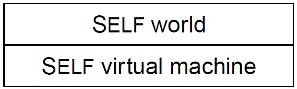
\includegraphics{Chapter_1_Figure_1.png}}
\caption{Figure 1: The Self system}\end{flushleft}\end{figure}

The VM executes Self programs specified by objects in the Self world and provides a set of \emph{primitives} (which are methods written in C++) that can be invoked by Self methods to carry out basic operations like integer arithmetic, object copying, and I/O. The Self world distributed with the VM is a collection of Self objects implementing various \emph{traits} and \emph{prototypes} like cloning traits and dictionaries. These objects can be used (or changed) to implement your own programs.
\begin{figure}[htbp]\begin{flushleft}
\capstart

\scalebox{1.000000}{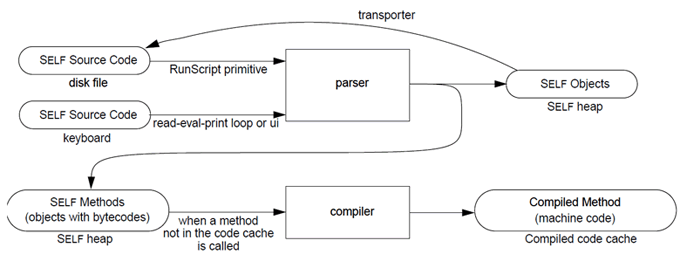
\includegraphics{Chapter_1_Figure_2.png}}
\caption{Figure 2: How Self programs are compiled.}\end{flushleft}\end{figure}

\index{bytecodes}
\index{compilation}
\index{customization}
Self programs are translated to machine code in a two-stage process (see Figure 2). Code typed in at the prompt, through the user interface, or read in from a file is parsed into Self objects. Some of these objects are data objects; others are methods. Methods have their own behavior which they represent with \emph{bytecodes}. The bytecodes are the instructions for a very simple virtual processor that understands instructions like “push receiver” or “send the ‘x’ message.” In fact, Self bytecodes correspond much more closely to source code than, say, Smalltalk-80 bytecodes. (See {\hyperref[ref:citations]{\emph{{[}CUL89{]}}}} for a list of the Self byte codes.) The \emph{raison d’être} of the virtual machine is to pretend that these bytecodes are directly executed by the computer; the programmer can explore the Self world down to the bytecode level, but no further. This pretense ensures that the behavior of a Self program can be understood by looking only at the Self source code.

The second stage of translation is the actual \emph{compilation} of the bytecodes to machine code. This is how the “execution” of bytecodes is implemented—it is totally invisible on the Self level except for side effects like execution speed and memory usage. The compilation takes place the first time a message is actually sent; thus, the first execution of a program will be slower than subsequent executions.

Actually, this explanation is not entirely accurate: the compiled method is specialized on the type of the receiver. If the same message is later sent to a receiver of different type (e.g., a float instead of an integer), a new compilation takes place. This technique is called \emph{customization}; see {\hyperref[ref:citations]{\emph{{[}CU89{]}}}} for details. Also, the compiled methods are placed into a cache from which they can be flushed for various reasons; therefore, they might be recompiled from time to time. Furthermore, the current version of the compiler will recompile and reoptimize frequently used code, using information gathered at run-time as to how the code is being used; see {\hyperref[ref:citations]{\emph{{[}HCU91{]}}}} for details.

Don’t be misled by the term “compiled method” if you are familiar with Smalltalk: in Smalltalk terminology it denotes a method in its bytecode form, but in Self it denotes the native machine code form. In Smalltalk there is only one compiled method per source method, but in Self there may be several different compiled methods for the same source method (because of customization).


\chapter{Language Reference}
\label{langref:language-reference}\label{langref::doc}
This chapter specifies Self’s syntax and semantics. An early version of the syntax was presented
in the original Self paper by Ungar and Smith {\hyperref[ref:citations]{\emph{{[}US87{]}}}} ; this chapter incorporates subsequent
changes to the language. The presentation assumes a basic understanding of object-oriented concepts.

The syntax is described using Extended Backus-Naur Form (EBNF). Terminal symbols appear in
Courier and are enclosed in single quotes; they should appear in code as written (not including
the single quotes). Non-terminal symbols are italicized. The following table describes the metasymbols:

\begin{tabulary}{\linewidth}{|L|L|L|}
\hline

META-SYMBOL
 & 
FUNCTION
 & 
DESCRIPTION
\\\hline

( and )
 & 
grouping
 & 
used to group syntactic constructions
\\\hline

{[} and {]}
 & 
option
 & 
encloses an optional construction
\\\hline

\{ and \}
 & 
repetition
 & 
encloses a construction that may be repeated zero or more times
\\\hline

\textbar{}
 & 
alternative
 & 
separates alternative constructions
\\\hline

\(\rightarrow\)
 & 
production
 & 
separates the left and right hand sides of a production
\\\hline
\end{tabulary}


A glossary of terms used in this document can be found in Appendix A.

\index{block}
\index{object}
\index{slot}

\section{Objects}
\label{langref:objects}\label{langref:index-2}
\emph{Objects} are the fundamental entities in Self; every entity in a Self program is represented by one
or more objects. Even control is handled by objects: \emph{blocks} (\S{}2.1.7) are Self closures used to implement
user-defined control structures. An object is composed of a (possibly empty) set of \emph{slots}
and, optionally, \emph{code} (\S{}2.1.5). A slot is a name-value pair; slots contain references to other objects.
When a slot is found during a \emph{message lookup} (\S{}2.3.6) the object in the slot is evaluated.

Although everything is an object in Self, not all objects serve the same purpose; certain kinds of
objects occur frequently enough in specialized roles to merit distinct terminology and syntax. This
chapter introduces two kinds of objects, namely data objects (“plain” objects) and the two kinds of
objects with code, ordinary methods and block methods.

\index{object literals}

\subsection{Syntax}
\label{langref:syntax}\label{langref:index-3}
\emph{Object literals} are delimited by parentheses. Within the parentheses, an object description consists
of a list of slots delimited by vertical bars (‘\textbar{}’), followed by the code to be executed when the object
is evaluated. For example:
\begin{quote}

\begin{Verbatim}[commandchars=\\\{\}]
( \textbar{} slot1. slot2 \textbar{} ’here is some code’ printLine )
\end{Verbatim}
\end{quote}

Both the slot list and code are optional: ‘( \textbar{} \textbar{} )’ and ‘()’ each denote an empty object. \footnote{
If you wish to use the empty vertical bar notation to create an empty object, note that the parser currently requires a space between the vertical bars.
}

\emph{Block objects} are written like other objects, except that square brackets (‘{[}’ and ‘{]}’) are used in
place of parentheses:
\begin{quote}

\begin{Verbatim}[commandchars=\\\{\}]
[ \textbar{} slot1. slot2 \textbar{} ’here is some code in a block’ printLine ]
\end{Verbatim}
\end{quote}

A \emph{slot list} consists of a (possibly empty) sequence of \emph{slot descriptors} (\S{}2.2) separated by periods.
A period at the end of the slot list is optional. \footnote{
But in that case make sure you put a space after the period, otherwise you will get an obscure error message from the parser.
}

The code for an object is a sequence of \emph{expressions} (\S{}2.3) separated by periods. A trailing period
is optional. Each expression consists of a series of \emph{message sends} and \emph{literals}. The last expression
in the code for an object may be preceded by the ‘\textasciicircum{}’ operator (\S{}2.1.8).

\index{object!data object}
\index{empty object}

\subsection{Data objects}
\label{langref:index-5}\label{langref:data-objects}
\emph{Data objects} are objects without code. Data objects can have any number of slots. For example, the
object () has no slots (i.e., it’s empty) while the object ( \textbar{} x = 17. y = 18 \textbar{} ) has two slots,
x and y.
\begin{figure}[htbp]\begin{flushleft}

\scalebox{1.000000}{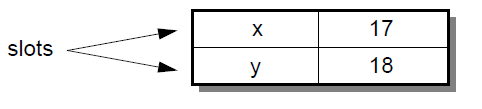
\includegraphics{Chapter_2_Image_1.png}}
\end{flushleft}\end{figure}

A data object returns itself when evaluated.

\index{assignment primitive}
\index{code}
\index{non-local return operator}
\index{assignment slot}
\index{slot list}

\subsection{The assignment primitive}
\label{langref:the-assignment-primitive}\label{langref:index-10}
A slot containing the assignment primitive is called an \emph{assignment slot} (\S{}2.2.2). When an assignment
slot is evaluated, the argument to the message is stored in the corresponding \emph{data slot} (\S{}2.2)
in the same object (the slot whose name is the assignment slot’s name minus the trailing colon),
and the \emph{receiver} (\S{}2.3) is returned as the result. (Note: this means that the value of an assignment
statement is the left-hand side of the assignment statement, not the right-hand side as it is in Smalltalk,
C, and many other languages. This is a potential source of confusion for new Self programmers.)

\index{self slot}
\index{argument slot}
\index{self}
\index{object!method object}
\index{method activation object}
\index{method}
\index{evaluation!of arguments}
\index{evaluation!of message sends}

\subsection{Objects with code}
\label{langref:objects-with-code}\label{langref:index-18}
The feature that distinguishes a \emph{method object} from a data object is that it has \emph{code}, whereas a data
object does not. Evaluating a method object does not simply return the object itself, as with simple
data objects; rather, its code is executed and the resulting value is returned.


\subsection{Code}
\label{langref:code}
\emph{Code} is a sequence of \emph{expressions} (\S{}2.3). These expressions are evaluated in order, and the resulting
values are discarded except for that of the final expression, whose value determines the result
of evaluating the code.

The actual arguments in a message send are evaluated from left to right before the message is sent.
For instance, in the expression:
\begin{quote}

\begin{Verbatim}[commandchars=\\\{\}]
1 to: 5 \PYGZbs{}* i By: 2 \PYGZbs{}* j Do: [\PYGZbs{}\textbar{}:k \PYGZbs{}\textbar{} k print ]
\end{Verbatim}
\end{quote}

1 is evaluated first, then 5 * i, then 2 * j, and then {[}\textbar{}:k \textbar{} k print{]}. Finally, the to:By:Do:
message is sent. The associativity and precedence of messages is discussed in section 4.

\index{activation object}

\subsection{Methods}
\label{langref:methods}\label{langref:index-19}
\emph{Ordinary methods} (or simply “methods”) are methods that are not embedded in other code. A
method can have \emph{argument slots} (\S{}2.2.3) and/or local slots. An ordinary method always has an implicit
\emph{parent} (\S{}2.2.4) argument slot named self. Ordinary methods are Self’s equivalent of
Smalltalk’s methods.

If a slot contains a method, the following steps are performed when the slot is evaluated as the result
of a message send:
\begin{itemize}
\item {} 
The method object is \emph{cloned}, creating a new \emph{method activation object} containing slots for the method’s arguments and locals.

\item {} 
The clone’s self parent slot is initialized to the receiver of the message.

\item {} 
The clone’s argument slots, if any, are initialized to the values of the corresponding actual arguments.

\item {} 
The code of the method is executed in the context of this new activation object.

\end{itemize}

For example, consider the method ( \textbar{} :arg \textbar{} arg * arg ):
\begin{figure}[htbp]\begin{flushleft}

\scalebox{1.000000}{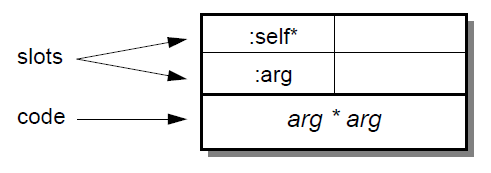
\includegraphics{Chapter_2_Image_2.png}}
\end{flushleft}\end{figure}

This method has an argument slot arg and returns the square of its argument.

\index{slot!anonymous parent slot}
\index{block}
\index{block!block data object}
\index{traits object}
\index{anonymous parent}
\index{non-lifo block}
\index{evaluation!of blocks}

\subsection{Blocks}
\label{langref:blocks}\label{langref:index-26}
\emph{Blocks} are Self closures; they are used to implement user-defined control structures. A block literal
(delimited by square brackets) defines two objects: the \emph{block method object}, containing the
block’s code, and an enclosing \emph{block data object}. The block data object contains a parent pointer
(pointing to the object containing the shared behavior for block objects) and a slot containing the
block method object. Unlike an ordinary method object, the block method object does not contain
a self slot. Instead, it has an anonymous parent slot that is initialized to point to the activation object
for the lexically enclosing block or method. As a result, \emph{implicit-receiver messages} (\S{}2.3.4)
sent within a block method are lexically scoped. The block method object’s anonymous parent slot
is invisible at the Self level and cannot be accessed explicitly.

For example, the block {[} 3 + 4 {]} looks like: \footnote{
All block objects have the same parent, an object containing the shared behavior for blocks
}
\begin{figure}[htbp]\begin{flushleft}

\scalebox{1.000000}{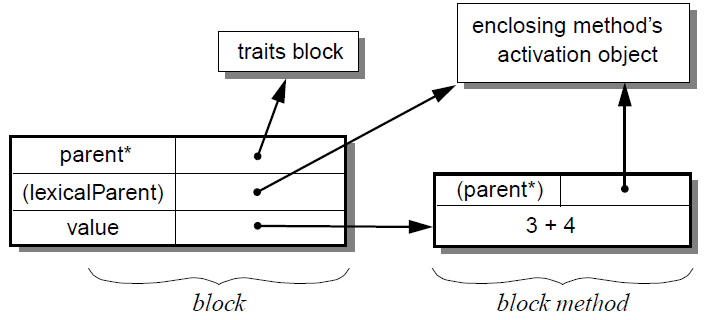
\includegraphics{Chapter_2_Image_3.png}}
\end{flushleft}\end{figure}

The block method’s selector is based on the number of arguments. If the block takes no arguments,
the selector is \code{value}. If it takes one argument, the selector is \code{value:}. If it takes two arguments,
the selector is \code{value:With:}, for three the selector is \code{value:With:With:}, and for more the selector
is just extended by enough \code{With:’s} to match the number of block arguments.

Block evaluation has two phases. In the first phase, a block object is created because the block is
evaluated (e.g., it is used as an argument to a message send). The block is cloned and given a
pointer to the activation record for its lexically enclosing scope, the current activation record. In the
second phase, the block’s method is evaluated as a result of sending the block the appropriate variant
of the \code{value} message. The block method is then cloned, the argument slots of the clone are
filled in, the anonymous parent slot of the clone is initialized using the scope pointer determined in
phase one, and, finally, the block’s code is executed.

It is an error to evaluate a block method after the activation record for its lexically enclosing scope
has returned. Such a block is called a \emph{non-lifo} block because returning from it would violate the
last-in, first-out semantics of activation object invocation.

This restriction is made primarily to allow activation records to be allocated from a stack. A future
release of Self may relax this restriction, at least for blocks that do not access variables in
enclosing scopes.

\index{non-local return}

\subsection{Returns}
\label{langref:returns}\label{langref:index-27}
A \emph{return} is denoted by preceding an expression by the ‘\textasciicircum{}’ operator. A return causes the value of the given expression to be returned as the result of evaluating the method or block. Only the last ex­pression in an object may be a return.

The presence or absence of the ‘\textasciicircum{}’ operator does not effect the behavior of ordinary methods, since an ordinary method always returns the value of its final expression anyway. In a block, however, a return causes control to be returned from the ordinary method containing that block, immediately terminating that method’s activation, the block’s activation, and all activations in between. Such a return is called a \emph{non-local return}, since it may “return through” a number of activations. The result of the ordinary method’s evaluation is the value returned by the \emph{non-local return}. For example, in the following method:
\begin{quote}

\begin{Verbatim}[commandchars=\\\{\}]
assertPositive: x = (
                x \textgreater{} 0 ifTrue: [ \textasciicircum{} ’ok’ ].
                error: ’non-positive x’ )
\end{Verbatim}
\end{quote}

the \code{error:} message will not be sent if x is positive because the non-local return of ‘ok’ causes the \code{assertPositive:} method to return immediately.

\index{object literals!construction of}

\subsection{Construction of object literals}
\label{langref:index-28}\label{langref:construction-of-object-literals}
Object literals are constructed during parsing—the parser converts objects in textual form into real Self objects.
An object literal is constructed as follows:
\begin{itemize}
\item {} 
First, the slot initializers of every slot are evaluated from left to right. If a slot initializer contains
another object literal, this literal is constructed before the initializer containing it is evaluated.
If the initializer is an expression, it is evaluated in the context of the lobby.

\item {} 
Second, the object is created, and its slots are initialized with the results of the evaluations performed
in the first step.

\end{itemize}

Slot initializers are \emph{not} evaluated in the lexical context, since none exists at parse time; they are evaluated
in the context of an object known as the \code{lobby}. That is, the initializers are evaluated as if they were the code
of a method in a slot of the \code{lobby}. This two-phase object construction pro­cess implies that slot initializers may
not refer to any other slots within the constructed object (as with Scheme’s \code{let*} and \code{letrec} forms) and, more generally,
that a slot initializer may not refer to any textually enclosing object literal.

\index{root context}
\index{assignment slot}
\index{data slot}
\index{slot!read/write slot}
\index{slot!read-only slot}

\section{Slot descriptors}
\label{langref:slot-descriptors}\label{langref:index-33}
An object can have any number of slots. Slots can contain data (\emph{data slots}) or methods. Some slots have special roles: \emph{argument slots} are filled in with the actual arguments during a message send (\S{}2.3.3), and \emph{parent slots} specify inheritance relationships (\S{}2.3.8).

A \emph{slot descriptor} consists of an optional privacy specification, followed by the slot name and an optional initializer.


\subsection{Read-only slots}
\label{langref:read-only-slots}
A slot name followed by an equals sign (‘=’) and an expression represents a \emph{read-only slot} initialized to the result of evaluating the expression in the root context.

For example, a constant point might be defined as:
\begin{quote}

\begin{Verbatim}[commandchars=\\\{\}]
( \textbar{}     parent* = traits point.
        x = 3 + 4.
        y = 5.
\textbar{} )
\end{Verbatim}
\end{quote}

The resulting point contains three initialized read-only slots:
\begin{figure}[htbp]\begin{flushleft}

\scalebox{1.000000}{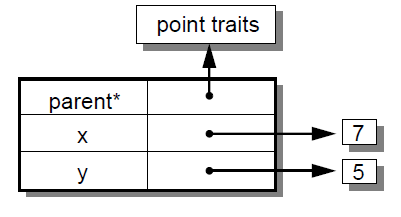
\includegraphics{Chapter_2_Image_4.png}}
\end{flushleft}\end{figure}

\index{self slot!self slot}
\index{slot!assignable data slot}
\index{self}
\index{read/write variable}

\subsection{Read/write slots}
\label{langref:read-write-slots}\label{langref:index-37}
There is no separate assignment operation in Self. Instead, assignments to data slots are message sends that invoke the assignment primitive. For example, a data slot x is assignable if and only if there is a slot in the same object with the same name appended with a colon (in this case, x:), containing the assignment primitive. Therefore, assigning 17 to slot x consists of sending the message x: 17. Since this is indistinguishable from a message send that invokes a method, clients do not need to know if x and x: comprise data slot accesses or method invocations.

An identifier followed by a left arrow (the characters ‘\textless{}’ and ‘-’ concatenated to form ‘\textless{}-’) and an expression represents an initialized \emph{read/write variable} (assignable data slot). The object will contain both a data slot of that name and a corresponding assignment slot whose name is obtained by appending a colon to the data slot name. The initializing expression is evaluated in the root context and the result stored into the data slot at parse time.

For example, an initialized mutable point might be defined as:
\begin{quote}

\begin{Verbatim}[commandchars=\\\{\}]
( \textbar{}     parent* = traits point.
        x \textless{}- 3 + 4.
        y \textless{}- 5.
\textbar{} )
\end{Verbatim}
\end{quote}

producing an object with two data slots (xand y) and two assignment slots (x:and y:) containing the assignment primitive (depicted with ←): \footnote{
In the user interface a read/write slot is depicted as a single slot with a colon labelling the button used to access the value of the slot; the assignment slot is not shown, to save screen space. In contrast, a read-only slot has an equals sign on the button.
}
\begin{figure}[htbp]\begin{flushleft}

\scalebox{1.000000}{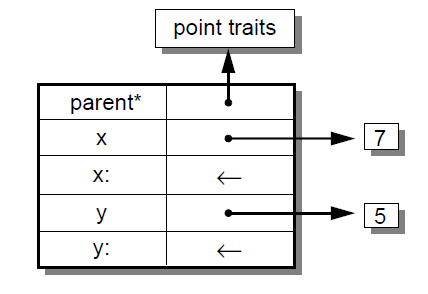
\includegraphics{Chapter_2_Image_5.png}}
\end{flushleft}\end{figure}

An identifier by itself specifies an assignable data slot initialized to \emph{nil} . \footnote{
Nil is a predefined object provided by the implementation. It is intended to indicate “not a useful object.”
} Thus, the slot declaration x is a shorthand notation for x \textless{}- nil.

For example, a simple mutable point might be defined as:
\begin{quote}

\begin{Verbatim}[commandchars=\\\{\}]
( \textbar{} x. y. \textbar{} )
\end{Verbatim}
\end{quote}

producing:
\begin{figure}[htbp]\begin{flushleft}

\scalebox{1.000000}{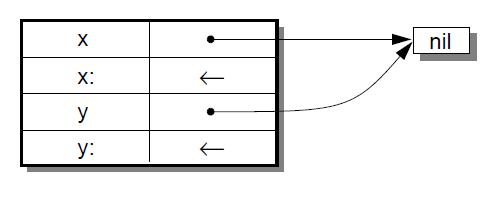
\includegraphics{Chapter_2_Image_6.png}}
\end{flushleft}\end{figure}

\index{slot!argument slot}
\index{message!keyword message}

\subsection{Slots containing methods}
\label{langref:index-39}\label{langref:slots-containing-methods}
If the initializing expression is an object literal with code, that object is stored into the slot \emph{without evaluating the code}. This allows a slot to be initialized to a method by storing the method itself, rather than its result, in the slot. \footnote{
Although a block may be assigned to a slot at any time, it is often not useful to do so: evaluating the slot may result in an error because the activation record for the block’s lexically enclosing scope will have returned; see \S{}2.1.7.
} Methods may only be stored in read-only slots. A method automatically receives a parent argument slot named self. For example, a point addition method can be written as:
\begin{quote}

\begin{Verbatim}[commandchars=\\\{\}]
( \textbar{}
                + = ( \textbar{} :arg \textbar{} (clone x: x + arg x) y: y + arg y ).
\textbar{} )
\end{Verbatim}
\end{quote}

producing:
\begin{figure}[htbp]\begin{flushleft}

\scalebox{1.000000}{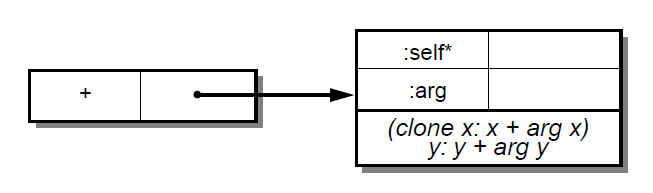
\includegraphics{Chapter_2_Image_7.png}}
\end{flushleft}\end{figure}

A slot name beginning with a colon indicates an \emph{argument} slot. The prefixed colon is not part of the slot name and is ignored when matching the name against a message. Argument slots are always read-only, and no initializer may be specified for them. As a syntactic convenience, the argument name may also be written immediately after the slot name (without the prefixed colon), thereby implicitly declaring the argument slot. Thus, the following yields exactly the same object as above:
\begin{quote}

\begin{Verbatim}[commandchars=\\\{\}]
( \textbar{}
        + arg = ( (clone x: x + arg x) y: y + arg y ).
\textbar{} )
\end{Verbatim}
\end{quote}

The + slot above is a \emph{binary slot} (\S{}2.3.2), taking one argument and having a name that consists of operator symbols. Slots like x or y in a point object are \emph{unary slots} (\S{}2.3.1), which take no arguments and have simple identifiers for names. In addition, there are \emph{keyword slots} (\S{}2.3.3), which handle messages that require one or more arguments. A keyword slot name is a sequence of identifiers, each followed by a colon.

The arguments in keyword methods are handled analogously to those in binary methods: each colon-terminated identifier in a keyword slot name requires a corresponding argument slot in the keyword method object, and the argument slots may be specified either all in the method or all interspersed with the selector parts.

For example:
\begin{quote}

\begin{Verbatim}[commandchars=\\\{\}]
( \textbar{}
        ifTrue: False: = ( \textbar{} :trueBlock. :falseBlock \textbar{}
                trueBlock value ).
\textbar{} )
\end{Verbatim}
\end{quote}

and
\begin{quote}

\begin{Verbatim}[commandchars=\\\{\}]
( \textbar{}
        ifTrue: trueBlock False: falseBlock =
                ( trueBlock value ).
\textbar{} )
\end{Verbatim}
\end{quote}

produce identical objects.

\index{slot!parent slot}

\subsection{Parent slots}
\label{langref:parent-slots}\label{langref:index-40}
A unary slot name followed by an asterisk denotes a \emph{parent slot}. The trailing asterisk is not part of the slot name and is ignored when matching the name against a message. Except for their special meaning during the message lookup process (\S{}2.3.8), parent slots are exactly like normal unary slots; in particular, they may be assignable, allowing \emph{dynamic inheritance}. Argument slots cannot be parent slots.

\index{annotation separator}
\index{Annotations}

\subsection{Annotations}
\label{langref:annotations}\label{langref:index-42}
In order to provide extra information for the programming environment, Self supports annotations on either whole objects or individual slots. Although any object can be an annotation, the Self syntax only supports the textual definition of string annotations. In order to annotate an object, use this syntax:
\begin{quote}

\begin{Verbatim}[commandchars=\\\{\}]
( \textbar{} \PYGZob{}\PYGZcb{} = ’this object has one slot’ snort = 17. \textbar{} ) \PYGZcb{}
\end{Verbatim}
\end{quote}

In order to annotate a group of slots, surround them with braces and insert the annotation after the opening brace:
\begin{quote}

\begin{Verbatim}[commandchars=\\\{\}]
( \textbar{}
        \PYGZob{} ’Category: accessing’
                getOne = (...).
                getAnother = (...).
        \PYGZcb{}
        anUnannotatedSlot.
\textbar{} )
\end{Verbatim}
\end{quote}

Annotations may nest; if so the Virtual Machine concatenates the annotations strings and inserts a separator character (16r7f). \footnote{
The current programming environment expects a slot annotation to start with one of a number of keywords, including ``Category: '', ``Comment: '', and ``ModuleInfo:''. See the programming environment manual for more details.
}


\section{Expressions}
\label{langref:expressions}
\emph{Expressions} in Self are \emph{messages} sent to some object, the \emph{receiver}. Self message syntax is similar to Smalltalk’s. Self provides three basic kinds of messages: unary messages, binary messages, and keyword messages. Each has its own syntax, associativity, and precedence. Each type of message can be sent either to an explicit or implicit receiver.

Productions: \footnote{
In order to simplify the presentation, this grammar is ambiguous; precedence and associativity rules are used to resolve the ambiguities.
}

\begin{tabulary}{\linewidth}{|L|L|L|}
\hline

expression
 & 
\(\rightarrow\)
 & 
constant \textbar{} unary-message \textbar{} binary-message \textbar{} keyword-message \textbar{} ‘(’ expression ‘)’
\\\hline

constant
 & 
\(\rightarrow\)
 & 
self \textbar{} number \textbar{} string \textbar{} object
\\\hline

unary-message
 & 
\(\rightarrow\)
 & 
receiver unary-send \textbar{} resend ‘.’ unary-send
\\\hline

unary-send
 & 
\(\rightarrow\)
 & 
identifier
\\\hline

binary-message
 & 
\(\rightarrow\)
 & 
receiver binary-send \textbar{} resend ‘.’ binary-send
\\\hline

binary-send
 & 
\(\rightarrow\)
 & 
operator expression
\\\hline

keyword-message
 & 
\(\rightarrow\)
 & 
receiver keyword-send \textbar{} resend ‘.’ keyword-send
\\\hline

keyword-send
 & 
\(\rightarrow\)
 & 
small-keyword expression \{ cap-keyword expression \}
\\\hline

receiver
 & 
\(\rightarrow\)
 & 
{[} expression {]}
\\\hline

resend
 & 
\(\rightarrow\)
 & 
resend \textbar{} identifier
\\\hline
\end{tabulary}


The table below summarizes Self’s message syntax rules:

\begin{tabulary}{\linewidth}{|L|L|L|L|L|}
\hline

MESSAGE
 & 
ARGUMENTS
 & 
PRECEDENCE
 & 
ASSOCIATIVITY
 & 
SYNTAX
\\\hline

Unary
 & 
0
 & 
highest
 & 
none
 & 
{[}receiver{]} identifier
\\\hline

binary
 & 
1
 & 
medium
 & 
none or left-to-right*
 & 
{[}receiver{]} operator expression
\\\hline

keyword
 & 
≥ 1
 & 
lowest
 & 
right-to-left
 & 
{[}receiver{]} small-keyword expression \{ cap-keyword expression \}
\\\hline
\end{tabulary}


* Heterogeneous binary messages have no associativity; homogeneous binary messages associate left-to-right.

Parentheses can be used to explicitly specify order of evaluation.

\index{associativity!of unary messages}
\index{message!unary message}

\subsection{Unary messages}
\label{langref:unary-messages}\label{langref:index-44}
A \emph{unary message} does not specify any arguments. It is written as an identifier following the receiver.

Examples of unary messages sent to explicit receivers:
\begin{quote}

\begin{Verbatim}[commandchars=\\\{\}]
17 print
5 factorial
\end{Verbatim}
\end{quote}

\emph{Associativity}. Unary messages compose from left to right. An expression to print 5 factorial, for example, is written:
\begin{quote}

\begin{Verbatim}[commandchars=\\\{\}]
5 factorial print
\end{Verbatim}
\end{quote}

and interpreted as:
\begin{quote}

\begin{Verbatim}[commandchars=\\\{\}]
(5 factorial) print
\end{Verbatim}
\end{quote}

\emph{Precedence}. Unary messages have higher precedence than binary messages and keyword messages.

\index{associativity!of binary messages}
\index{message!binary message}
\index{precedence of message sends}

\subsection{Binary messages}
\label{langref:index-47}\label{langref:binary-messages}
A \emph{binary message} has a receiver and a single argument, separated by a binary operator. Examples of binary messages:
\begin{quote}

\begin{Verbatim}[commandchars=\\\{\}]
3 + 4
7 \textless{}-\textgreater{} 8
\end{Verbatim}
\end{quote}

\emph{Associativity}. Binary messages have no associativity, except between identical operators (which associate from left to right). For example,
\begin{quote}

\begin{Verbatim}[commandchars=\\\{\}]
\PYG{l+m+mi}{3} \PYG{o}{+} \PYG{l+m+mi}{4} \PYG{o}{+} \PYG{l+m+mi}{7}
\end{Verbatim}
\end{quote}

is interpreted as
\begin{quote}

\begin{Verbatim}[commandchars=\\\{\}]
\PYG{p}{(}\PYG{l+m+mi}{3} \PYG{o}{+} \PYG{l+m+mi}{4}\PYG{p}{)} \PYG{o}{+} \PYG{l+m+mi}{7}
\end{Verbatim}
\end{quote}

But
\begin{quote}

\begin{Verbatim}[commandchars=\\\{\}]
\PYG{l+m+mi}{3} \PYG{o}{+} \PYG{l+m+mi}{4} \PYG{o}{*} \PYG{l+m+mi}{7}
\end{Verbatim}
\end{quote}

is illegal: the associativity must be made explicit by writing either
\begin{quote}

\begin{Verbatim}[commandchars=\\\{\}]
(3 + 4) * 7 or 3 + (4 * 7).
\end{Verbatim}
\end{quote}

\emph{Precedence}. The precedence of binary messages is lower than unary messages but higher than keyword messages. All binary messages have the same precedence. For example,
\begin{quote}

\begin{Verbatim}[commandchars=\\\{\}]
3 factorial + pi sine
\end{Verbatim}
\end{quote}

is interpreted as
\begin{quote}

\begin{Verbatim}[commandchars=\\\{\}]
(3 factorial) + (pi sine)
\end{Verbatim}
\end{quote}

\index{associativity!of keyword messages}
\index{keyword message}
\index{primitive send}

\subsection{Keyword messages}
\label{langref:index-50}\label{langref:keyword-messages}
A \emph{keyword message} has a receiver and one or more arguments. It is written as a receiver followed by a sequence of one or more keyword-argument pairs. The first keyword must begin with a lower case letter or underscore (‘\_’); subsequent keywords must be capitalized. An initial underscore denotes that the operation is a \emph{primitive}. A keyword message consists of the longest possible sequence of such keyword-argument pairs; the message selector is the concatenation of the keywords forming the message. Message selectors beginning with an underscore are reserved for \emph{primitives} (\S{}2.3.7).

Example:
\begin{quote}

\begin{Verbatim}[commandchars=\\\{\}]
5 min: 4 Max: 7
\end{Verbatim}
\end{quote}

is the single message min:Max: sent to 5 with arguments 4 and 7, whereas
\begin{quote}

\begin{Verbatim}[commandchars=\\\{\}]
5 min: 4 max: 7
\end{Verbatim}
\end{quote}

involves two messages: first the message max:sent to 4 and taking 7 as its argument, and then the message min: sent to 5, taking the result of (4 max: 7) as its argument.

\emph{Associativity}. Keyword messages associate from right to left, so
\begin{quote}

\begin{Verbatim}[commandchars=\\\{\}]
5 min: 6 min: 7 Max: 8 Max: 9 min: 10 Max: 11
\end{Verbatim}
\end{quote}

is interpreted as
\begin{quote}

\begin{Verbatim}[commandchars=\\\{\}]
5 min: (6 min: 7 Max: 8 Max: (9 min: 10 Max: 11))
\end{Verbatim}
\end{quote}

The association order and capitalization requirements are intended to reduce the number of parentheses necessary in Self code. For example, taking the minimum of two slots mand nand storing the result into a data slot i may be written as
\begin{quote}

\begin{Verbatim}[commandchars=\\\{\}]
i: m min: n
\end{Verbatim}
\end{quote}

Precedence. Keyword messages have the lowest precedence. For example,
\begin{quote}

\begin{Verbatim}[commandchars=\\\{\}]
i: 5 factorial + pi sine
\end{Verbatim}
\end{quote}

is interpreted as
\begin{quote}

\begin{Verbatim}[commandchars=\\\{\}]
i: ((5 factorial) + (pi sine))
\end{Verbatim}
\end{quote}

\index{message!implicit-receiver message}

\subsection{Implicit-receiver messages}
\label{langref:implicit-receiver-messages}\label{langref:index-51}
Unary, binary, and keyword messages are frequently written without an explicit receiver. Such messages use the current receiver (\code{self}) as the implied receiver. The method lookup, however, begins at the current activation object rather than the current receiver (see \S{}2.1.4 for details on activation objects). Thus, a message sent explicitly to \code{self} is \emph{not} equivalent to an implicit-receiver send because the former won’t search local slots before searching the receiver. Explicitly sending messages to \code{self} is considered bad style.

Examples:
\begin{quote}

\begin{Verbatim}[commandchars=\\\{\}]
factorial               (implicit-receiver unary message)
+ 3                     (implicit-receiver binary message)
max: 5                  (implicit-receiver keyword message)
1 + power: 3            (parsed as 1 + (power: 3))
\end{Verbatim}
\end{quote}

Accesses to slots of the receiver (local or inherited) are also achieved by implicit message sends to \code{self}. For an assignable data slot named \code{t}, the message \code{t} returns the contents, and \code{t}: 17 puts 17 into the slot.

\index{resend}
\index{directed resend}

\subsection{Resending messages}
\label{langref:index-53}\label{langref:resending-messages}
A \emph{resend} allows an overridding method to invoke the overridden method. Directed resends allow ambiguities among overridden methods to be resolved by constraining the lookup to search a single parent slot. Both resends and directed resends may change the name of the message being sent from the name of the current method, and may pass different arguments than the arguments passed to the current method. The receiver of a resend or a directed resend must be the implicit receiver.

Intuitively, resend is similar to Smalltalk’s \code{supersend} and CLOS’ \code{call-next-method}.

A resend is written as an implicit-receiver message with the reserved word \code{resend}, a period, and the message name. No whitespace may separate \code{resend}, the period, and the message name.

Examples:
\begin{quote}

\begin{Verbatim}[commandchars=\\\{\}]
resend.display
resend.+ 5
resend.min: 17 Max: 23
\end{Verbatim}
\end{quote}

A \emph{directed resend} constrains the resend through a specified parent. It is written similar to a normal resend, but replaces \code{resend} with the name of the parent slot through which the resend is directed.

Examples:
\begin{quote}

\begin{Verbatim}[commandchars=\\\{\}]
listParent.height
intParent.min: 17 Max: 23
\end{Verbatim}
\end{quote}

Only implicit-receiver messages may be delegated via a resend or a directed resend. \footnote{
General delegation for explicit receiver messages is supported through primitives in the implementation (see Appendix 9.8).
}

\index{message semantics}

\subsection{Message lookup semantics}
\label{langref:message-lookup-semantics}\label{langref:index-54}
This section describes the semantics of message lookups in Self. In addition to an informal textual description, the lookup semantics are presented in pseudo-code using the following notation:
\begin{quote}

\begin{tabulary}{\linewidth}{|L|L|}
\hline

s.name
 & 
The name of slot s.
\\\hline

s.contents
 & 
The object contained in slot s.
\\\hline

s.isParent
 & 
True iff s is a parent slot.
\\\hline

\{s \(\epsilon\) obj \textbar{} pred(s)\}
 & 
The set of all slots of object obj that satisfy predicate pred.
\\\hline

\textbar{} S \textbar{}
 & 
The cardinality of set S.
\\\hline
\end{tabulary}

\end{quote}

The message sending semantics are decomposed into the following functions:
\begin{quote}

\begin{tabulary}{\linewidth}{|L|L|}
\hline

send(rec, sel, args)
 & 
The message send function (\S{}2.3.7).
\\\hline

lookup(obj, rec, sel, V)
 & 
The lookup algorithm (\S{}2.3.8).
\\\hline

undirected\_resend(...)
 & 
The undirected message resend function (\S{}2.3.9).
\\\hline

directed\_resend(...)
 & 
The directed message resend function (\S{}2.3.9).
\\\hline

\emph{eval(rec, M, args)}
 & 
The slot evaluation function as described informally throughout \S{}2.1.
\\\hline
\end{tabulary}

\end{quote}


\subsection{Message send}
\label{langref:message-send}
There are two kinds of message sends: a \emph{primitive send} has a selector beginning with an underscore (‘\_’) and calls the corresponding primitive operation. Primitives are predefined functions provided by the implementation. A \emph{normal send} does a lookup to obtain the target slot; if the lookup was successful, the slot is subsequently evaluated. If the slot contains a data object, then the data object is simply returned. If the slot contains the assignment primitive, the argument of the message is stored in the corresponding data slot. Finally, if the slot contains a method, an activation is created and run as described in \S{}2.1.6.

If the lookup fails, the lookup error is handled in an implementation-defined manner; typically, a message indicating the type of error is sent to the object which could not handle the message.

The function \emph{send(rec, sel, args)} is defined as follows:
\begin{quote}
\begin{description}
\item[{\textbf{Input}:}] \leavevmode
\begin{DUlineblock}{0em}
\item[] rec, the receiver of the message
\item[] sel, the message selector
\item[] args, the actual arguments
\end{DUlineblock}

\item[{\textbf{Output}:}] \leavevmode
\begin{DUlineblock}{0em}
\item[] res, the result object
\end{DUlineblock}

\end{description}

\textbf{Algorithm}
\begin{quote}

\begin{Verbatim}[commandchars=\\\{\}]
if begins\_with\_underscore(sel)
then invoke\_primitive(rec, sel, args)                   “primitive call”
else M ← lookup(rec, sel, Ø)                            “do the lookup”
        case
                \textbar{} M \textbar{} = 0: error: message not understood
                \textbar{} M \textbar{} = 1: res ← eval(rec, M, args)     “see \S{}2.1”
                \textbar{} M \textbar{} \textgreater{} 1: error: ambiguous message send
        end
end
return res
\end{Verbatim}
\end{quote}
\end{quote}

\index{lookup algorithm}

\subsection{The lookup algorithm}
\label{langref:the-lookup-algorithm}\label{langref:index-55}
The lookup algorithm recursively traverses the inheritance graph, which can be an arbitrary graph (including cyclic graphs). No object is searched twice along any single path. The search begins in the object itself and then continues to search every parent. Parent slots are not evaluated during the lookup. That is, if a parent slot contains an object with code, the code will not be executed; the object will merely be searched for matching slots.

The function \emph{lookup(obj, sel, V)} is defined as follows:
\begin{quote}
\begin{description}
\item[{\textbf{Input}:}] \leavevmode
\begin{DUlineblock}{0em}
\item[] obj, the object being searched for matching slots
\item[] sel, the message selector
\item[] V, the set of objects already visited along this path
\end{DUlineblock}

\item[{\textbf{Output}:}] \leavevmode
\begin{DUlineblock}{0em}
\item[] M, the set of matching slots
\end{DUlineblock}

\end{description}

\textbf{Algorithm}:
\begin{quote}

\begin{Verbatim}[commandchars=\\\{\}]
if obj \(\epsilon\) V
then M ← Ø                                                      “cycle detection”
else M ← \PYGZob{}s \(\epsilon\) obj \textbar{} s.name = sel\PYGZcb{}                               “try local slots”
        if M = Ø then M ← parent\_lookup(obj, sel, V) end        “try    parent slots”
end
return M
\end{Verbatim}
\end{quote}
\end{quote}

Where \emph{parent\_lookup(obj, sel, V)} is defined as follows:
\begin{quote}

\begin{Verbatim}[commandchars=\\\{\}]
P ← \PYGZob{}s \(\epsilon\) obj \textbar{} s.isParent\PYGZcb{}                                      “all parents”
M ← \(\upsilon\) lookup(s.contents, sel, V \(\upsilon\) \PYGZob{}obj\PYGZcb{})                        “recursively search parents”
   s\(\epsilon\)P
return M
\end{Verbatim}
\end{quote}


\subsection{Undirected Resend}
\label{langref:undirected-resend}
An undirected resend ignores the sending method holder (the object containing the currently running method) and continues with its parents.

The function \emph{undirected\_resend(rec, smh, sel, args)} is defined as follows:
\begin{quote}
\begin{description}
\item[{\textbf{Input}:}] \leavevmode
\begin{DUlineblock}{0em}
\item[] rec, the receiver of the message
\item[] smh, the sending method holder
\item[] sel, the message selector args, the actual arguments
\end{DUlineblock}

\item[{\textbf{Output}:}] \leavevmode
\begin{DUlineblock}{0em}
\item[] res, the result object
\end{DUlineblock}

\end{description}

\textbf{Algorithm}:
\begin{quote}

\begin{Verbatim}[commandchars=\\\{\}]
M ← parent\_lookup(smh, sel, Ø)                                  “do the lookup”
case
        \textbar{} M \textbar{} = 0: error: message not understood
        \textbar{} M \textbar{} = 1: res ← eval(rec, M, args)                     “see \S{}2.1”
        \textbar{} M \textbar{} \textgreater{} 1: error: ambiguous message send
end
return res
\end{Verbatim}
\end{quote}
\end{quote}


\subsection{Directed Resend}
\label{langref:directed-resend}
A directed resend looks only in one slot in the sending method holder.

The function \emph{directed\_resend(rec, smh, del, sel, args)} is defined as follows:
\begin{quote}
\begin{description}
\item[{\textbf{Input}:}] \leavevmode
\begin{DUlineblock}{0em}
\item[] rec, the receiver of the message
\item[] smh, the sending method holder
\item[] del, the name of the delegatee
\item[] sel, the message selector
\item[] args, the actual arguments
\end{DUlineblock}

\item[{\textbf{Output}:}] \leavevmode
\begin{DUlineblock}{0em}
\item[] res, the result object
\end{DUlineblock}

\end{description}

\textbf{Algorithm}:
\begin{quote}

\begin{Verbatim}[commandchars=\\\{\}]
D ← \PYGZob{}s \(\epsilon\) smh \textbar{} s.name = del\PYGZcb{}                            “find delegatee”
if \textbar{} D \textbar{} = 0 then error: missing delegatee              “one or none”
M ← lookup(smh.del, sel, Ø)                             “do the lookup”
case
        \textbar{} M \textbar{} = 0: error: message not understood
        \textbar{} M \textbar{} = 1: res ← eval(rec, M, args)             “see \S{}2.1”
        \textbar{} M \textbar{} \textgreater{} 1: error: ambiguous message send
end
return res
\end{Verbatim}
\end{quote}
\end{quote}


\section{Lexical elements}
\label{langref:lexical-elements}
This chapter describes the lexical structure of Self programs—how sequences of characters in Self source code are grouped into lexical tokens. In contrast to syntactic elements described by productions in the rest of this document, the elements of lexical EBNF productions may not be separated by whitespace, i.e. there may not be whitespace within a lexical token. Tokens are formed from the longest sequence of characters possible. Whitespace may separate any two tokens and must separate tokens that would be treated as one token otherwise.

\index{character set}

\subsection{Character set}
\label{langref:index-56}\label{langref:character-set}
Self programs are written using the following characters:
\begin{itemize}
\item {} 
\emph{Letters}. The fifty-two upper and lower case letters: ABCDEFGHIJKLMNOPQRSTUVWXYZabcdefghijklmnopqrstuvwxyz

\item {} 
\emph{Digits}. The ten numeric digits: 0123456789

\item {} 
\emph{Whitespace}. The formatting characters: space, horizontal tab (ASCII HT), newline (NL), carriage return (CR), vertical tab (VT), backspace (BS), and form feed (FF). (Comments are also treated as whitespace.)

\item {} 
\emph{Graphic characters}. The 32 non-alphanumeric characters: !@\#\$\%\textasciicircum{}\&*()\_-+=\textbar{}\textbackslash{}\textasciitilde{}‘\{\}{[}{]}:;''’\textless{}\textgreater{},.?/

\end{itemize}

\index{self}
\index{resend}
\index{identifier}
\index{primitive}

\subsection{Identifiers}
\label{langref:identifiers}\label{langref:index-60}
An \emph{identifier} is a sequence of letters, digits, and underscores (‘\_’) beginning with a lowercase letter or an underscore. Case is significant: \code{apoint} is not the same as \code{aPoint}.

Productions:
\begin{quote}

\begin{tabulary}{\linewidth}{|L|L|L|}
\hline

small-letter
 & 
\(\rightarrow\)
 & 
‘a’ \textbar{} ‘b’ \textbar{} ... \textbar{} ‘z’
\\\hline

cap-letter
 & 
\(\rightarrow\)
 & 
‘A’ \textbar{} ‘B’ \textbar{} ... \textbar{} ‘Z’
\\\hline

letter
 & 
\(\rightarrow\)
 & 
small-letter \textbar{} cap-letter
\\\hline

identifier
 & 
\(\rightarrow\)
 & 
(small-letter \textbar{} ‘\_’) \{letter \textbar{} digit \textbar{} ‘\_’\}
\\\hline
\end{tabulary}

\end{quote}

Examples: \code{i \_IntAdd cloud9 m a\_point}

The two identifiers \code{self} and \code{resend} are reserved. Identifiers beginning with underscores are reserved for primitives.

\index{Keywords}

\subsection{Keywords}
\label{langref:keywords}\label{langref:index-61}
Keywords are used as slot names and as message names. They consist of an identifier or a capitalized identifier followed by a colon (‘:’).

Productions:
\begin{quote}

\begin{tabulary}{\linewidth}{|L|L|L|}
\hline

small-keyword
 & 
\(\rightarrow\)
 & 
identifier ‘:’
\\\hline

cap-keyword
 & 
\(\rightarrow\)
 & 
cap-letter \{letter \textbar{} digit \textbar{} ‘\_’\} ‘:’
\\\hline
\end{tabulary}

\end{quote}

Examples: \code{at:} \code{Put:} \code{\_IntAdd:}

\index{argument slot}

\subsection{Arguments}
\label{langref:index-62}\label{langref:arguments}
A colon followed by an identifier denotes an \emph{argument} slot name.

Productions:
\begin{quote}

\begin{tabulary}{\linewidth}{|L|L|L|}
\hline

arg-name
 & 
\(\rightarrow\)
 & 
‘:’ identifier
\\\hline
\end{tabulary}

\end{quote}

Example: \code{:name}

\index{operator}

\subsection{Operators}
\label{langref:operators}\label{langref:index-63}
An \emph{operator} consists of a sequence of one or more of the following characters:

! @ \# \$ \% \textasciicircum{} \& * - + = \textasciitilde{} / ? \textless{} \textgreater{} , ; \textbar{} ‘ \textbackslash{}

Two sequences are reserved and are not operators:

\textbar{} \textasciicircum{}

Productions:
\begin{quote}

\begin{tabulary}{\linewidth}{|L|L|L|}
\hline

op-char
 & 
\(\rightarrow\)
 & 
‘!’ \textbar{} ‘@’ \textbar{} ‘\#’ \textbar{} ‘\$’ \textbar{} ‘\%’ \textbar{} ‘\textasciicircum{}’ \textbar{} ‘\&’ \textbar{} ‘*’ \textbar{} ‘-’ \textbar{} ‘+’ \textbar{} ‘=’ \textbar{} ‘\textasciitilde{}’ \textbar{} ‘/’ \textbar{} ‘?’ \textbar{}‘\textless{}’ \textbar{} ‘\textgreater{}’ \textbar{} ‘,’ \textbar{} ‘;’ \textbar{} ‘\textbar{}’ \textbar{} ‘‘’ \textbar{} ‘’
\\\hline

operator
 & 
\(\rightarrow\)
 & 
op-char \{op-char\}
\\\hline
\end{tabulary}

\end{quote}

Examples: + - \&\& \textbar{}\textbar{} \textless{}-\textgreater{} \% \# @ \textasciicircum{}

\index{Numbers}
\index{non-decimal number}

\subsection{Numbers}
\label{langref:index-65}\label{langref:numbers}
Integer literals are written as a sequence of digits, optionally prefixed with a minus sign and/or a
base. \footnote{
Unlike Smalltalk, integer literals are limited in range to smallInts.
} No whitespace is allowed between a minus sign and the digit sequence. \footnote{
In situations where parsing the minus sign as part of the number would cause a parse error (for example, in the expression a-1), the minus is interpreted as a binary message (a - 1).
} Real constants may
be either written in fixed-point or exponential form.

Integers may be written using bases from 2 to 36. For bases greater than ten, the characters ‘\emph{a}’
through ‘\emph{z}’ (case insensitive) represent digit values 10 through 35. The default base is decimal. A
non-decimal number is prefixed by its base value, specified as a decimal number followed by either
‘\emph{r}’ or ‘\emph{R}’.

Real numbers may be written in decimal only. The exponent of a floating-point format number indicates
multiplication of the mantissa by 10 raised to the exponent power; i.e.,

nnnnEddd = nnnn × 10 $^{\text{ddd}}$

A number with a digit that is not appropriate for the base will cause a lexical error, as will an integer
constant that is too large to be represented. If the absolute value of a real constant is too large
or too small to be represented, the value of the constant will be \(\pm\) infinity or zero, respectively.

Productions:
\begin{quote}

\begin{tabulary}{\linewidth}{|L|L|L|}
\hline

number
 & 
\(\rightarrow\)
 & 
{[} ‘-’ {]} (integer \textbar{} real)
\\\hline

integer
 & 
\(\rightarrow\)
 & 
{[}base{]} general-digit \{general-digit\}
\\\hline

real
 & 
\(\rightarrow\)
 & 
fixed-point \textbar{} float
\\\hline

fixed-point
 & 
\(\rightarrow\)
 & 
decimal ‘.’ decimal
\\\hline

float
 & 
\(\rightarrow\)
 & 
decimal {[} ‘.’ decimal {]} (‘e’ \textbar{} ‘E’) {[} ‘+’ \textbar{} ‘-’ {]} decimal
\\\hline

general-digit
 & 
\(\rightarrow\)
 & 
digit \textbar{} letter
\\\hline

decimal
 & 
\(\rightarrow\)
 & 
digit \{digit\}
\\\hline

base
 & 
\(\rightarrow\)
 & 
decimal (‘r’ \textbar{} ‘R’)
\\\hline
\end{tabulary}

\end{quote}

Examples: 123 16r27fe 1272.34e+15 1e10

\index{character escapes}
\index{String constants}
\index{string escape sequences}

\subsection{Strings}
\label{langref:strings}\label{langref:index-68}
String constants are enclosed in single quotes (‘’’). With the exception of single quotes and escape
sequences introduced by a backslash (‘\textbackslash{}’), all characters (including formatting characters like
newline and carriage return) lying between the delimiting single quotes are included in the string. \footnote{
When typing strings in, the graphical user interface accepts multi-line strings, but the character-based read-evalprint loop does not.
}

To allow single quotes to appear in a string and to allow non-printing control characters in a string
to be indicated more visibly, Self provides C-like escape sequences:
\begin{quote}

\begin{tabulary}{\linewidth}{|L|L|L|L|L|L|}
\hline

\textbackslash{}t
 & 
tab
 & 
\textbackslash{}b
 & 
backspace
 & 
\textbackslash{}n
 & 
newline
\\\hline

\textbackslash{}f
 & 
form feed
 & 
\textbackslash{}r
 & 
carriage return
 & 
\textbackslash{}v
 & 
vertical tab
\\\hline

\textbackslash{}a
 & 
alert (bell)
 & 
\textbackslash{}0
 & 
null character
 & 
\textbackslash{} \textbackslash{}
 & 
backslash
\\\hline

\textbackslash{}’
 & 
single quote
 & 
\textbackslash{}''
 & 
double quote
 & 
\textbackslash{}?
 & 
question mark
\\\hline
\end{tabulary}

\end{quote}

A backslash followed by an ‘x’, ‘d’, or ‘o’ specifies the character with the corresponding numeric
encoding in the ASCII character set:
\begin{quote}

\begin{tabulary}{\linewidth}{|L|L|}
\hline

\textbackslash{}xnn
 & 
hexadecimal escape
\\\hline

\textbackslash{}dnnn
 & 
decimal escape
\\\hline

\textbackslash{}onnn
 & 
octal escape
\\\hline
\end{tabulary}

\end{quote}

There must be exactly two hexadecimal digits for hexadecimal character escapes, and exactly three
digits for decimal and octal character escapes. Illegal hexadecimal, decimal, and octal numbers, as
well as character escapes specifying ASCII values greater than 255 will cause a lexical error.

For example, the following characters all denote the carriage return character (ASCII code 13):
\begin{quote}

\begin{tabulary}{\linewidth}{|L|L|L|L|}
\hline

\textbackslash{}r
 & 
\textbackslash{}x0d
 & 
\textbackslash{}d013
 & 
\textbackslash{}o015
\\\hline
\end{tabulary}

\end{quote}

A long string may be broken into multiple lines by preceding each newline with a backslash. Such
escaped newlines are ignored during formation of the string constant.

A backslash followed by any other character than those listed above will cause a lexical error.

Productions:
\begin{quote}

\begin{tabulary}{\linewidth}{|L|L|L|}
\hline

string
 & 
\(\rightarrow\)
 & 
‘’’ \{ normal-char \textbar{} escape-char \} ‘’’
\\\hline

normal-char
 & 
\(\rightarrow\)
 & 
any character except ‘\textbackslash{}’ and ‘’’
\\\hline

escape-char
 & 
\(\rightarrow\)
 & 
‘\textbackslash{}t’ \textbar{} ‘\textbackslash{}b’ \textbar{} ‘\textbackslash{}n’ \textbar{} ‘\textbackslash{}f’ \textbar{} ‘\textbackslash{}r’ \textbar{} ‘\textbackslash{}v’ \textbar{} ‘\textbackslash{}a’ \textbar{} ‘\textbackslash{}0’ \textbar{} ‘\textbackslash{} \textbackslash{}’ \textbar{} ‘\textbackslash{}’’ \textbar{} ‘\textbackslash{}''’ \textbar{} ‘\textbackslash{}?’ \textbar{} numeric-escape
\\\hline

numeric-escape
 & 
\(\rightarrow\)
 & 
‘\textbackslash{}x’ general-digit general-digit \textbar{} ( ‘\textbackslash{}d’ \textbar{} ‘\textbackslash{}o’ ) digit digit digit
\\\hline
\end{tabulary}

\end{quote}


\subsection{Comments}
\label{langref:comments}
Comments are delimited by double quotes (‘''’). Double quotes may not themselves be embedded
in the body of a comment. All characters (including formatting characters like newline and carriage
return) are part of the body of a comment.

Productions:
\begin{quote}

\begin{tabulary}{\linewidth}{|L|L|L|}
\hline

comment
 & 
\(\rightarrow\)
 & 
‘''’ \{ comment-char \} ‘''’
\\\hline

comment-char
 & 
\(\rightarrow\)
 & 
any character except ‘''’
\\\hline
\end{tabulary}

\end{quote}

Example: ``this is a comment''

\index{block}
\index{block!block method}
\index{block!non-lifo block}
\index{block!non-local return}
\index{cloning}
\index{closure}
\index{message}
\index{binary message}
\index{implicit-receiver message}
\index{keyword message}
\index{unary message}
\index{method!outer method}
\index{method holder}
\index{method holder!sending method holder}
\index{non-local return}
\index{object}
\index{data object}
\index{primitive send}
\index{selector}
\index{sending method holder}
\index{slot}
\index{data slot}
\index{comments}
\index{traits object}
\index{parent slot}
\index{argument slot}
\index{root context}
\index{resend}
\index{prototype}
\index{parent slot}
\index{nil}
\index{message!message lookup}
\index{lookup}
\index{inheritance}
\index{inheritance!dynamic inheritance}

\chapter{The Self World}
\label{selfwrld::doc}\label{selfwrld:the-self-world}
The default Self world is a set of useful objects, including objects that can be used in application
programs (e.g., integers, strings, and collections), objects that support the programming environment
(e.g., the debugger), and objects that simply are used to organize the other objects. This document
describes how this world is organized, focusing primarily on those objects meant for use in
Self programs. It does not discuss the objects used to implement system facilities—for example,
there is no discussion of the objects used to implement the graphical user interface—nor does it
discuss how to use programming support objects such as the command history object; such tools
are described in The Self User’s Manual.

The reader is assumed to be acquainted with the Self language, the use of multiple inheritance,
the use of traits objects and prototype objects, and the organizing principles of the Self world as
discussed in {\hyperref[ref:citations]{\emph{{[}UCC91{]}}}}.


\section{World Organization}
\label{worldorg::doc}\label{worldorg:world-organization}

\subsection{The Lobby}
\label{worldorg:the-lobby}
The lobby object is thus named because it is where objects enter the Self world. For example,
when a script that creates a new object is read into the system, all expressions in that script are evaluated
in the context of the lobby. That is, the lobby is the receiver of all messages sent to “self” by
expressions in the script. To refer to some existing object in a script, the object must be accessible
by sending a message to the lobby. For example, the expression:

\begin{Verbatim}[commandchars=\\\{\}]
\_AddSlots: ( \textbar{} newObject = ( \textbar{} entries \textless{}- list copy ... \textbar{} ) \textbar{} )
\end{Verbatim}

requires that the message \code{list} be understood by the lobby (the implicit receiver of the message)
so that the \code{entries} slot of the new object can be initialized. The lobby slots \code{traits}, \code{globals},
and \code{mixins} are the roots of the object namespaces accessible from the lobby. The organization of
these namespaces is described in the next section. The slot \code{lobby} allows the lobby itself to be referred
by name.

The lobby also has a number of other functions: it is the location of the default behavior inherited
by most objects in the system (slot \code{defaultBehavior}).


\subsection{Names and Paths}
\label{worldorg:names-and-paths}
For convenience, the lobby’s namespace is broken into three pieces, implemented as separate objects
rooted at the lobby:
\begin{quote}
\begin{description}
\item[{traits}] \leavevmode
objects that encapsulate shared behavior. Typically, each prototype object has an associated traits object of the same name that describes the shared part of its behavior.

\item[{globals}] \leavevmode
prototypical objects and one-of-a-kind objects (“oddballs”)

\item[{mixins}] \leavevmode
small, parentless bundles of behavior designed to be “mixed into” some other object

\end{description}
\end{quote}

Each of these namespace objects is categorized to aid navigation.

For example, to find the parent of the prototype list object, one could start with the \code{globals} slot
of the lobby, then get the \code{list} slot of that object, and then the \code{parent} slot of the list. The sequence
of slot names, \code{globals list parent} is called a \emph{path} and constitutes the list parent’s
\emph{full name}. Parent slots can be omitted from an object’s full name, since the slots in a parent are visible
in the child via inheritance. A path with parent slots omitted forms the \emph{short name} for an object.
For example, the short name for the list parent is simply \code{list parent}.

Non-parent slots are used when it is desirable to keep a part of the name space distinct. For example,
the \code{traits} slot of the lobby is not a parent slot. This allows a convention that gives prototypes
and their associated traits objects similar names: a prototype and its associated traits object have
the same local name, but the prototype is placed in a slot in the \code{globals} object, whereas the traits
of the prototype is placed in a slot in the \code{traits} object. Since the \code{traits} slot of the lobby is not
a parent slot, the name of the traits object must start with the prefix \code{traits}. The \code{globals} slot,
on the other hand, is a parent slot, so the name of a prototype object needs no prefix. Thus, \code{list}
refers to the prototype list while \code{traits list} refers to its traits object for lists.

As a matter of style, programs should refer to objects by the shortest possible name. This makes it
easier to re-organize the global namespace as the system evolves. (If programs used full path
names, then many more names would have to be updated to reflect changes to the namespace organization,
a tedious chore.)


\section{The Roots of Behavior}
\label{roots::doc}\label{roots:the-roots-of-behavior}

\subsection{Default Behavior}
\label{roots:default-behavior}
Certain common behavior is shared by nearly all objects in the Self world. This basic behavior is
defined in the \code{defaultBehavior} slot of the lobby and includes:
\begin{itemize}
\item {} 
identity comparisons (== and !==)

\item {} 
inequality (!=)

\item {} 
default behavior for printing (reimplement printString in descendants)

\item {} 
mirror creation (reflect:)

\item {} 
support for point, and list construction (@ and \&)

\item {} 
behavior that allows blocks to ignore extra arguments

\item {} 
behavior that allows an object to behave like a block that evaluates to that object (this permits a non-block object to be passed to a method that expects a block)

\item {} 
behavior that allows an object to be its own key in a collection (key)

\item {} 
default behavior for doubly-dispatched messages

\item {} 
behavior for printing error messages and stack dumps (error: and halt)

\end{itemize}

It is important to note that not all objects in the system inherit this default behavior. It is entirely
permissible to construct objects that do not inherit from the lobby, and the Self world contains
quite a few such objects. For example, the objects used to break a namespace into separate categories
typically do not inherit from the lobby. Any program intended to operate on arbitrary objects,
such as a debugger, must therefore assume that the objects it manipulates do not understand even
the messages in \code{defaultBehavior}.

Modules: defaultBehavior, errorHandling


\subsection{The Root Traits: Traits Clonable and Traits Oddball}
\label{roots:the-root-traits-traits-clonable-and-traits-oddball}
Most concrete objects in the Self world are descendants of one of two top-level traits objects:
\code{traits clonable} and \code{traits oddball}. The distinction between the two is based on whether
or not the object is \emph{unique}. For example, \code{true} is a unique object. There is only one \code{true} object in
the entire system, although there are many references to it. On the other hand, a list object is not
unique. There may be many lists in the system, each containing different elements. A unique object
responds to the message \code{copy} by returning itself and uses identity to test for equality. The general
rule is:
\begin{itemize}
\item {} 
unique objects usually inherit from \code{traits oddball}

\item {} 
non-unique objects usually inherit from \code{traits clonable}

\end{itemize}

Module: rootTraits


\subsection{Mixins}
\label{roots:mixins}
Like traits objects, mixin objects encapsulate a bundle of shared behavior. Unlike traits objects,
however, mixin objects are generally parentless to allow their behavior to be added to an object
without necessarily also adding unwanted behavior (such as access to the lobby namespace). Mixins
are generally used in objects that also have other parents. An example is \code{mixins identity}.


\subsection{The Identity Mixin}
\label{roots:the-identity-mixin}
Two objects are usually tested for equality based on whether they have “the same value” within a
common domain. For example, \code{3.0 = 3} within the domain of numbers, even though they are not
the same object or even the same kind of object. In some domains, however, two objects are equal
if and only if they are the exact same object. For example, even two process objects with the same
state are not considered equal unless they are identical. In such cases, identity comparison is used
to implement equality tests, and \code{mixins identity} can be mixed in to get the desired behavior.

Module: rootTraits


\section{Blocks, Booleans, and Control Structures}
\label{blocks:blocks-booleans-and-control-structures}\label{blocks::doc}
A \emph{block} is a special kind of object containing a sequence of statements. When a block is evaluated
by being sent an acceptable \code{value} message, its statements are executed in the context of the current
activation of the method in which the block is declared. This allows the statements in the block
to access variables local to the block’s enclosing method and any enclosing blocks in that method.
(This set of variables comprises the lexical scope of the block.) It also means that within the block,
\code{self} refers to the receiver of the message that activated the method, not to the block object itself.
A return statement in a block causes a return from the block’s enclosing method. (See the Self
Language Reference for a more thorough discussion of block semantics.)
A block can take an arbitrary number of arguments and can have its own local variables, as well as
having access to the local variables of its enclosing method. The statements in the block are executed
when the block is sent a message of the form \code{“value{[}:\{With:\}{]}”}, where the number of colons
in the message is at least the same as the number of arguments the block takes (extra
arguments are ignored, but it is an error to provide too few). For example, the following block takes
two arguments:

\begin{Verbatim}[commandchars=\\\{\}]
[\textbar{} :arg1. :arg2 \textbar{} arg1 + arg2 ]
\end{Verbatim}

and can be evaluated by sending it the message \code{value:With:} to produce the sum of its arguments.
Blocks are used to implement all control structures in Self and allow the programmer to
easily extend the system with customized control structures. In fact, all control stuctures in Self
except message sends, returns, and VM error handling are implemented using blocks.


\subsection{Booleans and Conditionals}
\label{blocks:booleans-and-conditionals}
The fundamental control structure is the conditional. In Self, the behavior of conditionals is defined
by two unique boolean objects, \code{true} and \code{false}. Boolean objects respond to the messages
\code{ifTrue:}, \code{ifFalse:}, \code{ifTrue:False:}, and \code{ifFalse:True:} by evaluating the appropriate argument
block. For example, \code{true} implements \code{ifTrue:False:} as:

\begin{Verbatim}[commandchars=\\\{\}]
ifTrue: b1 False: b2 = ( b1 value )
\end{Verbatim}

That is, when \code{true} is sent \code{ifTrue:False:}, it evaluates the first block and ignores the second.
For example, the following expression evaluates to the absolute value of x:

\begin{Verbatim}[commandchars=\\\{\}]
x \textless{} 0 ifTrue: [ x negate ] False: [ x ]
\end{Verbatim}

The booleans also define behavior for the logical operations \code{AND (\&\&), OR (\textbar{}\textbar{}), EXCLUSIVE-OR
(\textasciicircum{}\textasciicircum{})}, and \code{NOT (not)}. Because the binary boolean operators all send value to their argument when
necessary, they can also be used for “short-circuit” evaluation by supplying a block, e.g.:

\begin{Verbatim}[commandchars=\\\{\}]
(0 \textless{}= i) \&\& [i \textless{} maxByte pred] ifTrue: [...
\end{Verbatim}

Module: boolean


\subsection{Loops}
\label{blocks:loops}
The various idioms for constructing loops in Self are best illustrated by example.
Here is an endless loop:

\begin{Verbatim}[commandchars=\\\{\}]
[ ... ] loop
\end{Verbatim}

Here are two loops that test for their termination condition at the beginning of the loop:

\begin{Verbatim}[commandchars=\\\{\}]
[ proceed ] whileTrue: [ ... ]
[ quit ] whileFalse: [ ... ]
\end{Verbatim}

In each case, the block that receives the message repeatedly evaluates itself and, if the termination
condition is not yet met, evaluates the argument block. The value returned by both loop expressions
is \code{nil}.

It is also possible to put the termination test at the end of the loop, ensuring that the loop body is
executed at least once:

\begin{Verbatim}[commandchars=\\\{\}]
[ ... ] untilTrue: [ quit ]
[ ... ] untilFalse: [ proceed ]
\end{Verbatim}

Here is a loop that exits from the middle when quit becomes true:

\begin{Verbatim}[commandchars=\\\{\}]
[\textbar{} :exit \textbar{} ... quit ifTrue: exit ... ] loopExit
\end{Verbatim}

For the incurably curious: the parameter to the user’s block, supplied by the \code{loopExit} method, is simply a block that
does a return from the \code{loopExit} method. Thus, the loop terminates when \code{exit value} is evaluated. The constructs
\code{loopExitValue}, \code{exit}, and \code{exitValue} are implemented in a similar manner.

The value returned by the overall “{[}...{]} loopExit” expression is nil. Here is a loop expression
that exits and evaluates to a value determined by the programmer when quit becomes true:

\begin{Verbatim}[commandchars=\\\{\}]
[\textbar{} :exit \textbar{} ... quit ifTrue: [ exit value: expr ] ] loopExitValue
\end{Verbatim}

Module: block


\subsection{Block Exits}
\label{blocks:block-exits}
It is sometimes convenient to exit a block early, without executing its remaining statements. The
following constructs support this behavior:

\begin{Verbatim}[commandchars=\\\{\}]
[\textbar{} :exit \textbar{} ... quit ifTrue: exit ... ] exit
[\textbar{} :exit \textbar{} ... quit ifTrue: [ exit value: expr ] ... ] exitValue
\end{Verbatim}

The first expression evaluates to nil if the block exits early; the second allows the programmer to
define the expression’s value when the block exits early. Note: These constructs should not be confused
with their looping counterparts \code{loopExit} and \code{loopExitValue}.

Module: block


\subsection{Other Block Behavior}
\label{blocks:other-block-behavior}
Blocks have some other useful behavior:
\begin{itemize}
\item {} 
One can determine the time in milliseconds required to execute a block using various ways of measuring time using the messages \code{userTime}, \code{systemTime}, \code{cpuTime}, and \code{real-Time}.

\item {} 
One can profile the execution of a block using the messages \code{profile} and \code{flatProfile}. \code{profile} prints out the source level call graph annotated with call site and timing information       whereas \code{flatProfile} prints out a flat profile sorted by module.

\item {} 
The message \code{countSends} will collect lookup statistics during a block execution.

\end{itemize}

Any object that inherits from the lobby can be passed to a method that expects a block; behavior in{}`{}`defaultBehavior{}`{}` makes the object behave like a block that evaluates to that object.

Module: block


\section{Numbers and Time}
\label{numbers:numbers-and-time}\label{numbers::doc}
The SELF number traits form the hierarchy shown below. (In this and subsequent hierarchy descriptions,
indentation indicates that one traits object is a child of another. The prefix “traits” is
omitted since these hierarchy descriptions always describe the interrelationship between traits objects.
In most cases, leaf traits are concrete and have an associated prototype with the same name.)
\begin{quote}

\begin{Verbatim}[commandchars=\\\{\}]
orderedOddball
        number
                float
                integer
                        smallInt
                        bigInt
\end{Verbatim}
\end{quote}

\code{traits number} defines behavior common to all numbers, such as \code{successor}, \code{succ}, \code{predecessor},
\code{pred}, \code{absoluteValue}, \code{negate}, \code{double}, \code{half}, \code{max:}, and \code{min:}. \code{traits number}
inherits from \code{traits orderedOddball}, so sending \code{copy} or \code{clone} to a number returns the
number itself. \code{traits integer} defines behavior common to all integers such as \code{even}, \code{odd}, and
\code{factorial}. There are four division operators for integers that allow the programmer to control
how the result is truncated or rounded. Integers also include behavior for iterating through a subrange,
including:

\begin{Verbatim}[commandchars=\\\{\}]
to:Do:
to:By:Do:
to:ByNegative:Do:
upTo:Do:
upTo:By:Do:
downTo:Do:
downTo:By:Do:
\end{Verbatim}

Relevant oddballs:
\begin{itemize}
\item {} 
infinity IEEE floating-point infinity

\item {} 
minSmallInt smallest smallInt in this implementation

\item {} 
maxSmallInt biggest smallInt in this implementation

\end{itemize}

Modules: number, float, integer, smallInt, bigInt


\subsection{Random Numbers}
\label{numbers:random-numbers}\begin{quote}

\begin{Verbatim}[commandchars=\\\{\}]
clonable
random
randomLC
prototypes random
\end{Verbatim}
\end{quote}

\code{Traits random} defines the abstract behavior of random number generators. A random number
generator can be used to generate random booleans, integers, floats, characters or strings. \code{traits
randomLC} defines a concrete specialization based on a simple linear congruence algorithm. For
convenience, the prototype for \code{randomLC} is “\code{random},” not “\code{randomLC}”.

Modules: random


\subsection{Time}
\label{numbers:time}\begin{quote}

\begin{Verbatim}[commandchars=\\\{\}]
\PYG{n}{clonable}
\PYG{n}{time}
\end{Verbatim}
\end{quote}

A time object represents a date and time (to the nearest millisecond) since midnight GMT on January
1, 1970. The message \code{current} returns a new time object containing the current time. Two
times can be compared using the standard comparison operators. One time can be subtracted from
another to produce a value in milliseconds. An offset in milliseconds can be added or subtracted
from a time object to produce a new time object. However, it is an error to add two time objects
together.

Modules: time


\section{Collections}
\label{collections:collections}\label{collections::doc}\begin{quote}

\begin{Verbatim}[commandchars=\\\{\}]
clonable
        collection
                ... collection hierarchy ...
\end{Verbatim}
\end{quote}

Collections are containers that hold zero or more other objects. In Self, collections behave as if
they have a key associated with each value in the collection. Collections without an obvious key,
such as lists, use each element as both key and value. Iterations over collections always pass both
the value and the key of each element (in that order) to the iteration block. Since Self blocks ignore
extra arguments, this allows applications that don’t care about keys to simply provide a block
that takes only one argument.

Collections have a rich protocol. Additions are made with \code{at:Put:}, or with \code{add:} or \code{addAll:} for
implicitly keyed collections. Iteration can be done with do: or with variations that allow the programmer
to specify special handling of the first and/or last element. \code{with:Do:} allows pairwise iteration
through two collections. The \code{includes:}, \code{occurrencesOf:}, and \code{findFirst:}
\code{IfPresent:IfAbsent:} messages test for the presence of particular values in the collection.
\code{filterBy:Into:} creates a new collection including only those elements that satisfy a predicate
block, while \code{mapBy:Into:} creates a new collection whose elements are the result of applying the
argument block to each element of the original collection.

Abstract collection behavior is defined in traits collection. Only a small handful of operations need
be implemented to create a new type of collection; the rest can be inherited from \code{traits collection}.
(See the \code{descendantResponsibility} slot of \code{traits collection}.) The following
sections discuss various kinds of collection in more detail.

Modules: collection (abstract collection behavior)


\subsection{Indexable Collections}
\label{collections:indexable-collections}\begin{quote}

\begin{Verbatim}[commandchars=\\\{\}]
collection
        indexable
                mutableIndexable
                        byteVector
                                ...the string hierarchy
                        sequence
                                sortedSequence
                        vector
\end{Verbatim}
\end{quote}

Indexable collections allow random access to their elements via keys that are integers. All sequences
and vectors are indexable. The message \code{at:} is used to retrieve an element of an indexable collection
while \code{at:Put:} is used to update an element of a \code{mutableIndexable} collection (other
than a \code{sortedSequence}).

Modules: indexable, abstractString, vector, sequence, sortedSequence


\subsection{Strings, Characters, and Paragraphs}
\label{collections:strings-characters-and-paragraphs}\begin{quote}

\begin{Verbatim}[commandchars=\\\{\}]
collection
        ...
        byteVector
                string
                        mutableString
                        immutableString
                                canonicalString
\end{Verbatim}
\end{quote}

A string is a vector whose elements are character objects. There are three kinds of concrete string:
immutable strings, mutable strings and canonical strings. \code{traits string} defines the behavior
shared by all strings. A character is a string of length one that references itself in its sole indexable
slot.

Mutable strings can be changed using the message \code{at:Put:}, which takes a character argument, or
\code{at:PutByte:}, which takes an integer argument. An immutable string cannot be modified, but
sending it the \code{copyMutable} message returns a mutable string containing the same characters.

Canonical strings are registered in an table inside the virtual machine, like Symbol objects in
Smalltalk or atoms in LISP. The VM guarantees that there is at most one canonical string for any
given sequence of bytes, so two canonical strings are equal (have the same contents) if and only if
they are identical (are the same object). This allows efficient equality checks between canonical
strings. All message selectors and string literals are canonical strings, and some primitives require
canonical strings as arguments. Sending \code{canonicalize} to any string returns the corresponding
canonical string.

Character objects behave like immutable strings of length one. There are 256 well-known character
objects in the Self universe. They are stored in a 256-element vector named \code{ascii}, with each
character stored at the location corresponding to its ASCII value. Characters respond to the message
\code{asByte} by returning their ASCII value (that is, their index in \code{ascii}). The inverse of \code{asByte},
\code{asCharacter}, can be sent to an integer between 0 and 255 to obtain the corresponding
character object.

Module: string


\subsection{Unordered Sets and Dictionaries}
\label{collections:unordered-sets-and-dictionaries}\begin{quote}

\begin{Verbatim}[commandchars=\\\{\}]
collection
        setOrDictionary
                set
                        sharedSet
                dictionary
                        sharedDictionary
\end{Verbatim}
\end{quote}

There are two implementations of sets and dictionaries in the system. The one described in this
section is based on hash tables. The one discussed in the following section is based on sorted binary
trees. The hash table implementation has better performance over a wide range of conditions.
(An unfortunate ordering of element addtions can cause the unbalanced trees used in the tree version
to degenerate into an ordered lists, resulting in linear access times.)

A set behaves like a mathematical set. It contains elements without duplication in no particular order.
A dictionary implements a mapping from keys to values, where both keys and values are arbitrary
objects. Dictionaries implement the usual collection behavior plus keyed access using \code{at:}
and \code{at:Put:} and the dictionary-specific operations \code{includesKey:} and \code{removeKey:}. In order
to store an object in a set or use it as a dictionary key, the object must understand the messages
\code{hash} and \code{=}, the latter applying to any pair of items in the collection. This is because sets and dictionaries
are implemented as hash tables.

Derived from set and dictionary are \code{sharedSet} and \code{sharedDictionary}. These provide locking
to maintain internal consistency in the presence of concurrency.

Modules: setAndDictionary, sharedSetAndDictionary


\subsection{Tree-Based Sets and Dictionaries}
\label{collections:tree-based-sets-and-dictionaries}\begin{quote}

\begin{Verbatim}[commandchars=\\\{\}]
collection
        tree
                treeNodes abstract
                        treeNodes bag
                        treeNodes set
                emptyTrees abstract
                        emptyTrees bag
                        emptyTrees set
\end{Verbatim}
\end{quote}

\code{treeSet} and \code{treeBag} implement sorted collections using binary trees. The set variant ignores
duplicates, while the bag variant does not. Tree sets and bags allow both explicit and implicit keys
(that is, adding elements can be done with either \code{at:Put:} or \code{add:}), where a tree set that uses
explicit keys behaves like a dictionary. Sorting is done on explicit keys if present, values otherwise,
and the objects sorted must be mutually comparable. Comparisons between keys are made using
\code{compare:IfLess:Equal:Greater:}.

The implementation of trees uses dynamic inheritance to distinguish the differing behavior of empty
and non-empty subtrees. The prototype \code{treeSet} represents an empty (sub)tree; when an element
is added to it, its parent is switched from \code{traits emptyTrees set}, which holds behavior
for empty (sub)trees, to a new copy of \code{treeSetNode}, which represents a tree node holding an element.
Thus, the \code{treeSet} object now behaves as a \code{treeSetNode} object, with right and left subtrees
(initially copies of the empty subtree \code{treeSet}). Dynamic inheritance allows one object to
behave modally without using clumsy if-tests throughout every method.

One caveat: since these trees are not balanced, they can degenerate into lists if their elements are
added in sorted order. However, a more complex tree data structure might obscure the main point
of this implementation: to provide a canonical example of the use of dynamic inheritance.

Modules: tree


\subsection{Lists and PriorityQueues}
\label{collections:lists-and-priorityqueues}\begin{quote}

\begin{Verbatim}[commandchars=\\\{\}]
collection
        list
        priorityQueue
\end{Verbatim}
\end{quote}

A list is an unkeyed, circular, doubly-linked list of objects. Additions and removals at either end
are efficient, but removing an object in the middle is less so, as a linear search is involved.

A priorityQueue is an unkeyed, unordered collection with the property that the element with the
highest priority is always at the front of the queue. Priority queues are useful for sorting (heapsort)
and scheduling. The default comparison uses \textless{}, but this can be changed.

Modules: list. priorityQueue


\subsection{Constructing and Concatenating Collections}
\label{collections:constructing-and-concatenating-collections}\begin{quote}

\begin{Verbatim}[commandchars=\\\{\}]
clonable
        collector
\end{Verbatim}
\end{quote}

Two kinds of objects play supporting roles for collections. A \code{collector} object is created using
the \& operator (inherited from \code{defaultBehavior}), and represents a collection under construction.
The \& operator provides a concise syntax for constructing small collections. For example:

\begin{Verbatim}[commandchars=\\\{\}]
(1 \& ’abc’ \& x) asList
\end{Verbatim}

constructs a list containing an integer, a string, and the object x. A \code{collector} object is not itself
a collection; it is converted into one using a conversion message such as \code{asList}, \code{asVector}, or
\code{asString}.

Modules: collector


\section{Pairs}
\label{pairs:pairs}\label{pairs::doc}\begin{quote}

\begin{Verbatim}[commandchars=\\\{\}]
pair
        point
        rectangle
\end{Verbatim}
\end{quote}

\code{traits pair} describes the general behavior for pairs of arithmetic quantities. A point is a pair of
numbers representing a location on the cartesian plane. A rectangle is a pair of points representing
the opposing corners of a rectangle whose sides are parallel with the x and y axes.

Modules: pair, point, rectangle


\section{Mirrors}
\label{mirrors::doc}\label{mirrors:mirrors}\begin{quote}

\begin{Verbatim}[commandchars=\\\{\}]
collection
        mirror
                mirrors smallInt
                mirrors float
                mirrors vectorish
                        mirrors vector
                        mirrors byteVector
                                mirrors canonicalString
                                mirrors mirror
                mirrors block
                mirrors method
                mirrors blockMethod
                        mirrors activation liveOnes
                                mirrors activation
                                        mirrors deadActivation
                                        mirrors methodActivation
                                        mirrors blockMethodActivation
                mirrors process
                mirrors assignment
                mirrors slots
                mirrors profiler
\end{Verbatim}
\end{quote}

Mirrors allow programs to examine and manipulate objects. (Mirrors get their name from the fact
that a program can use a mirror to examine—that is, reflect upon—itself.) A mirror on an object x
is obtained by sending the message \code{reflect:} x to any object that inherits \code{defaultBehavior}.
The object x is called the mirror’s \emph{reflectee}. A mirror behaves like a keyed collection whose keys
are slot names and whose values are mirrors on the contents of slots of the reflectee. A mirror can
be queried to discover the number and names of the slots in its reflectee, and which slots are parent
slots. A mirror can be used to add and remove slots of its reflectee. Iterating through a mirror enumerates
objects representing slots of the reflected object (such facets are called “fake” slots). For
example, a method mirror includes fake slots for the method’s byte code and literal vectors and elements
of vectors and byteVectors.

There is one kind of mirror for each kind of object known to the virtual machine: small integers,
floats, canonical strings, object and byte vectors, mirrors, blocks, ordinary and block methods, ordinary
and block method activations, processes, profilers, the assignment primitive, and ordinary
objects (called “slots” because an ordinary object is just a set of slots). The prototypes for these
mirrors are part of the initial Self world that exists before reading in any script files. The file
\code{init.self} moves these prototypes to the \code{mirrors} subcategory of the \code{prototypes} category of
the \code{lobby} namespace. Because \code{mirrors} is not a parent slot, the names of the mirror prototypes
always include the \code{“mirrors”} prefix.

Modules: mirror, slot, init


\section{Messages}
\label{messages:messages}\label{messages::doc}
Self allows messages to be manipulated as objects when convenient. For example, if an object
fails to understand a message, the object is notified of the problem via a message whose arguments
include the selector of the message that was not understood. While most objects inherit default
behavior for handling this situation (by halting with an error), it is sometimes convenient for an object
to handle the situation itself, perhaps by resending the message to some other object. Objects
that do this are called transparent forwarders. An example is given in \code{interceptor}.

A string has the basic ability to use itself as a message selector using the messages \code{sendTo}: (normal
message sends), \code{resendTo}: (resends), or \code{sendTo:DelegatingTo:} (delegated sends).
Each of these messages has a number of variations based on the number of arguments the message
has. For example, one would used \code{sendTo:With:With:} to send a message with \code{at:Put:} as the
selector and two arguments:

\begin{Verbatim}[commandchars=\\\{\}]
'at:Put:' sendTo: aDict With: k With: v
\end{Verbatim}

\begin{notice}{note}{Note:}
Primitives such as \_Print cannot be sent in the current system.
\end{notice}

A selector, receiver, delegatee, methodHolder, and arguments can be bundled together in a \code{message}
object. The message gets \code{sent} when the message object receives the send message. Message
objects are used to describe delayed actions, such as the actions that should occur just before or after
a snapshot is read. They are also used as an argument to new process creation (you can create a
new process to execute the message by sending it \code{fork}).

Modules: sending, message, selector, interceptor


\section{Processes and the Prompt}
\label{processes:processes-and-the-prompt}\label{processes::doc}
Self processes are managed by a simple preemptive round-robin scheduler. Processes can be
stepped, suspended, resumed, terminated, or put to sleep for a specified amount of time. Also, the
stack of a suspended process can be examined and the CPU use of a process can be determined. A
process can be created by sending \code{fork} to a \code{message}.

The \code{prompt} object takes input from \code{stdin} and spawns a process to evaluate the message. Input
to the prompt is kept in a history list so that past input can be replayed, similar to the history mechanism
in many Unix shells.

Modules: process, scheduler, semaphore, prompt, history

\index{proxy}
\index{fctProxy}
\index{foreignCode}
\index{foreignFct}
\index{foreignCodeDB}

\section{Foreign Objects}
\label{foreign:index-4}\label{foreign:foreign-objects}\label{foreign::doc}\begin{quote}

\begin{Verbatim}[commandchars=\\\{\}]
clonable
        proxy
                fctProxy
                        foreignFct
        foreignCode
\end{Verbatim}
\end{quote}

The low level aspects of interfacing with code written in other languages (via C or C++ glue code)
are described in the VM Reference Manual. A number of objects in the Self world are used to interface
to foreign data objects and functions. These objects are found in the name spaces \code{traits}
\code{foreign}, and \code{globals foreign}.

One difficulty in interfacing between Self and external data and functions is that references to foreign
data and functions from within Self can become obsolete when the Self world is saved as
a snapshot and then read in later, possibly on some other workstation. Using an obsolete reference
(i.e., memory address) would be disastrous. Thus, Self encapsulates such references within the
special objects \code{proxy} (for data references) and \code{fctProxy} (for function references). Such objects
are known collectively as \emph{proxies}. A proxy object bundles some extra information along with the
memory address of the referenced object and uses this extra information to detect (with high probability)
any attempt to use an obsolete proxy. An obsolete proxy is called a \emph{dead proxy}.

To make it possible to rapidly develop foreign code, the virtual machine supports dynamic linking
of this code. This makes it unnecessary to rebuild the virtual machine each time a small change is
made to the foreign code. Dynamic linking facilities vary from platform to platform, but the Self
interface to the linking facilities is largely system independent. The SunOS/Solaris dynamic link
interface is defined in the \code{sunLinker} object. However, clients should always refer to the dynamic
linking facilities by the name \code{linker}, which will be initialized to point to the dynamic linker interface
appropriate for the current platform.

The \code{linker}, \code{proxy} and \code{fctProxy} objects are rather low level and have only limited functionality.
For example, a fctProxy does not know which code file it is dependent on. The objects
\code{foreignFct} and \code{foreignCode} establish a higher level and easier to use interface. \code{A foreign-Code}
object represents an “object file” (a file with executable code). It defines methods for loading
and unloading the object file it represents. A \code{foreignFct} object represents a foreign routine. It
understands messages for calling the foreign routine and has associated with it a \code{foreignCode}
object. The \code{foreignFct} and \code{foreignCode} objects cooperate with the linker, to ensure that
object files are transparently loaded when necessary and that \code{fctProxies} depending on an object
file are killed when the object file is unloaded, etc.

The \code{foreignCodeDB} object ensures that \code{foreignCode} objects are unique, given a path. It also
allows for specifying initializers and finalizers on \code{foreignCode} objects. An initializer is a foreign
routine that is called whenever the object file is loaded. Initializers take no arguments and do not
return values. Typically, they initialize global data structures. Finalizers are called when an object
file is unloaded. When debugging foreign routines, \code{foreignCodeDB printStatus} outputs a
useful overview.

Normal use of a foreign routine simply involves cloning a \code{foreignFct} object to represent the foreign
routine. When cloning it, the name of the function and the path of the object file is specified.
It is then not necessary to worry about \code{proxy}, \code{fctProxy} and \code{linker} objects, etc. In fact, it is
recommended \emph{not} to send messages directly to these objects, since this may break the higher level
invariants that \code{foreignFct} objects rely on.

Relevant oddballs:
\begin{quote}

\begin{tabulary}{\linewidth}{|L|L|}
\hline

linker
 & 
dynamic linker for current platform
\\\hline

sunLinker
 & 
dynamic linker implementation for SunOS/Solaris
\\\hline

foreignCodeDB
 & 
registry for foreignCode objects
\\\hline
\end{tabulary}

\end{quote}

Modules: foreign


\section{I/O and Unix}
\label{unix:i-o-and-unix}\label{unix::doc}\begin{quote}

\begin{Verbatim}[commandchars=\\\{\}]
oddball
        unix
clonable
        proxy
                unixFile (mixes in traits unixFile currentOsVariant)
\end{Verbatim}
\end{quote}

\begin{notice}{warning}{Warning:}
This page is out of date for Self 4.5.

Start looking at the object \code{os} instead of \code{unix}.
\end{notice}

\begin{notice}{note}{Note:}
If reading from \code{stdin}, the \code{prompt} object may interfere with your
code by stealing input from you.  To avoid this, wrap calls in
\code{prompt suspendWhile: {[} {]}}, for example:

\code{prompt suspendWhile: {[} stdin readLine printLine {]}}

which will read a line from the stdin and echo it to stdout.
\end{notice}

The oddball object \code{unix} provides access to selected Unix system calls. The most common calls
are the file operations: \code{creat()}, \code{open()}, \code{close()}, \code{read()}, \code{write()}, \code{lseek()} and \code{unlink()}.
\code{tcpConnectToHost:Port:IfFail:} opens a TCP connection. The \code{select()} call
and the indirect system call are also supported (taking a variable number of integer, float or byte
vector arguments, the latter being passed as C pointers). \code{unixFile} provides a higher level interface
to the Unix file operations. The oddball object \code{tty} implements terminal control facilities such
as cursor positioning and highlighting.

Relevant oddballs:
\begin{quote}

\begin{tabulary}{\linewidth}{|L|L|}
\hline

stdin, stdout, stderr
 & 
standard Unix streams
\\\hline

tty
 & 
console terminal capabilities
\\\hline
\end{tabulary}

\end{quote}

Modules: unix, stdin, tty, ttySupport, termcap


\section{Other Objects}
\label{oddball:other-objects}\label{oddball::doc}
Here are some interesting oddball objects not discussed elsewhere:
\begin{quote}

\begin{tabulary}{\linewidth}{|L|L|}
\hline

comparator
 & 
an object that can compute “diffs” between sequences
\\\hline

compilerProfiling
 & 
compiler profiling
\\\hline

desktop
 & 
The controlling object for the graphical user interface
\\\hline

history
 & 
A history of commands typed at the prompt, and their results
\\\hline

memory
 & 
memory system interface (GC, snapshot, low space, etc.)
\\\hline

monitor
 & 
system monitor (spy) control
\\\hline

nil
 & 
indicates an uninitialized value
\\\hline

platforms
 & 
possible hardware platforms
\\\hline

preferences
 & 
user configuration preferences
\\\hline

profiling, flatProfiling
 & 
controls Self code profiling
\\\hline

prompt
 & 
interactive read-eval-print loop
\\\hline

scheduler
 & 
Self process scheduler
\\\hline

snapshotAction
 & 
actions to do before/after a snapshot
\\\hline

thisHost
 & 
describes the current host platform
\\\hline

times
 & 
reports user, system, cpu, or real time
\\\hline

typeSizes
 & 
bit/byte sizes for primitive types
\\\hline

vmProfiling
 & 
virtual machine profiling
\\\hline
\end{tabulary}

\end{quote}


\section{How to build the world}
\label{buildworld:how-to-build-the-world}\label{buildworld::doc}
Should you need to reconstruct a world from the source files, here’s how to do it. This section describes
how to create a default object world by reading in the Self source code provided with your
distribution (in \code{Optional.SelfSource.tar.Z}). You can also do this after writing the world out
using the transporter (\code{transporter fileOut fileOutAll}).

To create the default object world:
\begin{enumerate}
\item {} 
Start the Self VM:
\begin{quote}

\begin{Verbatim}[commandchars=\\\{\}]
\% Self
Self Virtual Machine Version 4.0.2, Thu 09 Feb 95 19:41:30
Copyright 1989-95: The Self Group (type \_Credits for credits)

VM\#
\end{Verbatim}
\end{quote}

\item {} 
(Optional, but recommended.) Start the spy so you can watch the world fill up with objects:
\begin{quote}

\begin{Verbatim}[commandchars=\\\{\}]
\PYG{n}{VM}\PYG{c}{\PYGZsh{} \PYGZus{}Spy: true}
\end{Verbatim}

\begin{notice}{note}{Note:}
that because the world is empty, you must use the primitive to do this.
\end{notice}
\end{quote}

\item {} 
Read in the default world. To do this, ask Self to read expressions from a file:
\begin{quote}

\begin{Verbatim}[commandchars=\\\{\}]
\PYG{n}{VM}\PYG{c}{\PYGZsh{} 'all2.self' \PYGZus{}RunScript}
\end{Verbatim}

Various configurations are possible: \code{all2} is the released system; \code{smallUI2} is the same but
without the various example applications; and all contains the old (release 3.0) experimental
user interface.

Unless you have asked Self not to print script names, you should see something like:

\begin{Verbatim}[commandchars=\\\{\}]
reading all2.self
reading init.self
. . .
\end{Verbatim}
\end{quote}

\item {} 
After all the files have been read in, Self will start the process scheduler, initialize its module cache, and print:
\begin{quote}

\begin{Verbatim}[commandchars=\\\{\}]
“Self 0”
\end{Verbatim}

That last line is the Self prompt indicating that the system is ready to read and evaluate expressions.
\end{quote}

\end{enumerate}


\section{How to use the low-level interrupt facilities}
\label{lowlevel::doc}\label{lowlevel:how-to-use-the-low-level-interrupt-facilities}
There are two low-level ways to interrupt a running Self program \footnote{
Normally, you would use debugging facilities provided in the programming environment.
} , Control-C and Control-\textbackslash{}. The
second way works even if the Self process scheduler is not running.
In response to the interrupt, you will see one of two things. If the Self scheduler is not running,
you will be returned directly to the \code{VM\#} prompt. If the scheduler is running, you will be presented
with a list of Self processes (the process menu):
\begin{quote}

\begin{Verbatim}[commandchars=\\\{\}]
Self 9\textgreater{} 100000 * 100000 do: []
\textasciicircum{}C
        ----------------Interrupt-----------------
        Ready:
                \textless{}25\textgreater{} scheduling process 100000 * 100000 do: []
        ------------------------------------------
        Select a process (or q to quit scheduler): 25
        Select \textless{}return\textgreater{} for no action
                p to print the stack
                k to kill the process
                b to resume execution of the process in the background
                s to suspend execution of the process
        for process 25: k
        Process 25 killed.
        ------------------------------------------
Self 10\textgreater{}
\end{Verbatim}
\end{quote}

In this example, the loop was interrupted by typing Control-C, and the process menu was used to
abort the process. If the user had typed “q” to quit the scheduler, all current processes would have
been aborted along with the scheduler itself:
\begin{quote}

\begin{Verbatim}[commandchars=\\\{\}]
        ...
        ------------------------------------------
        Select a process (or q to quit scheduler): q
        Scheduler shut down.
        ------------------------------------------
prompt
VM\#
\end{Verbatim}
\end{quote}

The scheduler has been stopped, returning the user to the VM\# prompt. The command prompt
start restarts the scheduler:
\begin{quote}

\begin{Verbatim}[commandchars=\\\{\}]
VM\# prompt start
Self 11\textgreater{}
\end{Verbatim}
\end{quote}

Although the VM\# prompt can be used to evaluate expressions directly, the scheduler supports
much nicer error messages and debugging, so it is usually best to run the scheduler. (The scheduler
is started automatically when the default world is created.)

Certain virtual machine operations like garbage collection, reading a snapshot, and compilation
cannot be interrupted; interrupts during these operations will be deferred until the operation is
complete. As a last resort (e.g., if the system appears to be “hung”), you can force an abort by
pressing Control-\textbackslash{} five times in a row.


\section{Using the textual debugger}
\label{textdebug:using-the-textual-debugger}\label{textdebug::doc}
If you are modifying the core of the programming environment or working without the environment
you may need to use the textual debugger. After attaching the aborted process to the debugger
using the shell command attach, these commands are available:
\begin{quote}

\begin{tabulary}{\linewidth}{|L|L|}
\hline

Command
 & 
Description
\\\hline

attach: n
 & 
attach the process with object reference number n
\\\hline

detach
 & 
detach the debugged process
\\\hline

step{[}:n{]}
 & 
execute (n) non trivial bytecodes $^{\text{*}}$
\\\hline

stepi{[}:n{]}
 & 
execute (n) bytecodes
\\\hline

next{[}:n{]}
 & 
execute (n) non trivial bytecodes in the current activation
\\\hline

nexti{[}:n{]}
 & 
execute (n) bytecodes in the current activation
\\\hline

finish
 & 
finish executing the current activation
\\\hline

cont
 & 
continue execution
\\\hline

trace
 & 
print out a stack trace of the process
\\\hline

show
 & 
display the current activation
\\\hline

show: n
 & 
go to and display the nth activation on the stack
\\\hline

status
 & 
display the status of the debugged process
\\\hline

up{[}: n{]}
 & 
go up (n) activation(s)
\\\hline

upLex
 & 
go up to the lexical enclosing scope of this activation
\\\hline

down{[}: n{]}
 & 
go down (n) activation(s)
\\\hline

lookup: \textless{}name\textgreater{}
 & 
lookup the given name in the context of the current activation
\\\hline
\end{tabulary}


* A bytecode is trivial if it is a push of a literal or a send to a slot residing in
the lexical scope of the current activation.
\end{quote}


\chapter{A Guide to Programming Style}
\label{progguid:a-guide-to-programming-style}\label{progguid::doc}
This section discusses some programming idioms and stylistic conventions that have evolved in the
Self group. Rather than simply presenting a set of rules, an attempt has been made to explain the
reasons for each stylistic convention. While these conventions have proven useful to the Self
group, they should be taken as guidelines, not commandments. Self is still a young language, and
it is likely that its users will continue to discover new and better ways to use it effectively.


\section{Behaviorism versus Reflection}
\label{progguid:behaviorism-versus-reflection}
One of the central principles of Self is that an object is completely defined by its behavior: that
is, how it responds to messages. This idea, which is sometimes called \emph{behaviorism}, allows one object
to be substituted for another without ill effect—provided, of course, that the new object’s behavior
is similar enough to the old object’s behavior. For example, a program that plots points in a
plane should not care whether the points being plotted are represented internally in cartesian or polar
coordinates as long as their external behavior is the same. Another example arises in program
animation. One way to animate a sorting algorithm is to replace the collection being sorted with an
object that behaves like the original collection but, as a side effect, updates a picture of itself on the
screen each time two elements are swapped. behaviorism makes it easier to extend and reuse programs,
perhaps even in ways that were not anticipated by the program’s author.

It is possible, however, to write non-behavioral programs in Self. For example, a program that examines
and manipulates the slots of an object \emph{directly}, rather than via messages, is not behavioral
since it is sensitive to the internal representation of the object. Such programs are called \emph{reflective},
because they are reflecting on the objects and using them as data, rather than using the objects to
represent something else in the world. Reflection is used to talk about an object rather that talking
to it. In Self, this is done with objects called \emph{mirrors}. There are times when reflection is unavoidable.
For example, the Self programming environment is reflective, since its purpose is to let the
programmer examine the structure of objects, an inherently reflective activity. Whenever possible,,
however, reflective techniques should be avoided as a matter of style, since a reflective program
may fail if the internal structure of its objects changes. This places constraints on the situations in
which the reflective program can be reused, limiting opportunities for reuse and making program
evolution more difficult. Furthermore, reflective programs are not as amenable to automatic analysis
tools such as application extractors or type inferencers.

Programs that depend on object \emph{identity} are also reflective, although this may not be entirely obvious.
For example, a program that tests to see if an object is identical to the object \code{true} may not
behave as expected if the system is later extended to include fuzzy logic objects. Thus, like reflection,
it is best to avoid using object identity. One exception to this guideline is worth mentioning.
When testing to see if two collections are equal, observing that the collections are actually the
same object can save a tedious element-by-element comparison. This trick is used in several places
in the Self world. Note, however, that object identity is used only as a hint; the correct result will
still be computed, albeit more slowly, if the collections are equal but not identical.

Sometimes the implementation of a program requires reflection. Suppose one wanted to write a
program to count the number of unique objects in an arbitrary collection. The collection could, in
general, contain objects of different, possibly incomparable, types. In Smalltalk, one would use an
IdentitySet to ensure that each object was counted exactly once. IdentitySets are reflective, since
they use identity comparisons. In Self, the preferred way to solve this problem is to make the reflection
explicit by using mirrors. Rather than adding objects to an IdentitySet, mirrors on the objects
would be added to an ordinary set. This substitution works because two mirrors are equal if
and only if their reflectees are identical.

In short, to maximize the opportunities for code reuse, the programmer should:
\begin{itemize}
\item {} 
avoid reflection when possible,

\item {} 
avoid depending on object identity except as a hint, and

\item {} 
use mirrors to make reflection explicit when it is necessary.

\end{itemize}


\section{Objects Have Many Roles}
\label{progguid:objects-have-many-roles}
Objects in Self have many roles. Primarily, of course, they are the elements of data and behavior
in programs. But objects are also used to factor out shared behavior, to represent unique objects, to
organize objects and behavior, and to implement elegant control structures. Each of these uses are
described below.


\subsection{Shared Behavior}
\label{progguid:shared-behavior}
Sometimes a set of objects should have the same behavior for a set of messages. The slots defining
this \emph{shared behavior} could be replicated in each object but this makes it difficult to ensure the objects
continue to share the behavior as the program evolves, since the programmer must remember
to apply the same changes to all the objects sharing the behavior. Factoring out the shared behavior
into a separate object allows the programmer to change the behavior of the entire set of objects simply
by changing the one object that implements the shared behavior. The objects that share the
behavior inherit it via parent slots containing (references to) the shared behavior object.

By convention, two kinds of objects are used to hold shared behavior: \emph{traits} and \emph{mixins}. A traits
object typically has a chain of ancestors rooted in the lobby. A mixin object typically has no parents,
and is meant to be used as an additional parent for some object that already inherits from the
lobby.


\subsection{One-of-a-kind Objects (Oddballs)}
\label{progguid:one-of-a-kind-objects-oddballs}
Some objects, such as the object \code{true}, are unique; it is only necessary to have one of them in the
system. (It may even be important that the system contain \emph{exactly} one of some kind of object.) Objects
playing the role of unique objects are called \emph{oddballs}. Because there is no need to share the
behavior of an oddball among many instances, there is no need for an oddball to have separate
traits and prototype objects. Many oddballs inherit a \code{copy} method from \code{traits oddball} that
returns the object itself rather than a new copy, and most oddballs inherit the global namespace and
default behavior from the lobby.


\subsection{Inline Objects}
\label{progguid:inline-objects}
An inline object is an object that is nested in the code of a method object. The inline object is usually
intended for localized use within a program. For example, in a finite state machine implementation,
the state of the machine might be encoded in a selector that would be sent to an inline object
to select the behavior for the next state transition:
\begin{quote}

\begin{Verbatim}[commandchars=\\\{\}]
state sendTo: (\textbar{}
                inComment: c = ( c = '"' ifTrue: [state: 'inCode']. self ).
                inCode: c = ( c = '"' ifTrue: [state: 'inComment']
                                False: ... )
        \textbar{})
        With: nextChar
\end{Verbatim}
\end{quote}

In this case, the inline object is playing the role of a case statement.

Another use of inline objects is to return multiple values from a method, as discussed in section
4.4. Yet another use of inline objects is to parameterize the behavior of some other object. For example,
the predicate used to order objects in a \emph{priorityQueue} can be specified using an inline
object:
\begin{quote}

\begin{Verbatim}[commandchars=\\\{\}]
queue: priorityQueue copyRemoveAll.
queue sorter: (\textbar{} element: e1 Precedes: e2 = ( e1 \textgreater{} e2 ) \textbar{}).
\end{Verbatim}
\end{quote}

(A block cannot be used here because the current implementation of Self does not support non-
LIFO blocks, and the sorter object may outlive the method that creates it). There are undoubtedly
other uses of inline objects. Inline objects do not generally inherit from the lobby.


\section{Naming and Printing}
\label{progguid:naming-and-printing}
When debugging or exploring in the Self world, one often wants to answer the question: “what is
that object?” The Self environment provides two ways to answer that question. First, many objects
respond to the \code{printString} message with a textual description of themselves. This string
is called the object’s \emph{printString}. An object’s printString can be quite detailed; standard protocol
allows the desired amount of detail to be specified by the requestor. For example, the printString
for a collection might include the printStrings of all elements or just the first few. Not all objects
have printStrings, only those that satisfy the criteria discussed in section 4.3.2 below.

The second way to describe an object is to give its \emph{path name}. A path name is a sequence of unary
selectors that describes a path from the lobby to the object. For example, the full path name of the
prototype list is “globals list.” A path name is also an expression that can be evaluated (in the context
of the lobby) to produce the object. Because “globals” is a parent slots, it can be omitted from
this path name expression. Doing this yields the short path name “list.” Not all objects have path
names, only those that can be reached from the lobby. Such objects are called \emph{well-known}.


\subsection{How objects are printed}
\label{progguid:how-objects-are-printed}
When an expression is typed at the prompt, it is evaluated to produce a result object. The prompt
then creates a mirror on this result object and asks the mirror to produce a name for the object. (A
mirror is used because naming is reflective.) The object’s creator path annotation provides a hint
about the path from the lobby to either the object itself or its prototype. If the object is a clone “a”
or “an” is prepended to its prototype’s creator path. In addition to its path, the mirror also tries to
compute a \code{printString} for the object if it is annotated as \code{isComplete}. Then, the two pieces of
information are merged. For example, the name of the prototype list is “list” but the name of \code{list copy add: 17}
is “a list(17).” See the naming category in mirror traits for the details of this process.


\subsection{How to make an object print}
\label{progguid:how-to-make-an-object-print}
The distinction between objects that hold shared behavior (traits and mixin objects) and concrete
objects (prototypes, copies of prototypes, and oddballs) is purely a matter of convention; the Self
language makes no such distinction. While this property (not having special kinds of objects) gives
Self great flexibility and expressive power, it leads to an interesting problem: the inability to distinguish
behavior that is ready for immediate use from that which is defined only for the benefit of
descendant objects. Put another way: Self cannot distinguish those objects playing the role of
classes from those playing the role of instances.

The most prominent manifestation of this problem crops up in object printing. Suppose one wishes
to provide the following printString method for all point objects:
\begin{quote}

\begin{Verbatim}[commandchars=\\\{\}]
printString = ( x printString, ’@’, y printString )
\end{Verbatim}
\end{quote}

Like other behavior that applies to all points, the method should be put in point traits. But what
happens if \code{printString} is sent to the object \code{traits point}? The \code{printString} method is
found but it fails when it attempts to send x and y to itself because these slots are only defined in
point objects (not the \code{traits point} object). Of course there are many other messages defined in
\code{traits point} that would also fail if they were sent to \code{traits point} rather than to a point
object. The reason printing is a bigger problem is that it is useful to have a general object printing
facility to be used during debugging and system exploration. To be as robust as possible, this printing
facility should not send \code{printString} when it will fail. Unfortunately, it is difficult to tell
when \code{printString} is likely to fail. Using reflection, the facility can avoid sending
\code{printString} to objects that do not define \code{printString}. But that is not the case with \code{traits point}.
The solution taken in this version of the system is to mark printable objects with a special
annotation. The printing facility sends \code{printString} to the object only if the object contains an
annotation \code{IsComplete}.

The existence of an \code{isComplete} annotation in an object means that the object is prepared to print
itself. The object agrees to provide behavior for a variety of messages; see the programming environment
manual for more details.


\section{How to Return Multiple Values}
\label{progguid:how-to-return-multiple-values}
Sometimes it is natural to think of a method as returning several values, even though Self only
allows a method to return a single object. There are two ways to simulate methods that return
multiple values. The first way is to use an inlined object. For example, the object:
\begin{quote}

\begin{Verbatim}[commandchars=\\\{\}]
(\textbar{} p* = lobby. lines. words. characters \textbar{})
\end{Verbatim}
\end{quote}

could be used to package the results of a text processing method into a single result object:
\begin{quote}

\begin{Verbatim}[commandchars=\\\{\}]
count = (
        \textbar{} r = (\textbar{} p* = lobby. lines. words. characters \textbar{}) ... \textbar{}
        ...
        r: r copy.
        r lines: lCount. r words: wCount. r characters: cCount.
        r )
\end{Verbatim}

\begin{notice}{note}{Note:}
that the inline object prototype inherits copy from the lobby. If one omitted its parent slot p, one would have to
send it the \_Clone primitive to copy it. It is considered bad style, however, to send a primitive directly, rather than calling
the primitive’s wrapper method.
\end{notice}
\end{quote}

The sender can extract the various return values from the result object by name.

The second way is to pass in one block for each value to be returned. For example:
\begin{quote}

\begin{Verbatim}[commandchars=\\\{\}]
countLines:[\textbar{} :n \textbar{} lines: n ]
        Words:[\textbar{} :n \textbar{} words: n ]
        Characters:[\textbar{} :n \textbar{} characters: n ]
\end{Verbatim}
\end{quote}

Each block simply stores its argument into the a local variable for later use. The
\code{countLines:Words:Characters:} method would evaluate each block with the appropriate
value to be returned:
\begin{quote}

\begin{Verbatim}[commandchars=\\\{\}]
countLines: lb Words: wb Characters: cb = (
        ...
        lb value: lineCount.
        wb value: wordCount.
        cb value: charCount.
        ...
\end{Verbatim}
\end{quote}


\section{Substituting Values for Blocks}
\label{progguid:substituting-values-for-blocks}
The lobby includes behavior for the block evaluation messages. Thus, any object that inherits from
the lobby can be passed as a parameter to a method that expects a block—the object behaves like
a block that evaluates that object. For example, one may write:
\begin{quote}

\begin{Verbatim}[commandchars=\\\{\}]
x \textgreater{}= 0 ifTrue: x False: x negate
\end{Verbatim}
\end{quote}

rather than:
\begin{quote}

\begin{Verbatim}[commandchars=\\\{\}]
x \textgreater{}= 0 ifTrue: [ x ] False: [ x negate ]
\end{Verbatim}

\begin{notice}{note}{Note:}
however, that Self evaluates all arguments before sending a message. Thus, in the first case
“x negate” will be evaluated regardless of the value of x, even though that argument will not be
used if x is nonnegative. In this case, it doesn’t matter, but if “x negate” had side effects, or if it
were very expensive, it would be better to use the second form.
\end{notice}
\end{quote}

In a similar vein, blocks inherit default behavior that allows one to provide a block taking fewer
arguments than expected. For example, the collection iteration message \code{do:} expects a block taking
two arguments: a collection element and the key at which that element is stored. If one is only
interested in the elements, not the keys, one can provide a block taking only one argument and the
second block argument will simply be ignored. That is, you can write:
\begin{quote}

\begin{Verbatim}[commandchars=\\\{\}]
myCollection do: [\textbar{} :el \textbar{} el printLine]
\end{Verbatim}
\end{quote}

instead of:
\begin{quote}

\begin{Verbatim}[commandchars=\\\{\}]
myCollection do: [\textbar{} :el. :key \textbar{} el printLine]
\end{Verbatim}
\end{quote}


\section{\texttt{nil} Considered Naughty}
\label{progguid:nil-considered-naughty}
As in Lisp, Self has an object called nil, which denotes an undefined value. The virtual machine
initializes any uninitialized slots to this value. In Lisp, many programs test for nil to find the end
of a list, or an empty slot in a hash table, or any other undefined value. There is a better way in
Self. Instead of testing an object’s identity against \code{nil}, define a new object with the appropriate
behavior and simply send messages to this object; Self’s dynamic binding will do the rest. For example,
in a graphical user interface, the following object might be used instead of nil:
\begin{quote}

\begin{Verbatim}[commandchars=\\\{\}]
nullGlyph = (\textbar{}
                display = ( self ).
                boundingBox = (0@0) \# (0@0).
                mouseSensitive = false.
\textbar{})
\end{Verbatim}
\end{quote}

To make it easier to avoid nil, the methods that create new vectors allow you to supply an alternative
to \code{nil} as the initial value for the new vector’s elements (e.g., \code{copySize:FillingWith:}).


\section{Hash and =}
\label{progguid:hash-and}
Sets and dictionaries are implemented using hash tables. In order for an object to be eligible for inclusion
in a set or used as a key in a dictionary, it must implement both \code{=} and \code{hash}. (\code{hash} maps
an object to a \code{smallInt}.) Further, \code{hash} must be implemented in such a way that for objects \code{a} and
\code{b}, (\code{a = b}) implies (\code{a hash = b hash}). The behavior that sets disallow duplicates and
dictionaries disallow multiple entries with the same key is dependent upon the correct implementation
of hash for their elements and keys. Finally, the implementation of sets (and dictionaries)
will only work if the hash value of the objects in the set do not change while the objects are in the
set (dictionary). This may complicate managing sets of mutable objects, since if the hash value
depends on the mutable state, the objects can not be allowed to mutate while in the set.

Of course, a trivial hash function would simply return a constant regardless of the contents of the
object. However, for good hash table performance, the hash function should map different objects
to different values, ideally distributing possible object values as uniformly as possible across the
range of small integers.


\section{Equality, Identity, and Indistinguishability}
\label{progguid:equality-identity-and-indistinguishability}
Equality, identity, and indistinguishability are three related concepts that are often confused. Two
objects are \code{equal} if they “mean the same thing”. For example, 3 = 3.0 even though they are different
objects and have different representations. Two objects are \code{identical} if and only if they are
the same object. (Or, more precisely, two references are identical if they refer to the same object.)
The primitive \_Eq: tests if two objects are identical. Finally, two objects are \code{indistinguishable} if
they have exactly the same behavior for every possible sequence of non-reflective messages. The
binary operator “==” tests for indistinguishability. Identity implies indistinguishability which implies
equality.

It is actually not possible to guarantee that two different objects are indistinguishable, since reflection
could be used to modify one of the objects to behave differently after the indistinguisability
test was made. Thus, == is defined to mean identity by default. Mirrors, however, override this default
behavior; (\code{m1 == m2}) if (\code{m1 reflectee} \_Eq: \code{m2 reflectee}). This makes it appear
that there is at most one mirror object for each object in the system. This illusion would break
down, however, if one added mutable state to mirror objects.


\chapter{How to Program in Self}
\label{howtoprg:how-to-program-in-self}\label{howtoprg::doc}

\section{Introduction}
\label{howtoprg:introduction}
The Self programming environment provides facilities for writing programs, and the transporter
provides a way to save them as source files. Of all the parts of Self, the programming environment
probably has the least research ambition in it. We simply needed to concentrate the innovation in
other areas: language design, compiler technology, user interface. The Self programming environment
strives to meet the high standard set by Smalltalk’s, but with a more concrete feels. The transporter,
on the other hand, is somewhere in-between completely innovative research and dull
development. It attempts to pull off a novel feat—programming live objects instead of text—and
partially succeeds. Its novelty lies in its view of programs as collections of slots, not objects or
classes, and its extraction of the programmer's intentions from a web of live objects.

Since Self 4.0, the environment has evolved a little—mostly in the form of new affordances. On
the Macintosh, Self 4.1 uses option-click for a middle-mouse click, and uses command- (the apple
key) click for the right button click. So wherever the text says “left-button-click” just click with the
mouse, where it says “middle-button click” hold down the option key and click with the mouse,
and where it says “right button click” hold down the command key and click with the mouse. I use
a Kensington Turbo Mouse with the buttons mapped appropriately. These mappings are defined in
Self, so you can change them by editing the \code{whichButton:} method in the \code{initialization}
category in traits \code{ui2MacEvent}.


\section{Browsing Concepts}
\label{howtoprg:browsing-concepts}

\subsection{Introducing the Outliner}
\label{howtoprg:introducing-the-outliner}
Objects in the Self 4.1 environment are represented as \emph{outliners}, which can expand to show increasing
levels of detail. One of these objects has been designed to provide a convenient context
for typed-in commands, and so it is called the shell. If the shell is not already present on your
screen, you can summon it by pressing the middle mouse button on the background and selecting
\code{shell}.
\begin{figure}[htbp]\begin{flushleft}

\scalebox{1.000000}{
\includegraphics{Pgm_Env_Image1.png}}
\end{flushleft}\end{figure}

In Self 4.1, outliners now sport three small buttons in the top-right-hand corner labeled “/\textbackslash{}”, “E”,
and “X”. These buttons summon the object’s parents, add an evaluator text region to the bottom of
the outliner, and dismiss the outliner. Press the “E” button to get an evaluator.Type \code{anExampleObject} into
the evaluator (it will already be selected) and hit the \code{Get it} button (or type metareturn
on UNIX, or command-return on MacOS X):
\begin{figure}[htbp]\begin{flushleft}

\scalebox{1.000000}{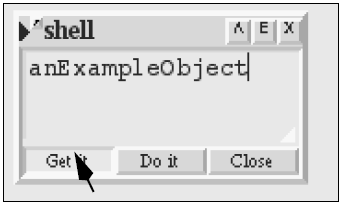
\includegraphics{Pgm_Env_Image2.png}}
\end{flushleft}\end{figure}

The result object appears in your “hand” raised above the screen as if you were dragging it with the
left button. Just click the button to set it down.
\begin{figure}[htbp]\begin{flushleft}

\scalebox{1.000000}{
\includegraphics{Pgm_Env_Image3.png}}
\end{flushleft}\end{figure}

As with most other things on the Self screen, the left button picks it up and moves it. (For buttons
and other things that use left-button for other purposes, you can grab them with marquee selection
(really the \emph{carpet morph} in Self) or with the “Grab” item on the right-button menu.)


\subsubsection{Expand and Collapse}
\label{howtoprg:expand-and-collapse}
Left-click on the triangle \footnote{
Double-clicking on the triangle will expand (or contract) all levels instead of just a single level. (This feature was added in Self 4.1.2.)
} to expand the object and see more information:
\begin{figure}[htbp]\begin{flushleft}

\scalebox{1.000000}{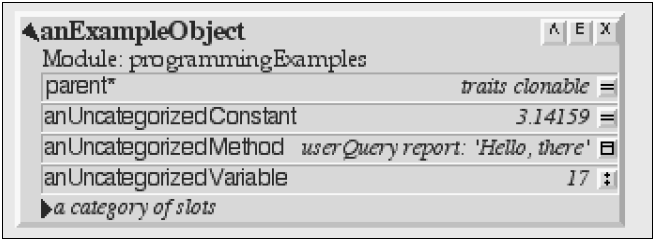
\includegraphics{Pgm_Env_Image4.png}}
\end{flushleft}\end{figure}

Now it shows a summary of modules containing the slots in this object (just \code{programmingExamples}
here), four slots, and a category containing more slots, although those slots are not shown
yet.


\subsubsection{Categories}
\label{howtoprg:categories}
Clicking the top triangle now would collapse this object outliner, but instead look inside the category
by clicking its triangle:
\begin{figure}[htbp]\begin{flushleft}

\scalebox{1.000000}{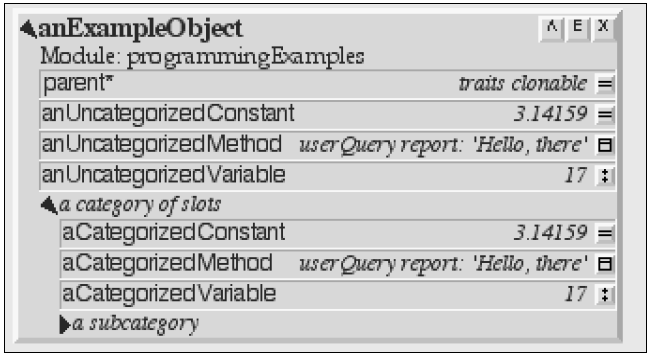
\includegraphics{Pgm_Env_Image5.png}}
\end{flushleft}\end{figure}

And, one more click expands the subcategory:
\begin{figure}[htbp]\begin{flushleft}

\scalebox{1.000000}{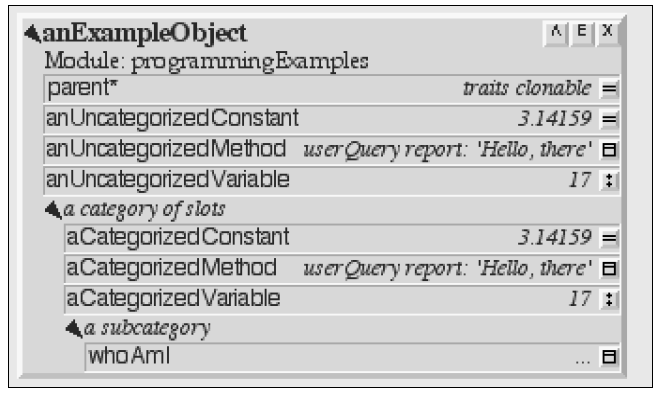
\includegraphics{Pgm_Env_Image6.png}}
\end{flushleft}\end{figure}


\subsubsection{Slots}
\label{howtoprg:slots}
The little icons on the right edges of the slots reveal the type of slot: 
\includegraphics{methodslot.png} for a method slot (a slot
containing a method), 
\includegraphics{constantslot.png} for a constant slot (a slot containing a data object), and 
\includegraphics{assignableslot.png} for an assignable
slot (a pair of slots containing a data object and the assignment primitive). In order to save
space, the data slot and its corresponding assignment slot are lumped together. (In other words in
addition to the visible slot named \code{aCategorizedVariable} containing 17, there is another, \emph{invisible}
slot named \code{aCategorizedVariable}: containing the assignment primitive.)

To look at the object contained in a data (constant or assignable) slot, just click on its icon. But if
the slot is a method, clicking its icon opens up a text editor on its source. For example, clicking on
the icon at the right of the whoAmI box opens a text editor displaying its source (and typing control-
L widens the object to show all the text in the selected window):
\begin{figure}[htbp]\begin{flushleft}

\scalebox{1.000000}{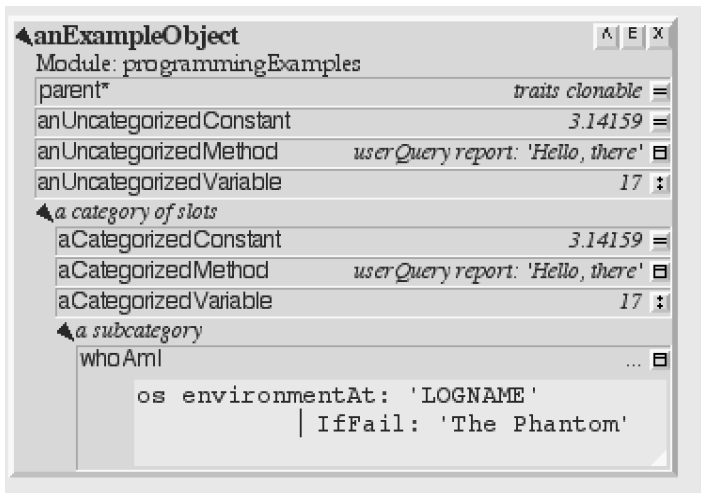
\includegraphics{Pgm_Env_Image7.png}}
\end{flushleft}\end{figure}


\subsubsection{Text Editors}
\label{howtoprg:text-editors}
The background of the editor is lighter than the outliner as a whole, and this difference indicates
that this editor is the current typing focus: no matter where the mouse is you can type into this editor.
A left-click on another editor will select that one as the typing focus, and to indicate that it is
no longer the focus, this editor’s background will change to match the outliner:
\begin{figure}[htbp]\begin{flushleft}

\scalebox{1.000000}{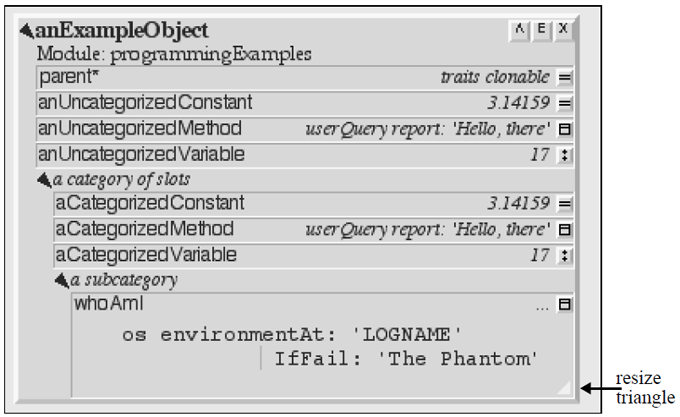
\includegraphics{Pgm_Env_Image8.png}}
\end{flushleft}\end{figure}

The white triangle in the lower-right corner of the editor (which can barely be seen in the printout
of this document) can be dragged to resize the editor.

Someone has done a poor job of indenting this method, so fix it by clicking to the left of the capital–
I and deleting two spaces:
\begin{figure}[htbp]\begin{flushleft}

\scalebox{1.000000}{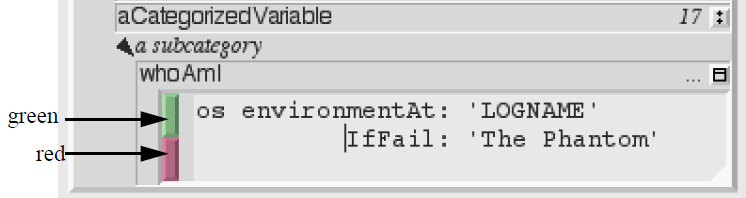
\includegraphics{Pgm_Env_Image9.png}}
\end{flushleft}\end{figure}

The red and green buttons that just appeared indicate the text has been changed; it no longer reflects
the source code of the real method. Hitting the red button will cancel the changes, while hitting
the green button will accept them and change the method:
\begin{figure}[htbp]\begin{flushleft}

\scalebox{1.000000}{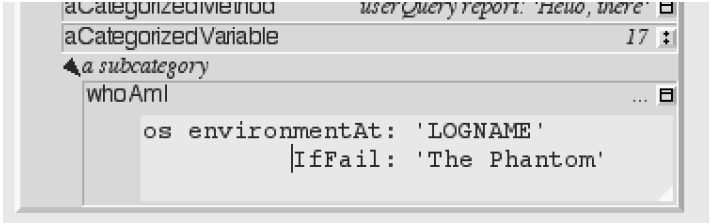
\includegraphics{Pgm_Env_Image10.png}}
\end{flushleft}\end{figure}

Self text editors will honor the cursor arrow keys, the copy, paste, and cut Sun keys, and
many emacs-style control characters:

\textbf{Table 1 Partial list of control characters in Self text editors}
\begin{quote}

\begin{tabulary}{\linewidth}{|L|L|}
\hline
\textbf{
Character
} & \textbf{
Effect
}\\\hline

control-a
 & 
move to start of line
\\\hline

control-b
 & 
back one character
\\\hline

control-d
 & 
delete next character
\\\hline

control-e
 & 
go to end of line
\\\hline

control-f
 & 
forward one character
\\\hline

control-k
 & 
kill to end of line
\\\hline

control-l
 & 
expand the text editor to show the whole text
\\\hline

control-n
 & 
go to next line
\\\hline

control-o
 & 
open a new line after the cursor
\\\hline

control-p
 & 
go to previous line
\\\hline

control-t
 & 
transpose characters
\\\hline

control-w
 & 
erase previous word
\\\hline

control-y
 & 
yank text from past-buffer to editor
\\\hline

delete, backspace, or control-h
 & 
erase-last-character
\\\hline

meta-return (command-return on Mac)
 & 
accept
\\\hline

escape (also command-period on Mac)
 & 
cancel
\\\hline

meta-s (command-s on Mac)
 & 
save a snapshot
\\\hline

meta-x (command-x on Mac)
 & 
cut
\\\hline

meta-c (command-c on Mac)
 & 
copy
\\\hline

meta-v (command-v on Mac)
 & 
paste
\\\hline

meta-d (command-d on Mac)
 & 
dismiss morph containing typing focus
\\\hline
\end{tabulary}

\end{quote}


\subsubsection{Dismissing Objects}
\label{howtoprg:dismissing-objects}
There are four separate ways of dismissing an outliner (or for that matter, anything) from the Self
desktop:
\begin{itemize}
\item {} 
Object outliners: Push the “X” button at the top-right-hand corner.

\item {} 
Drag it to the trash: left-drag on the outliner till the mouse is over the trash can, \raisebox{-0.5\height}{
\includegraphics{trashcan.png}} then release the mouse-button.

\item {} 
Dismiss it via the right-button menu: hold down the right button over the outliner, move to the Dismiss button, then release.

\item {} 
The Carpet Morph: start above (or below) and to the left (or to the right) of the outliner, over the background. Hold down the left button and sweep out an area that completely contains the outliner, then release the left button. The outliner should now be surrounded by a rectangle. Use the middle mouse button inside the rectangle to select \code{Dismiss}.

\end{itemize}

The last two methods, dismissing from the right-button menu, and marquee selection with the carpet
morph, come in especially handy with things like buttons and menus because such morphs cannot
be grabbed with the left-button.


\subsection{Menus in the Outliner}
\label{howtoprg:menus-in-the-outliner}
Many other operations are available on the outliner by using the middle-button menu on the part of
the outliner to be affected. For example anExampleObject has many regions and here are some
of them:
\begin{figure}[htbp]\begin{flushleft}

\scalebox{1.000000}{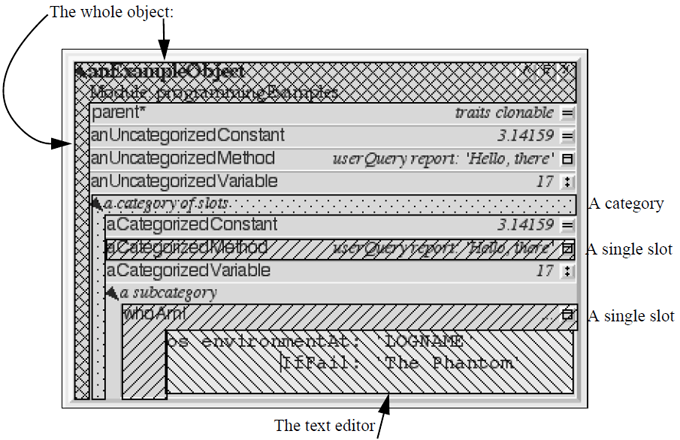
\includegraphics{Pgm_Env_Image11.png}}
\end{flushleft}\end{figure}

Click on the desired part of the object, be it object, category, slot, text editor, or annotation (annotations
will be explained later).


\subsubsection{The Evaluator}
\label{howtoprg:the-evaluator}
Try out the \code{whoAmI} method. Push the “E” button in the top-right of the outliner:
\begin{figure}[htbp]\begin{flushleft}

\scalebox{1.000000}{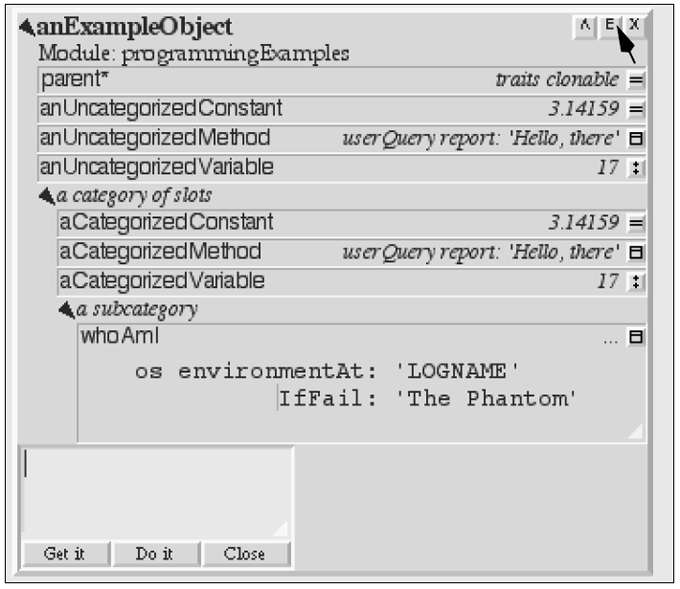
\includegraphics{Pgm_Env_Image12.png}}
\end{flushleft}\end{figure}

The receiver of any messages sent from an evaluator, or indeed any text editor (via \code{Do It} and \code{Get It}
in the editor’s middle-button menu) in an object outliner is the object itself. \footnote{
However, in a stack frame in the debugger (described below), the receiver of a message is the same as the receiver for the stack frame.
} Type \code{whoAmI} into
the evaluator and hit the Get it button (or select the Get It from the text editor menu), to send
the message and get back the result:
\begin{figure}[htbp]\begin{flushleft}

\scalebox{1.000000}{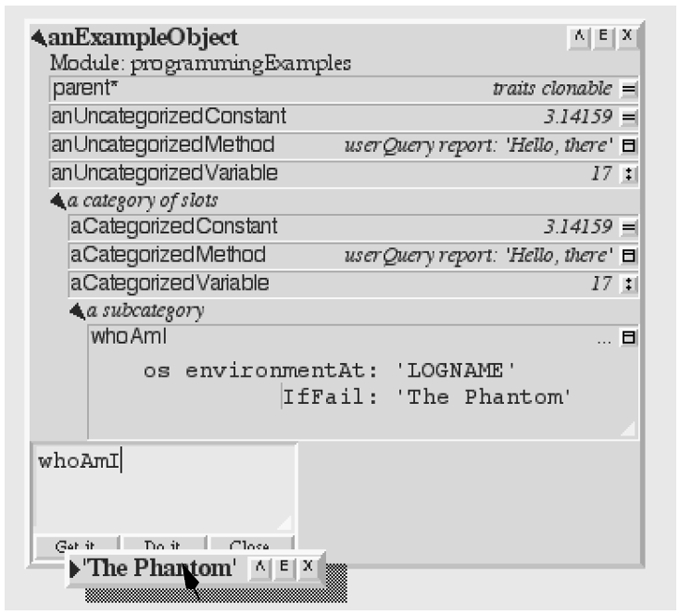
\includegraphics{Pgm_Env_Image13.png}}
\end{flushleft}\end{figure}

Move the result \footnote{
I am revising this for Self 4.1 on my trusty Mac, and Self does not implement environment variables here.
} out of the way and left-click to set it down.


\subsubsection{Adding a slot}
\label{howtoprg:adding-a-slot}
Try one more change: adding a slot to the category “\code{a category of slots}.” Hold the cursor
over the words a \code{category of slots} and select \code{Add Slot} from the middle-button menu.
\begin{figure}[htbp]\begin{flushleft}

\scalebox{1.000000}{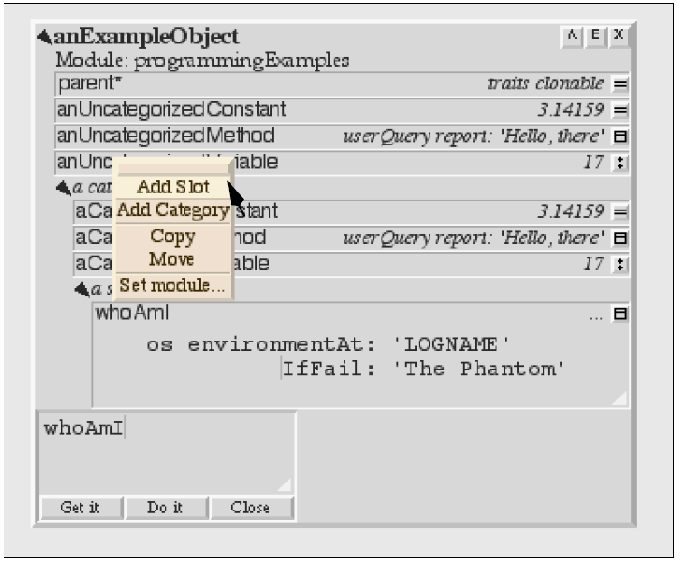
\includegraphics{Pgm_Env_Image14.png}}
\end{flushleft}\end{figure}

After selecting Add Slot a space for a new slot will appear in the object:
\begin{figure}[htbp]\begin{flushleft}

\scalebox{1.000000}{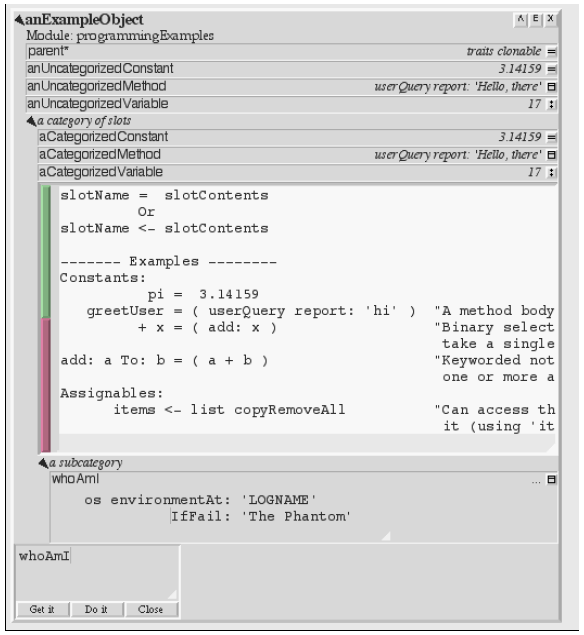
\includegraphics{Pgm_Env_Image15.png}}
\end{flushleft}\end{figure}

Each line shows the syntax for a different kind of slot. Create a simple variable by typing
\code{me\textless{}-’Gumby’} \footnote{
Since all that stuff in the text editor was initially selected, your typing conveniently replaced it all.
} and hitting the green button to accept the change:
\begin{figure}[htbp]\begin{flushleft}

\scalebox{1.000000}{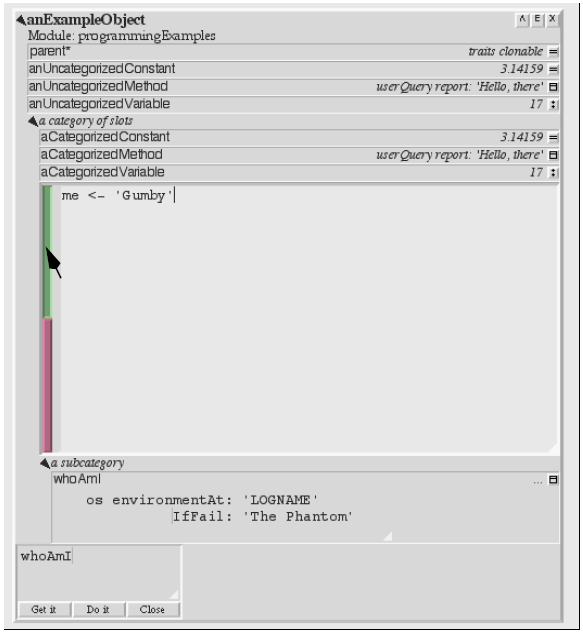
\includegraphics{Pgm_Env_Image16.png}}
\end{flushleft}\end{figure}

After releasing the green button, it stays down to let you know that it is still working. After a few
seconds the slot appears: \footnote{
If you examine the slot’s annotation (available via the slot menu) it will show that the system has guessed that the new slot (named “me”) should be saved in the “programmingExamples” module, and that instead of saving its actual contents, the slot should just be initialized to the string ‘Gumby’.
}
\begin{figure}[htbp]\begin{flushleft}

\scalebox{1.000000}{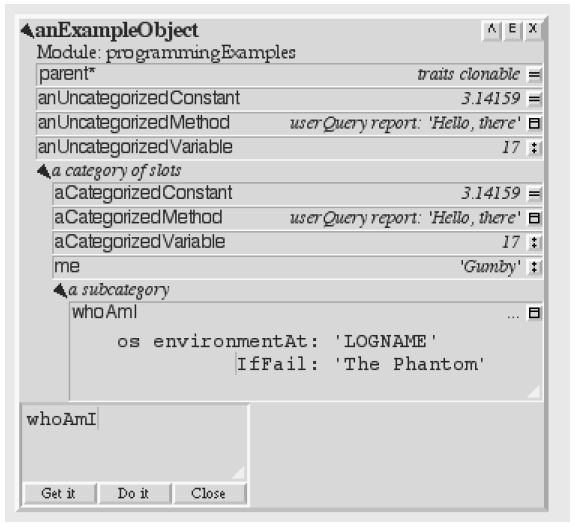
\includegraphics{Pgm_Env_Image17.png}}
\end{flushleft}\end{figure}


\subsection{Debugger}
\label{howtoprg:debugger}
Explore the Self debugger. Start by scrambling the send to \code{environmentVariable:IfFail} as
if you had misspelled it.
\begin{figure}[htbp]\begin{flushleft}

\scalebox{1.000000}{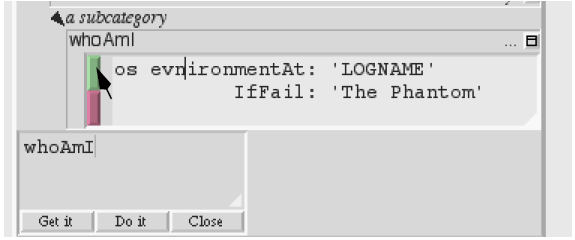
\includegraphics{Pgm_Env_Image18.png}}
\end{flushleft}\end{figure}

Press the green button to accept the change, then hit the \code{Get it} button. This should break something!
In fact, instead of the result of the message, a Self debugger will materialize:
\begin{figure}[htbp]\begin{flushleft}

\scalebox{1.000000}{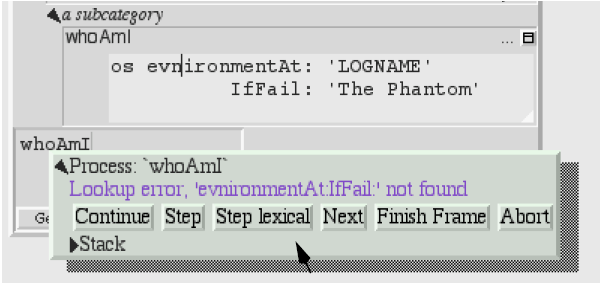
\includegraphics{Pgm_Env_Image19.png}}
\end{flushleft}\end{figure}

The debugger has a label to indicate which process ran aground, a status indication shown in blue,
some buttons for controlling the process, and a collapsed outliner for the stack. Expand the stack:
\begin{figure}[htbp]\begin{flushleft}

\scalebox{1.000000}{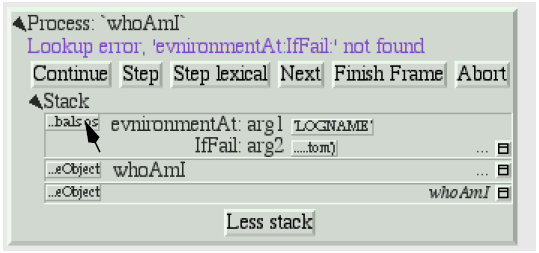
\includegraphics{Pgm_Env_Image20.png}}
\end{flushleft}\end{figure}

The stack filters out uninteresting frames by default. \footnote{
Since the Self compiler inlines calls automatically, Self code tends to be written in a highly-factored, deeply-nested style. Thus, the debugger filters out stack frames that seem to be unimportant. If it ever filters out the frame you need to see, there is a “Don’t filter frames” entry in the stack’s middle-button menu.
} The debugger assumes that the first method
you want to see is the one based on the text in the evaluator, and since the stack grows upwards this
oldest frame appears at the bottom. It has no method name, and contains the code \code{whoAmI}. That
method called \code{whoAmI}, whose code is too long to show next to the slot button, and that method
called \code{evnironmentAt:IfFail:} because we just sabotaged it! Of course there is no such method,
but Self creates one dynamically to handle the error.

The little boxes represent the receiver and arguments of the methods on the stack. Get the receiver
of the evnironment... message. Click on the box to the left of the word \code{evnironmentVariable:}
(the one labelled “\code{...bal os}” if you are running on the Macintosh):
\begin{figure}[htbp]\begin{flushleft}

\scalebox{1.000000}{
\includegraphics{Pgm_Env_Image21.png}}
\end{flushleft}\end{figure}

This object represents the interface to the Macintosh operating system. The little button with the
apostrophe in the top-left-hand corner indicates that this object has a comment. Push the button to
show (or hide) the comment:
\begin{figure}[htbp]\begin{flushleft}

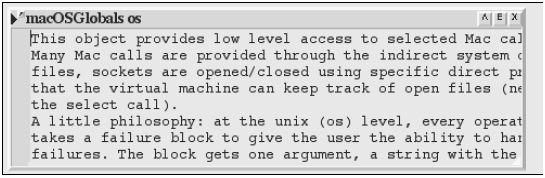
\includegraphics{Pgm_Env_Image22.png}
\end{flushleft}\end{figure}

(To automatically resize the outliner to show all the text, press control-L.) To see one of Self’s
scroll bars, grab the comment’s resize triangle (with the left-button) and move it up a bit:
\begin{figure}[htbp]\begin{flushleft}

\scalebox{1.000000}{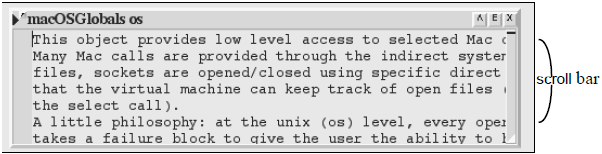
\includegraphics{Pgm_Env_Image23.png}}
\end{flushleft}\end{figure}

The affordance that appears on the right of the text is the scroll bar, and you can either drag on the
little black line or just click in the bar to scroll the text up or down.

Push the little apostrophe button again to hide the comment. Now, you could expand this object to
find the correct spelling of the evnironment... message. But instead, pretend that all you remember
is that it has the word “Variable” in it somewhere. So, use a facility called \code{Find Slot} that takes
a pattern and an object, and finds any matching slots in that object or its parents. Use the middlebutton
on the outliner’s title (\code{macOSGlobals os}) to get the object menu and select \code{Find slot}...
\begin{figure}[htbp]\begin{flushleft}

\scalebox{1.000000}{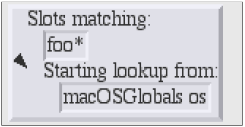
\includegraphics{Pgm_Env_Image24.png}}
\end{flushleft}\end{figure}

Double-click on the word “foo” to select that field for editing. (The same trick works on slot
names)
\begin{figure}[htbp]\begin{flushleft}

\scalebox{1.000000}{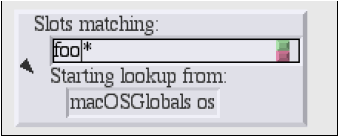
\includegraphics{Pgm_Env_Image25.png}}
\end{flushleft}\end{figure}

Since we are searching for a method with “Variable” in its name, backspace (the delete key on the
Mac) three times \footnote{
One rough edge remaining in the Self user interface is the existence of two test editors, and this one does not implement multi-character selection, sigh. Or, you could type control-A to go the start, and control-K to delete the whole field, sigh.
} to erase the “foo” type in *{}`{}`Variable{}`{}`*, hit the green button, and then hit the
triangle to start the search (if you make a typing mistake, you can double click the text to make it
editable again). The triangle will blink a bit while it is searching (one could do other things in the
meantime during a long search), then the enumerator will show the match(es):
\begin{figure}[htbp]\begin{flushleft}

\scalebox{1.000000}{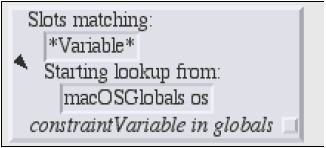
\includegraphics{Pgm_Env_Image26.png}}
\end{flushleft}\end{figure}

Clicking on the little square button(s) would show the exact method(s). But, for our purposes, just
knowing the name is enough and now you have to fix it. So back to the debugger and click on the
method button on the right in the \code{whoAmI} slot to expand the stack frame for the \code{whoAmI} method:
\begin{figure}[htbp]\begin{flushleft}

\scalebox{1.000000}{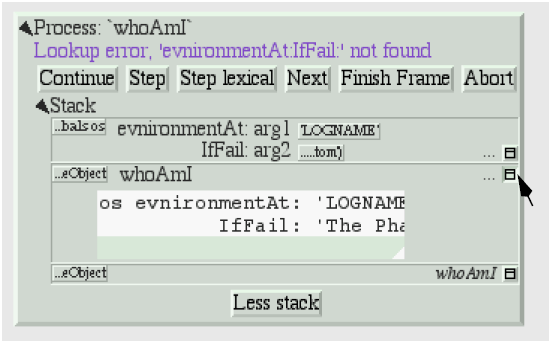
\includegraphics{Pgm_Env_Image27.png}}
\end{flushleft}\end{figure}

Now the debugger shows the source of the method, with the actual message being sent highlighted.
(In this case it is just the whole thing.) One of the conveniences in the Self programming environment
is that you do not have to go back to the original method to fix it, but can just fix it here (following
the grand tradition of Lisp and Smalltalk programming environments). So use the left
button to select the “vn” and type “nv” instead, then hit the green button to accept the change. The
green button will stay in a bit longer because when a method is changed from the debugger, every
slot pointing to that same method is made to feel the change—the method is changed in place (see
the figure below). This feature lets you change a method in a clone and simultaneously affect the
\begin{quote}
\begin{figure}[htbp]\begin{flushleft}

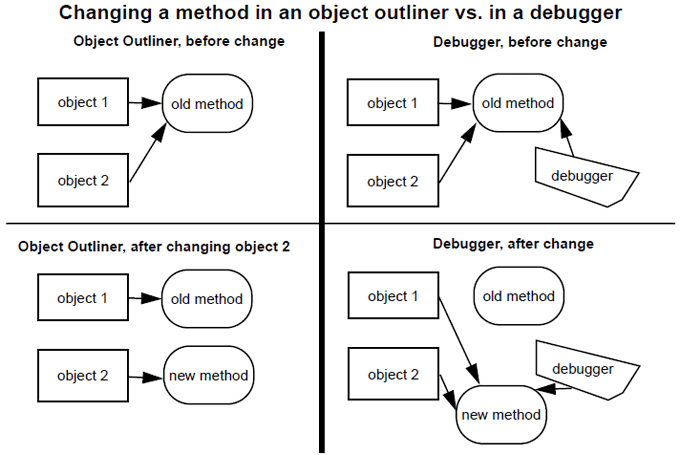
\includegraphics{Pgm_Env_Image28.png}
\end{flushleft}\end{figure}
\end{quote}

prototype, if you are putting your methods in prototypes instead of traits. Changing a method in an
ordinary outliner would just affect that one object, even if other objects had been cloned from it.
This rule avoids unintentional changes. The more global kind of change performed by the debugger
takes a little longer. When it is accomplished, the red and green buttons will disappear:
\begin{figure}[htbp]\begin{flushleft}

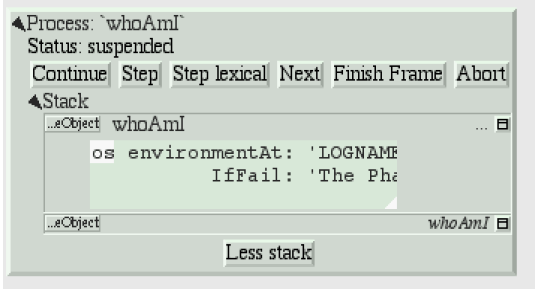
\includegraphics{Pgm_Env_Image29.png}
\end{flushleft}\end{figure}

Now os is highlighted to show that the process is about to send “os” to implicit-self. Try the \code{Step}
button, which performs a single message send. After hitting the \code{Step} button twice (and a control-
L to widen the debugger), the process will have entered the \code{environmentVariable:IfFail:} method:
\begin{figure}[htbp]\begin{flushleft}

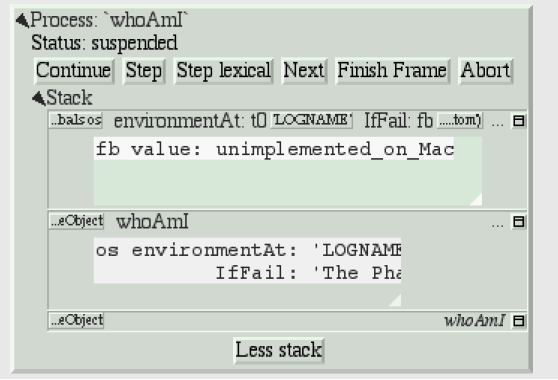
\includegraphics{Pgm_Env_Image30.png}
\end{flushleft}\end{figure}

This method is not too interesting (especially on the Macintosh), so leave the debugger by hitting
\code{Continue} and letting the process finish.

Congratulations on making through the interactive tutorial. In the remainder of this manual, we
will dive deeper into the programming environment for readers who want to write real programs in
Self.

Here is more information on the debugger for future reference:
\begin{quote}
\begin{quote}

\textbf{Table 2 The Debugger Buttons}
\end{quote}

\begin{tabulary}{\linewidth}{|L|L|}
\hline
\textbf{
What it says
} & \textbf{
What it does
}\\\hline

Continue
 & 
Resumes running the process
\\\hline

Step
 & 
Perform one message send (skipping over trivial accesses and assignments); Steps into the called method.
\\\hline

Step Lexical
 & 
Execute messages until control returns to the same lexical method, or until this method exits. Very useful for methods with blocks.
\\\hline

Next
 & 
Performs a message send and any messages in the called method; Steps over the called method.
\\\hline

Finish Frame
 & 
Finishes running the topmost method.
\\\hline

Abort
 & 
Kills off the process and dismisses the debugger.
\\\hline
\end{tabulary}

\end{quote}

In addition to the buttons, each frame in the debugger has some items to control the process in its
middle-button menu:
\begin{quote}
\begin{quote}

\textbf{Table 3 Process control items in the activation middle-button menu}
\end{quote}

\begin{tabulary}{\linewidth}{|L|L|}
\hline
\textbf{
What it says
} & \textbf{
What it does
}\\\hline

Step
 & 
Top frame: same as step button, not top frame: Finish any called methods.
\\\hline

Next
 & 
Same as next button.
\\\hline

Retry
 & 
Cut back the stack to this frame, then continue the process.
\\\hline

Revert
 & 
Cut back the stack to this frame.
\\\hline

Finish
 & 
Finish this frame.
\\\hline
\end{tabulary}

\end{quote}


\subsection{Enumerators}
\label{howtoprg:enumerators}
In addition to the \code{Find Slot} enumerator, Self has other ways to find things:
\begin{quote}

\textbf{Table 4 Enumerators}
\end{quote}

\begin{tabulary}{\linewidth}{|L|L|}
\hline
\textbf{
Name
} & \textbf{
Function
}\\\hline

Implementors
 & 
Finds all the slots with a given name.
\\\hline

Implementors of :
 & 
Finds all the slots with the given name that take an argument (for read/write slots only).
\\\hline

Senders
 & 
Finds all the methods that send a message with a given name.
\\\hline

Senders of :
 & 
Finds all the methods that send the corresponding assignment message (read/write slots only).
\\\hline

Senders in family (Senders of : in family)
 & 
Finds all the methods in this object, its ancestors, and descendants that send a message with a given name (or the corresponding assignment message).
\\\hline

Find Slot
 & 
Starting from a designated object, finds all slots in that object and its ancestors whose name matches a given pattern. Case is ignored, “?” matches any character, “*” matches any series of zero or more characters. Also comes in “of :” and “in family” flavors.
\\\hline

Methods Containing
 & 
Finds methods containing the specified string. Similar to grep without wildcards.
\\\hline

Copied-down Children
 & 
Finds objects copied-down (see below) from this one.
\\\hline

References
 & 
Finds slots that contain references to the selected object.
\\\hline

Slots in Module
 & 
On the module menu (see below); shows all slots in a given module.
\\\hline

Added or Changed Slots in Module
 & 
On the module menu (see below); shows all slots added or changed in the module since it was filed out.
\\\hline

Removed Slots in Module
 & 
On the module menu (see below); shows the names of the slots removed from the mod-ule since it was last filed out.
\\\hline

Expatriate Slots
 & 
On the changed module menu (see below); shows all slots in filed-out objects that do not themselves specify a module. These slots will not be filed out.
\\\hline
\end{tabulary}


The \code{copy-down} and \code{module} enumerators will be covered later.

The other enumerators can be summoned from several places: the outliner menu, the slot menu,
and the text editor menu. As a shortcut, selecting a whole expression in the text editor and then asking
for an enumerator will bring up the enumerator to search for the outermost message send in the
expression. So if you select the following expression: \code{aSet} \code{findFirst:} \code{elem IfPresent:}
\code{{[}snort{]}} \code{IfAbsent:} \code{{[}sludge{]}} and choose implementors from the text editor menu, you will
get an Implementors enumerator ready to search for \code{findFirst:IfPresent:IfAbsent:}. Of
course, you can always change the search target by double-clicking and editing the text. The text
editors also implement a host of handy double-clicking shortcuts.

Finally there is one last detail about enumerations: many contain a check-box to choose \code{Wellknown
only}. This is always checked by default to speed things up. When checked, only wellknown
(i.e. filed-out, see below) objects are searched, which is much faster.


\section{Hacking Objects}
\label{howtoprg:hacking-objects}
\emph{Hacking---the discipline of making fine furniture from trees using an axe.}

In going through this document, you have already added a slot and edited methods in both object
outliners and debuggers. In addition Self 4.1 has many other ways to change an object:
\begin{quote}

\textbf{Table 5 Ways to change an object}
\end{quote}

\textbf{Removing, Moving, Copying Categories}

\begin{tabulary}{\linewidth}{p{5cm} p{5cm} p{5cm}}
\hline
\textbf{
Ways to change an object
} & \textbf{
How
} & \textbf{
Why
}\\\hline
 & 
\textbf{Removing, Moving, Copying Categories}
 & \\\hline

Removing a category.
 & 
“Move” in category middle menu, then drag the category to the background or the trash can.
 & 
Removing a category
\\\hline

Add slot or category to object or category.
 & 
“Add Category” in object or category middle menu, then type in the new category name, then hit green button to accept.
 & 
Adding a new category.
\\\hline

Moving a category.
 & 
“Move” in category middle menu, then drag to another object.
 & 
Copying a category.
\\\hline

Copying a category.
 & 
“Copy” in category or category middle menu, then drag the category to another object.
 & 
Copying a category.
\\\hline
\end{tabulary}


\begin{tabulary}{\linewidth}{p{5cm} p{5cm} p{5cm}}
\hline
 & 
\textbf{Removing, Adding, Moving, Copying Slots}
 & \\\hline

Removing a slot.
 & 
“Move” in slot middle menu, then drag the slot to the background or the trash can.
 & 
Removing a slot
\\\hline

Add slot to object or category
 & 
“Add Slot” in object or category middle menu, then type in the new slot name, “=” or “\textless{}-”, and contents of slot (or just name alone for variable slot containing nil), then hit green button to accept.
 & 
Adding adding a new
\\\hline

Moving a slot.
 & 
“Move” in slot middle menu, then drag to another object.
 & 
Moving a slot.
\\\hline

Copying a slot.
 & 
“Copy” in slot or category middle menu, then drag the slot to another object
 & 
Copying a slot.
\\\hline
\end{tabulary}


\begin{tabulary}{\linewidth}{p{5cm} p{5cm} p{5cm}}
\hline
 & 
\textbf{Changing a slot}
 & \\\hline

Edit a slot
 & 
“Edit” on a slot middle-button menu, then make any changes in the text editor, then hit green button to accept changes.
 & 
To change the contents of a constant data slot, or to change contents and set initial value at same time, or to change a slot from data to method or from constant to variable.
\\\hline

Edit slot name or its argument names
 & 
Double-click on the name of the slot, wait for red and green buttons to appear on the right of the name, edit the name, then hit the green button.
 & 
To change a slot’s name or the names of its arguments.
\\\hline

Change a method in a slot.
 & 
Click on the method icon button on the right of the slot to open a text editor on the method. Make the changes, then click on the green button to accept them.
 & 
To fix a bug in a method.
\\\hline

Change the visibility of a slot
 & 
On the slot’s middle menu choose “Make Public,” “Make Private,” or “Make Undeclared.”
 & 
The Self interface uses bold, normal, and sans-serif fonts to indicate public, private, and unspecified slots.This distinction carries no semantics, but serves to record the programmer’s intentions.
\\\hline
\end{tabulary}


\begin{tabulary}{\linewidth}{p{5cm} p{5cm} p{5cm}}
\hline
 & 
\textbf{Adding a Comment}
 & \\\hline

Add a comment to an object or slot
 & 
“Show Comment” in the object or slot middle menu to open up a comment text editor, then typing in the comment, then hit the green button to accept it. If an object or slot already has a comment, it can be shown/hidden by hitting the
small button labeled with a single quote.
 & 
To amuse and intrigue those who follow
\\\hline
\end{tabulary}


\begin{tabulary}{\linewidth}{p{5cm} p{5cm} p{5cm}}
\hline
 & 
\textbf{Annotating an Object}
 & \\\hline

Change creator annotation of an object
 & 
“Show Annotation” in object middle menu to expose object annotation information, then click on creator path field and typing in desired creator path., then hit green button to accept annotation.
 & 
Setting creator path tells transporter which slot “owns” this object, and tells environment what to name the object.
\\\hline

Set creator of contents of a slot to that slot
 & 
“Set Creator” in slot middle menu.
 & 
See above.
\\\hline

Change copy-down information
 & 
“Show Annotation” in object middle menu to expose object annotation information, then click on copy-down-parent field and type in desired copy-down-path., copy-down selector and slots to omit) then hit green button to accept annotation.
 & 
Simulates subclassing by allowing an object to contain copies of the slots in another object. When copy-down-parent has slots added/ changed/removed, the change propagates to the copied-down children.
\\\hline

Change the object’s “isComplete” flag
 & 
“Show Annotation” in object middle menu to expose object annotation information, then push one of the isComplete radio buttons, then hit green button to accept the annotation change.
 & 
After building a new prototype, set isComplete to get the environment to show its printString, and to get the transporter to use its storeString.
\\\hline
\end{tabulary}


\begin{tabulary}{\linewidth}{p{5cm} p{5cm} p{5cm}}
\hline
 & 
\textbf{Annotate a slot}
 & \\\hline

Set the module memmbership of a slot, the slots in a
category, or the slots in an object.
 & 
Select “Set Module” from the middle menu of a slot, category, or object, then (for object or category) indicate which slots you want to change by choosing which module they currently belong to, finally select a
new module to put the slots in
 & 
To ensure that slots are filled out in the correct source file
\\\hline

Type in or examine the module for a single slot
 & 
“Show Annotation” on the slot middle menu to expose the annotation, then click on the module editor, type in the module name, then click the green accept button.
 & 
Save as above.
\\\hline

Change slot initial contents
 & 
“Show Annotation” on the slot middle menu to expose the annotation, then click on the “Follow Slot” button, or type the desired initial value expression into the ‘Initial Con-tents” editor, then hit the green accept button.
 & 
To have the transporter record the current contents of a slot, choose “Follow Slot.” To have it ignore the current value and just record a given expression for the slot’s initial value use the “Initial Contents” option.
\\\hline
\end{tabulary}



\section{The Transporter}
\label{howtoprg:the-transporter}
The transporter has been built in order to move programs from one world of objects to another. so,
you can ignore it as long as you work with just one snapshot. However, if you want to give your
program to someone else, or save it as source, or read it in to a newer snapshot, you will need to
learn about the transporter.


\subsection{The Traditional Schism between Program and Data}
\label{howtoprg:the-traditional-schism-between-program-and-data}
What is a program? In most systems it is a piece of text, although in more advanced environments
it may have structure. It is a description that can be used to create an activity, a running program,
that can then operate on data. In the conventional view:
\begin{quote}

\textbf{Table 6 The Schism between Program and Data}

\begin{tabulary}{\linewidth}{|L|L|L|}
\hline
\textbf{} & \textbf{
Program
} & \textbf{
Data
}\\\hline

Who can change it
 & 
The programmer
 & 
The user
\\\hline

When can it change
 & 
At programming time
 & 
At execution time
\\\hline

How is it changed
 & 
With a text editor
 & 
By running a program
\\\hline
\end{tabulary}

\end{quote}

This model grew up in an era where computers were too small to host both compilers and applications
at the same time. Although it has some virtues it makes other operations very hard: it is hard
to include data, such as hand-drawn icons, directly into a program, and it is hard to write applications
whose data domain is really programs.


\subsection{Data = Program}
\label{howtoprg:data-program}
For Self, we have gone a different way, following in the footsteps of Smalltalk and Lisp:
\begin{quote}

\emph{A Self program consists of live objects.}
\end{quote}

Self has no edit/run mode. To change an object, you do not retreat to a source file, or even to a class,
you just change the object itself. This immediacy and concreteness lessens the cognitive burden on
the programmer, smooths the learning curve, and hastens gratification.

However, this stance creates a big problem the moment you need to move a program from one
world of objects to another; it is very hard to pin down what to do. For example, suppose an object
contains a slot with 1024 in it. Should that value be copied literally? Perhaps it is the result of some
computation (such as the width of the current screen) and should be recomputed instead. There
simply is not enough information in a Self object to extract programs from Snapshots.


\subsection{Changes vs. Pieces}
\label{howtoprg:changes-vs-pieces}
Earlier in the project we considered constructing a calculus of changes that could be used to represent
programs, and then moving programs by reapplying the changes to the new snapshot. But, we
had enough on our plate and rejected this approach as too ambitious to tackle without a dedicated
graduate student.

Instead, we decided to represent programs as pieces that could be filed out of a snapshot and filed
in to another. To allow us to merge changes to the same program, we decided to represent its pieces
as Unix source files amenable to RCS. The Self Transporter was built to save programs as source
files.


\subsection{Objects vs. Slots}
\label{howtoprg:objects-vs-slots}
But what is a program? Although a new program frequently involves creating new objects, it also
can mean added slots to existing objects. For example, a program to find palindromes might add a
slot to \code{traits string} called \code{isPalindrome}. So we decided to refine the granularity of the
Transporter to the slot level; each slot has an annotation \footnote{
The Self Virtual Machine provides for annotations on slots or whole objects. While the annotations do not influence program execution, they can be accessed and modified by Self’s reflective facility, mirrors. Annotations are used to hold many things, including comments on objects and slots.
} (its module) which gives the name of the
source file containing that slot. This hair- or rather object-splitting implies that one object may be
built incrementally as the result of reading several files, and so the transporter endeavors to keep
the order that the files are read in as independent as possible. Since each object can possess slots
in different modules, the outliner shows a summary of the modules of an object, sorted by frequency.

Turned around, a module can be viewed as a collection of slots, plus some other information: each
module also includes a directory, a list of submodules to be read in whenever it is read, and
\code{post-FileIn} method to be run whenever the module is read. These data allow modules to be organized
hierarchically by subsystem, for example the allUI2 module includes all the modules in the ui2
system.

Now here comes the nice part: the Self environment incrementally maintains a mapping from modules
to slots, and a list of changed modules, which can be obtained from the background menu.
When you make a change the appropriate module will be added to the list, and can be written as a
source file by clicking its w button. The middle-button menu on the changed modules and individual
modules contains a host of useful entries for understanding what has been changed.


\subsection{What to Save for the Contents of a Slot}
\label{howtoprg:what-to-save-for-the-contents-of-a-slot}
At this point, the reader may be thinking “So modules know which slots they include, but how do
they know which objects to include?” After all, when the transporter saves a slot in a file what can
it put for the contents of the slot? Here is where the transporter runs smack into the problem of not
enough information, and a variety of means have to be used. As shown in the flowchart below:
\begin{figure}[htbp]\begin{flushleft}

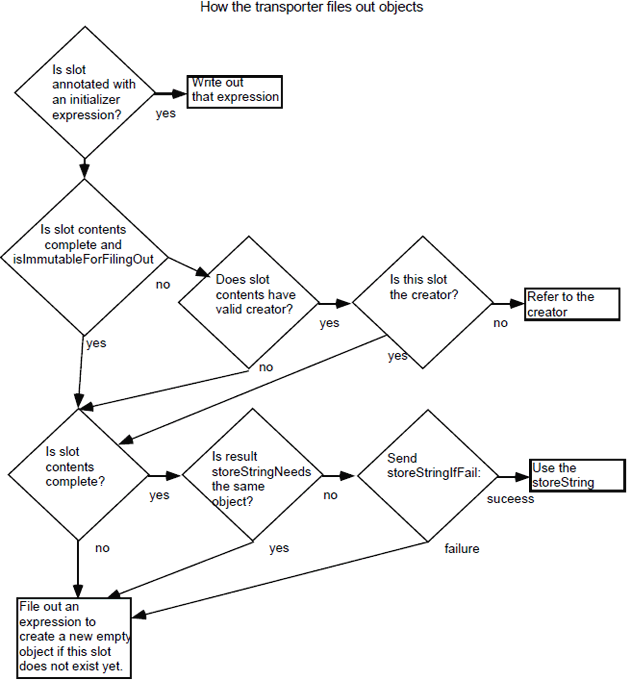
\includegraphics{Pgm_Env_Image31.png}
\end{flushleft}\end{figure}
\begin{itemize}
\item {} 
Sometimes the programmer does not want to store the actual contents of a slot, but instead
wants to store an initialization expression. This intention is captured with another annotation
on a slot: each slot can either be annotated \code{Follow Slot} or \code{Initialize To Expression}
In the latter case, an initializer is also supplied.

\item {} 
Even though the transporter is supposed to follow the slot, it may contain an object that is created
by another slot. For example, the \code{parent} slot in a point should just refer to \code{traits point}
rather than recreating the traits object. This information is captured by a \code{Creator} annotation
on each object that gives the path from the \code{lobby} to the slot intended to create the object.
In this case, the transporter just files out a reference to the object’s creator, cleverly
enough so that the actual creator slot does not need to have been already filed in. On the other
hand, if an object is immutable, its identity is not important. If an object is annotated as
\code{is-Complete} \footnote{
isComplete is used by the environment to decide when it is safe to send messages like printString.
} the transporter sends it \code{isImmutableForFilingOut} and if that message returns
\code{true}, the transporter never files out a reference. For example, integers would answer
\code{true} to this message.

\item {} 
If the contents of the slot is a simple (usually immutable) object like \code{17}, \code{3@4}, or ‘\code{foo}’ (the
string) the transporter should just ask the object for a string to store. It does this by checking to
see if the object is annotated as \code{isComplete} to see if it is safe to send the object messages,
checks to see if this object is itself needed for the string (it would be a mistake to file out the
prototypical point as \code{0@0}, because the x slot would never be defined), then asks the object for a
store string.To see if the object must itself be filed out, it sends \code{storeStringNeeds} and if
this message does not return the object itself it sends \code{storeStringIfFail}:. If this succeeds,
the transporter can save a data-type specific string for the object. This fairly elaborate mechanism
allows programmers to add new kinds of objects that transport out with type-specific creation
strings.

\item {} 
Finally, if it can do nothing else, the transporter creates a new object for the contents of the
slot. The object is created in a clever way so that a file that adds slots to an object can be read
before the file that officially creates the object without loss of information.

\end{itemize}

Filing out objects is too complicated, and over the past two years we have repeatedly tried simpler
schemes. However, all of the capabilities in the current scheme seem to be essential in some case.
This issue remains as a question for future work.


\subsection{Copy Down}
\label{howtoprg:copy-down}
Because Self eschews classes and because the current compiler cannot optimize dynamic inheritance,
it is necessary to copy-down slots when refining an object. For example, the prototypical
morph object contains many slots that every morph should have, and some mechanism is needed
to ensure that their presence is propagated down to more specialized morphs like the circleMorph.
In a class-based language, this need is met by a rule ensuring that subclasses include any instance
variables defined in their superclasses. In Self, this inheritance of structure is separated from the
inheritance of information performed by the normal hierarchy of parent slots. Instead of including
a facility for inheriting structure in the language, Self 4.1 implements a facility in the environment,
called “copy-down.” An object’s annotation can contain a copy-down parent, copy-down selector,
and set of slots to omit. The copy-down parent is sent the message given by the copy-down selector,
and (except for the slots-to-omit), the slots in the result are added to the object. Copied-down
slots are shown in pink in the outliner. For example, here are the prototypical morph and the prototypical
circleMorph:
\begin{figure}[htbp]\begin{flushleft}

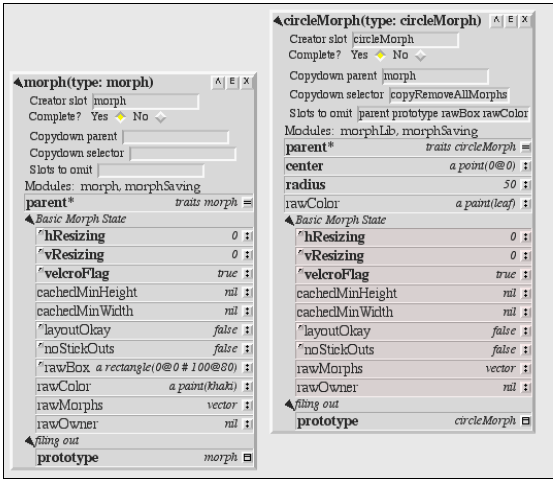
\includegraphics{Pgm_Env_Image32.png}
\end{flushleft}\end{figure}

The \code{Basic Morph State} category of slots has been copied from those in morph by first copying
the morph and removing all its submorphs (i.e. by sending it copyRemoveAllMorphs) and then
copying the resultant slots, omitting \code{parent}, \code{prototype}, \code{rawBox} and \code{rawColor}. The first
three of these slots were omitted because their contents had to be different; copied-down slots are
copied, they cannot be specially initialized in Self 4.1. The omitted slot \code{rawBox} is more interesting;
circle morphs do not need this slot at all and so omit it. Most other object-oriented programming
systems would not allow a subclass to avoid inheriting an instance variable.

The Self 4.1 programming environment uses the copy-down information to allow the programmer
to use a class-based style when appropriate. For example, if the programmer adds a slot to morph
the environment will offer to add it to \code{circleMorph}, too. If the programmer should use a text editor
to edit the definition of morph, the circleMorph object will be changed after rereading both object’s
text files. The least convenient aspect of using copy-downs is that to do the moral equivalent
of creating a subclass, the programmer has to create two objects: a new traits object, and a new prototype,
and then set the object annotation of the new prototype. Perhaps someday there will be a
button to do this, or perhaps other styles of programming will emerge.

This concludes a brief tour of the Self 4.1 programming environment. Although we strove for simplicity
in the design of Self, its programming environment includes a fair amount of functionality
which may take a while to learn. We hope that you find the investment worth the reward.
\paragraph{Footnotes:}


\chapter{Morphic: The Self User Interface Framework}
\label{morphic::doc}\label{morphic:morphic-the-self-user-interface-framework}

\section{Overview}
\label{morphic:overview}
Morphic is a user interface framework that supports composable graphical objects, along with the machinery required to display and animate these objects, handle user inputs, and manage underlying system resources such as X displays, fonts, and color maps. A primary goal of morphic is to make it easy to construct and edit interactive graphical objects, both by direct manipulation and from within programs.

A Morphic window shows just one portion of a large, two-dimensional world. The window can be panned around in this world, allowing different areas to be used for different activities. Multiple users can be active in this world simultaneously, working either in the same area (for collaborative work) or in disjoint areas (for independent work). Every user can see the screen boundaries, cursors, and actions of the other users. The sharing is implemented via the X protocol, so the other users can be physically remote as long as there is sufficient network bandwidth to support the X traffic. (Preliminary tests suggest that 30-50 KBytes/sec is required between the host machine and each remote user. The system has been tested with up to five users active simultaneously.) A given user can have several Morphic windows open, either on the same world or on different worlds, and can drag objects among these windows (assuming they all belong to the same Self Unix process).
\begin{figure}[htbp]\begin{flushleft}
\capstart

\scalebox{1.000000}{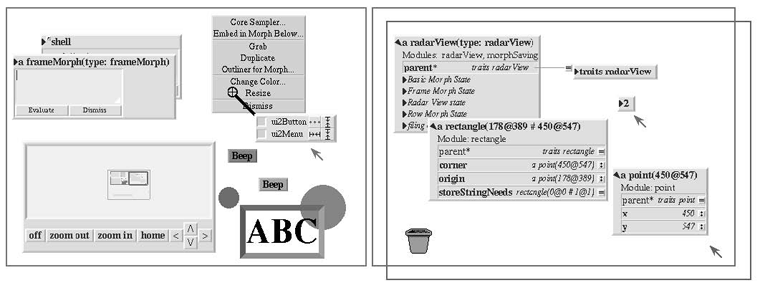
\includegraphics{Figure1.png}}
\caption{Figure 1: Three users working in the same space. Two of the other users are collaborating, so they have made their windows overlap (right). The third user is working independently in a separate area (left). The radarView in the third user's area shows the surrounding vicinity in miniature, allowing offscreen objects and the screen boundaries of other users to be seen. The radarView is updated open enough to see where activity is occurring.}\end{flushleft}\end{figure}

The central abstraction of morphic is the graphical object or \emph{morph} (from the Greek for ``shape'' or ``form''). A morph has a visual representation that can be picked up and moved. In addition, a morph may:
\begin{enumerate}
\item {} 
perform actions in response to user inputs,

\item {} 
perform an action when a morph is dropped onto it or when it is dropped onto another morph,

\item {} 
perform an action at regular intervals, and

\item {} 
control the placement and size of its submorphs.

\end{enumerate}

Any morph can have component morphs (called \emph{submorphs}). A morph with submorphs is called a \emph{composite} morph. A composite morph is treated as a unit; moving, copying, or deleting a composite morph causes all its submorphs to be moved, copied, or deleted as well. By convention, all morphs are visible; morphic does not use invisible structural morphs for aggregation. This means that if a composite morph is disassembled, all its component morphs can be seen and manipulated.

The remainder of this document discusses the graphics interface that morphs use to draw themselves, the structure of composite morphs, how to create new kinds of morphs, and how to change a morph's behavior with respect to user inputs, drag-and-drop, and animation.


\section{Composite Morphs}
\label{morphic:composite-morphs}
A \emph{composite} morph is a morph that contains other morphs known as \emph{submorphs}. Note that the terms ``composite'' and ``submorph'' refer to roles that can be played by any morph. Submorphs can be added to any kind of morph-even morphs such as circleMorphs or labelMorphs that are atomic in some other systems. Copying, deleting, moving, drawing, and layout operations are applied to the composite morph as a whole.

The structure of a composite morph forms a tree. When morph B is a submorph of morph A, B's \emph{owner} is A and B appears in A's \emph{submorphs} list. A morph can only be a submorph of at most one morph at a time, so its owner is a single value, not a collection. A window containing a collection of morphs is itself just a morph known as a \emph{worldMorph}. Each user's cursor is represented by a \emph{handMorph}. Grabbing a morph with the mouse is implemented by removing the target morph from the worldMorph and adding it to the handMorph. Dropping a morph when the mouse is released is implemented by reversing this process. A handMorph is itself a submorph of its world. The message \emph{root} can be sent to a morph to get the top-most owner of a composite morph (stopping just short of the worldMorph or handMorph that contains it). If a morph is not a submorph of any morph, its owner is \emph{nil}.
\begin{figure}[htbp]\begin{flushleft}
\capstart

\scalebox{0.800000}{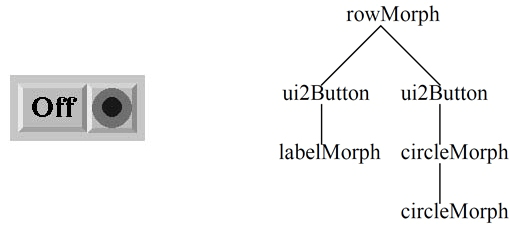
\includegraphics{Figure2.png}}
\caption{Figure 2: A composite morph consisting of a row with two buttons. Each button has submorph to indicate its function; one is a piece of text, the other is an icon consisting of two concentric circles. The diagram on the right shows its submorph structure.}\end{flushleft}\end{figure}

A morph can be made a submorph of some other morph using the \textbf{addMorph:} operation. This operation updates both the owner slot of the submorph and the submorphs list of the owner to reflect the desired configuration. For example, adding morph B to morph A adds B to A submorph list, removes B from its old owner (if any), and sets B's owner to A. The \textbf{addMorph:} operation also updates the layout of both B's old and new owners. The global position of a morph is held invariant by \textbf{addMorph:} (although some morphs may perform an automatic layout as a side-effect of \textbf{addMorph:}, immediately changing the position of the newly-added morph.).
\begin{figure}[htbp]\begin{flushleft}
\capstart

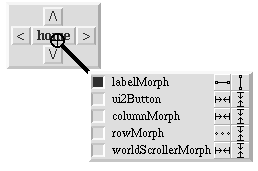
\includegraphics{Figure3.png}
\caption{Figure 3: Using the core sampler to probe the submorphs at the point below its cross-hairs.}\end{flushleft}\end{figure}

The programming environment includes a tool called the \emph{core sampler} (available via the right-button menu of any morph) that can be used to explore the submorph structure of a composite morph. The core sampler shows the set of submorphs below a given point, the way a core sample of rock allows geologists to study the strata of rock at a given point. The core sampler allows one to use the middle button menu to operate on morphs below the surface and can be used to insert or remove morphs from a composite morph. Holding the left mouse button over the squares along the left side of the core sampler highlights the associated morph. As a shortcut, holding down the shift key while pressing the left mouse button over one of these squares will extract the associated submorph (and all its submorphs) from the composite morph. Holding the shift key while dropping a morph onto one of these squares will insert the morph as a submorph of the associated morph. The iconic buttons on the right show the current resizing attributes of the associated morph, and allow them to be changed. (Resizing attributes are discussed in section 7.)


\section{Morph Traits and Prototypes}
\label{morphic:morph-traits-and-prototypes}
Morphic organizes morphs into a hierarchy much like a class hierarchy. The behavior for all ``instances'' of a given morph ``class'' is defined in a shared traits object which is a parent of all the instances. The structure of an instance is defined by the slots of its prototype. The root of the morph hierarchy is \textbf{traits morph}. All morphs inherit from \textbf{traits morph}, either directly or via one or more intermediate traits objects. (Note: to see the entire morph hierarchy, invoke the ``Show Traits Family'' menu command on an outliner on \textbf{traits morph} in the user interface. Be patient; the morph hierarchy is quite large.)

Usually, the prototype of a given morph contains all the slots of the morph from which it is derived (the ``instance variable of its superclass'' in a class-based system) plus, possibly, a few additions. To simplify the life of the programmer, the programming environment supports an idiom known as ``copying down.'' The derived prototype is described differentially. That is, it is ``just like its copy-down parent except with particular slots added, deleted, or changed.'' Typical class-based languages also describe the structure of subclasses differentially: a subclass may extend its superclass with additional instance variables. However, the copy-down idiom also allows the derived prototype to selectively omit slots of its copy-down parent or change their contents. For example, the circleMorph prototype is derived from the morph prototype, but it replaces the ``rawBox'' slot of the morph prototype with the slots ``radius'' and ``center''. This would not be possible in most class-based languages.

Note that the class-like organization of the morph hierarchy—with its parallel traits and prototype hierarchies and its use of the copy-down mechanism to propagate slot information down the prototype hierarchy—is only one way that Self programs can be organized. Other parts of the system, such as the world-wide-web browser, are organized differently.


\subsection{Implementing a New Kind of Morph}
\label{morphic:implementing-a-new-kind-of-morph}
It is easy to make a new kind of morph. One typically starts with a copy of some existing morph and adds or overrides state and behavior to create the new morph. Often, the most appropriate starting point is a copy of \emph{morph}, the root of the morph object hierarchy. Morph has default behavior for everything from drawing to handling user inputs; one thus starts with a working morph and modifies its behavior incrementally to create the new type of morph.

The programming aspect of creating a new morph is straightforward. However, four other things must be done to make the new morph into a first-class citizen. First, its behavior should be factored into a shared parent (called a traits object) to allow the behavior of all instances to be changed by changing the shared parent. Second, the shared traits object and a prototypical instance of the new morph should be embedded in the global namespace. Third, the copy-down parent of the prototype should be set so that changes to the structure of the parent are propagated correctly. Finally, the new prototype and traits objects should be assigned to a module to allow the code for the new morph to be saved in a file.

Of course, if one just wants to do a quick experiment, none of these housekeeping chores are necessary. However, sometimes one decides to make an experimental morph into a first-class morph (the bottom-up approach). In other cases, one sets out from the beginning to create a new first-class morph (the top-down approach). The next two sections will describe how to create a new kind of first-class morph using each of these approaches.


\subsection{Morph Creation: The Bottom-up Approach}
\label{morphic:morph-creation-the-bottom-up-approach}
In the bottom-up approach, one is initially interested in getting a morph with the desired behavior as quickly as possible. Thus, an appropriate morph is copied and modified by adding slots directly to the morph itself. Suppose one wished to create a morph that displayed as an oval and that toggled between two colors when the middle mouse button was pressed. To get a morph to modify, evaluate:
\begin{quote}

\begin{Verbatim}[commandchars=\\\{\}]
morph copy
\end{Verbatim}
\end{quote}

This will make an outliner on a new morph. Use the ``Show Morph'' command on this outliner's middle-button menu to make the graphic representation of the copy appear.

The ``Add Slot'' command on the outliner's middle-button menu can be used to add a data slot to hold the alternate color. Enter the following expression and accept it by clicking on the green (top) button:
\begin{quote}

\begin{Verbatim}[commandchars=\\\{\}]
otherColor \textless{}- paint named: 'leaf'
\end{Verbatim}
\end{quote}

The morph's drawing behavior can be customized by adding the method:
\begin{quote}

\begin{Verbatim}[commandchars=\\\{\}]
baseDrawOn: aCanvas = (
        aCanvas fillArcWithin: baseBounds
                From: 0
                Spanning: 360
                Color: color.
        self)
\end{Verbatim}
\end{quote}

Morphic optimizes shadow drawing for rectangular morphs such as prototypical morph, which draws as simple rectangle. However, this morph is not rectangular. To make its shadow reflect its true shape, the isRectangular behavior must be overridden by adding the constant slot:
\begin{quote}

\begin{Verbatim}[commandchars=\\\{\}]
\PYG{n}{isRectangular} \PYG{o}{=} \PYG{n}{false}
\end{Verbatim}
\end{quote}
\begin{figure}[htbp]\begin{flushleft}
\capstart

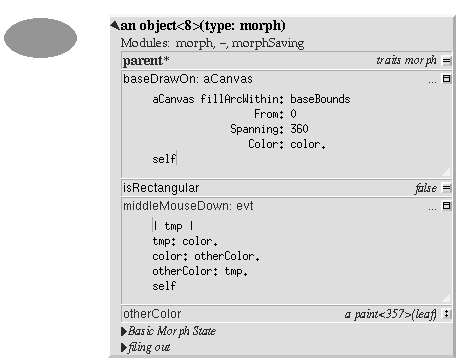
\includegraphics{Figure4.png}
\caption{Figure 4: A new kind of morph has been created by modifying a copy of the standard morph. The slots baseDrawOn:, isRectangular, middleMouseDown:, and otherColor have been added to the morph to obtain the new behavior. The morph itself appears on the left; an outliner showing its slots appears on the right.}\end{flushleft}\end{figure}

The new morph's input behavior can be customized by adding the method:
\begin{quote}

\begin{Verbatim}[commandchars=\\\{\}]
middleMouseDown: evt = (\textbar{} tmp \textbar{}
        tmp: color.
        color: otherColor.
        otherColor: tmp).
\end{Verbatim}
\end{quote}

The morph now draws itself as a filled oval. Clicking the middle mouse button on it causes its color to toggle between its original color and leaf-green. This new morph can used as a prototype; any copies will get the state and behavior of the prototype at the time of copying. However, later changes to the prototype will not be reflected in the copies. For example, even if the prototype's middle-mouse behavior were changed to cycle through three colors, copies made before this change would still only toggle between two colors.

To allow the behavior of all copies to be changed at once, one can move shared behavior and state into a shared traits object. Self's object literal syntax can be used to create a new object to be used as the shared traits. As a shortcut, rather than creating an empty traits object and then adding a parent slot to it, an object containing an initialized parent slot can be created in a single operation. Evaluate the expression in an evaluator on the outliner (use the middle-button menu command ``Evaluator'' to open an evaluator on the outliner if necessary):
\begin{quote}

\begin{Verbatim}[commandchars=\\\{\}]
(\textbar{} parent* = traits morph \textbar{})
\end{Verbatim}
\end{quote}

This creates a new object whose parent is traits morph. To make the new morph inherit through the new traits object, invoke the ``Grab pointer'' command by pressing the middle-button menu on the button on the right side of the parent slot of the morph. Drop the end of the pointer onto the new traits object to make the parent slot of the morph point to the new morph. This technique is called ``arrow-dragging''.
\begin{figure}[htbp]\begin{flushleft}
\capstart

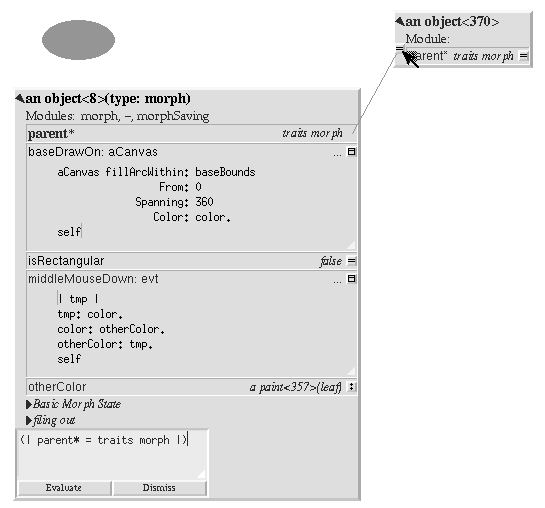
\includegraphics{Figure5.png}
\caption{Figure 5: A new traits object has been created to hold behavior to be shared by all instances of the morph. Arrow dragging is being used to make the parent slot of the new morph point to the new traits object.}\end{flushleft}\end{figure}

Now, the behavior to be shared can be moved from the prototype into the new traits object. Invoke the ``Move'' command on the middle-button menu for the \textbf{isRectangular} slot. This causes the slot to be plucked out of the object. Drop the slot onto the shared traits object. This causes it to be added to the that object. Repeat this process for the \textbf{baseDrawOn:} and \textbf{middleMouseDown:} slots.

The Self language uses slot inheritance to share both data (\textbf{isRectangular}) and behavior (\textbf{baseDrawOn:} and \textbf{middleMouseDown:}). The programming environment supports a similar kind of uniformity by allowing any slot to be moved or copied by via drag-and-drop. A entire category can also be copied or moved by dragging.

Note that when moving a slot between an object and its parent there is an interval during which the slot is not in either object. If a message matching the slot name is sent to the object during this interval, the object's response is be determined by a slot inherited from a parent higher in the inheritance chain, if any. If it is important to avoid this transient state, one can move the each slot by first copying it from the prototype into the parent and then remove it from the prototype. A slot is removed simply by moving it and dropping it onto the trash can morph (or by dropping it on the background and then dismissing it).
\begin{figure}[htbp]\begin{flushleft}
\capstart

\includegraphics{Figure6.png}
\caption{Figure 6: Using slot-dragging to move a slot into the new traits object. Using direct manipulation to move and copy slots makes programming feel like manipulating concrete objects. This narrows the gap between composition of graphical objects (building and modifying composite morphs) and programming.}\end{flushleft}\end{figure}

Now, changing the traits object changes the behavior of all instances. For example, the draw method in the traits can be changed to draw an unfilled oval. To demonstrate the power of shared behavior, first make several copies of the protypical oval using the ``Duplicate'' command on its right-mouse menu. Then modify the baseDrawOn: method in the shared traits as follows (note the change from ``fillArcWithin:'' to just ``arcWithin:''):
\begin{quote}

\begin{Verbatim}[commandchars=\\\{\}]
baseDrawOn: aCanvas = (
        aCanvas arcWithin: (baseBounds indent: 3)
                From: 0
                Spanning: 360
                Width: 3
                Color: color.
        self)
\end{Verbatim}
\end{quote}

The oval is drawn with a pen three-pixels wide. To accommodate the extra width, the rectangle passed to the canvas is indented by three pixels. Note: A morph should never draw outside its baseBounds. When this method is accepted, all copies of the prototype reflect the change. However, Morphic doesn't automatically redraw instances when the draw method is changed. To see the change, drag some large object over the ovals to make them redraw.
\begin{figure}[htbp]\begin{flushleft}
\capstart

\includegraphics{Figure7.png}
\caption{Figure 7: Changing the shared traits object changes the behavior of copies of the prototype (instances). In this case, the draw method has been changed to draw unfilled ovals.}\end{flushleft}\end{figure}

At this point, the prototype for a new kind of morph has been created and the behavior common to all its instances has been factored into a separate traits object to facilitate later changes. The next step is to install the prototype and its traits in the global and traits namespace objects. Doing this allows the morph prototype and its traits to be referred to by name.

First, summon outliners for the globals and traits namespace objects by evaluating the expressions ``globals'' and ``traits'' in any text editor. (That is, type the expression, select it, and invoke the ``Get Expression'' command in the middle-button menu of the editor.) Then, open an appropriate category for the new morph or create a new category. Within the chosen category of ``globals,'' create a slot to hold the new morph's prototype by invoking the ``Add Slot'' command and accepting the following expression:
\begin{quote}

\begin{Verbatim}[commandchars=\\\{\}]
\PYG{n}{ovalMorph} \PYG{o}{=} \PYG{n}{nil}
\end{Verbatim}
\end{quote}

Next, invoke the ``Grab pointer'' command by pressing the middle-button menu on the button on the right side of the new ovalMorph slot. Drop the end of the pointer over the new morph prototype and release the mouse. This makes the new slot point to the new morph prototype. Repeat the procedure just described to create an ``ovalMorph'' slot in the traits namespace and point it to the traits object for the new morph.
\begin{figure}[htbp]\begin{flushleft}
\capstart

\includegraphics{Figure8.png}
\caption{Figure 8: Installing the new morph prototype and traits object in the globals and traits namespace objects. In each case, a new constant slot is created in the appropriate category, then arrow-dragging is used to make the new slot point to the desired object.}\end{flushleft}\end{figure}

Finally, invoke the ``Make creator'' middle-button menu command on each new ``ovalMorph'' slot to designate it as that morph's creator. This informs the system that the given slot is the given object's home in the global namespace. (An object may be reachable via several global slots; setting its creator path distinguishes one of these slots as the object's official ``home address.'' This information is used to determine the object's name, as well as which the module in which to record information about the object as a whole, such as the object comment.) In a few seconds (if outliner updating is on), the outliner titles of the ovalMorph prototype and its traits object will be updated to show the new names for these objects.

To allow a composite morph containing ovalMorphs to be saved in a file, the prototype method in the prototype (not the traits!) must return the prototype ovalMorph. The ovalMorph prototype already has a prototype method that was copied from the original morph prototype. Change the body of the prototype method in the ``filing out'' category to:
\begin{quote}

\begin{Verbatim}[commandchars=\\\{\}]
\PYG{n}{ovalMorph}
\end{Verbatim}
\end{quote}
\begin{figure}[htbp]\begin{flushleft}
\capstart

\includegraphics{Figure9.png}
\caption{Figure 9: Setting the creator slot of the new traits object. The system uses this information to name objects, among other things. Note that the title of the prototype (on the left) has already been updated to reflect its new name.}\end{flushleft}\end{figure}

Many Smalltalk programming environments allow an instance variable to be added to a class at runtime. The new instance variable is propagated down to all subclasses and added to all existing instances of the class and its subclasses with an initial value of nil. The Morphic programming environment can provide a similar service for the copied-down slots of prototypes, with two significant differences: (1) changes to the values of a copied down slots are propagated, as well as slot additions and removals and (2) changes are propagated only to objects registered in the global namespace (other prototypes), not to clones of those objects (instances).

The system can be told to maintain the copied-down slots of the ovalMorph prototype automatically by setting its copy-down parent (Figure 10). Select the ``Show Annotation'' command in the middle-button menu on the title of the ovalMorph's outliner. Set the copy-down parent field to ``morph'', the copy-down selector to ``copyRemoveAllMorphs'', and press the green (top) button to accept this change. (The copy-down selector is sent to the copy-down parent to create a fresh copy from which to copy slots.) The system will ask if the slots ``parent'' and ``prototype'' should be omitted from the copy-down operation, since their contents differ from that of that of the copy-down parent. They should be.

Finally, it would be nice to be able to save the prototype and traits for the new ovalMorph in a file so that it can be archived or read into another Self world. Several steps are required. First, the module itself must be created. The system will create a new module (after getting confirmation from the user) the first time its name is used. Then, the slots in the globals and traits namespace object must be assigned to the new module. Finally, the non-copied-down slots in the prototype and traits objects are assigned to the module. This may sound tedious, but the system provide several shortcuts to accelerate the process.

To set the module for the new morphs home slot, invoke ``Show annotation'' on the ovalMorph slot in the globals object, type ``ovalMorph'' in the module field, and accept the change (Figure 11). Since this is a new module, the system will ask whether a new module should be created (yes), whether it should be a submodule of an existing module (no), and what subdirectory it should be stored into (``applications''). Set the module of the ovalMorph slot in the traits object the same way.
\begin{figure}[htbp]\begin{flushleft}
\capstart

\includegraphics{Figure10.png}
\caption{Figure 10: Setting the copydown parent for the new prototype.}\end{flushleft}\end{figure}
\begin{figure}[htbp]\begin{flushleft}
\capstart

\includegraphics{Figure11.png}
\caption{Figure 11: Setting the modules for the namespace slots. The module will be created if it doesn't already exist; the system asks the user several questions about where the new module should live and whether it is a submodule of some existing module.}\end{flushleft}\end{figure}

All the slots in an object (or within one category of that object) can be assigned to a module in a single operation. To assign the slots of the new traits object to the new module, invoke the ``Set module...'' command on the header of its outliner. The system will ask which slots should be assigned to the module (all) and which module to put them into (ovalModule). After a few seconds, the module summary at the top of the outliner should update to indicate that all slots of the traits object are in ovalModule. Repeat this procedure to assign all the slots of the ovalMorph prototype to ovalModule.
\begin{figure}[htbp]\begin{flushleft}
\capstart

\includegraphics{Figure12.png}
\caption{Figure 12: Assigning all the slots of the new traits object to the new module.}\end{flushleft}\end{figure}

Now that all the slots of the new morph and its prototype have been assigned to the new module, the module can be filed out. Invoke the ``Changed modules...'' command on the background menu to get the changed modules morph. Then press the little button marked ``w'' to the right of ``ovalModule''. The system will save the code for the module in a file named ``ovalModule'' in the ``applications'' subdirectory of the current working directory. (If this directory doesn't exist, the system will complain. Create the directory and try the fileout operation again.) The oval morphs module can later be loaded into a snapshot by evaluating the expression:
\begin{quote}

\begin{Verbatim}[commandchars=\\\{\}]
bootstrap read: 'ovalModule' From: 'applications'
\end{Verbatim}
\end{quote}
\begin{figure}[htbp]\begin{flushleft}
\capstart

\includegraphics{Figure13.png}
\caption{Figure 13: Saving the code for the new morph in a module file.}\end{flushleft}\end{figure}


\subsection{Morph Creation: The Top-down Approach}
\label{morphic:morph-creation-the-top-down-approach}
The top down approach to creating a new morph is similar to the approach just described, except that one plans to make a first-class citizen from the beginning. Thus, the order of steps is slightly different. Here is a brief outline of the procedure:
\begin{enumerate}
\item {} 
Add a slot to the traits namespace object (using ``Add Slot''):
\begin{quote}

\begin{Verbatim}[commandchars=\\\{\}]
ovalMorph = (\textbar{} parent* = traits morph \textbar{})
\end{Verbatim}
\end{quote}

\item {} 
Add a slot to the globals namespace object:
\begin{quote}

\begin{Verbatim}[commandchars=\\\{\}]
ovalMorph = (\textbar{} parent* = traits ovalMorph \textbar{})
\end{Verbatim}
\end{quote}

\item {} 
Make each new slot be the creator of its contents (using ``Make creator'').

\item {} 
Set the copy-down parent of the prototype to morph (via ``Show annotation'' on its outliner).

\item {} 
Set the module of the two namespace slots to ovalModule (creating the new module in the process).

\item {} 
Assign all slots of the new traits and prototype objects to ovalModule.

\item {} 
Start programming the new behavior.

\end{enumerate}

This procedure does all the housekeeping chores up front, so the module can be filed out at any time. As the programmer works, the system will deduce that any slots added to ovalMorph's traits or prototype should be placed in the same module as the other slots in that object (ovalModule). In a future release of the system, the initial housekeeping may be automated. This would make creating a new kind of morph a one-step operation.


\section{Saving a Composite Morph}
\label{morphic:saving-a-composite-morph}
The system includes an experimental facility for store the structure of a composite morph to a file. This allows a morph constructed by direct manipulation to be saved into a file that can be read later to reconstruct the morph. This is how the ``factory'' was created. The morph saving facility requires that every morph and submorph to be saved supply implementations of the messages \textbf{slotsToNotFileOut}, \textbf{appendOtherSlotsOnto:}, \textbf{storeStringNeeds}, and \textbf{prototype}. Unfortunately, because morph saving was added later as an experiment, not all morphs have been retro-fitted with implementations of these messages. The enterprising user could easily infer how to add the required support to morphs that do not yet have it.

Suppose one has created a column of useful buttons that one wishes to save. (Fortunately, buttons, columns, rows, frames, and labels are among the morphs that do support saving.) To save this morph, create an outliner for it and then evaluate in that outliner:
\begin{quote}

\begin{Verbatim}[commandchars=\\\{\}]
\PYG{n}{saveMorphInFile}
\end{Verbatim}
\end{quote}

The system will prompt for a file name and will give graphical feedback as each component morph is stored. The file can later be read by evaluating:
\begin{quote}

\begin{Verbatim}[commandchars=\\\{\}]
worldMorph loadMorphFromFile
\end{Verbatim}
\end{quote}

Again, the system will prompt for the file name. A copy of the morph that was saved will be added to the hand. The return value of the expression will also be added to the hand, which may temporarily hide the new morph. Click any mouse button to put down the two objects, then move the top one out of the way.


\section{Handling User Input}
\label{morphic:handling-user-input}

\subsection{Handling Events}
\label{morphic:handling-events}
Morphic represents user actions such as pressing a key or mouse button using \textbf{ui2Event} objects. A \textbf{ui2Event} actually carries two kinds of information: its \emph{type}, such as ``leftMouseDown'', and the state of the mouse buttons and certain keyboard keys when the event occurred. This allows a program to tell, for example, if the shift key was held down when the left mouse button was pressed. As events occur, they are placed into a buffer. Morphic removes and processes events from this buffer in order. Thus, even if a user occasionally gets ahead of the system, the system will eventually catch up.

A morph can handle a given kind of event simply by implementing one of the following messages:
\begin{quote}

\begin{Verbatim}[commandchars=\\\{\}]
keyDown: evt
keyUp: evt
mouseMove: evt
leftMouseDown: evt
leftDoubleClick: evt
leftMouseUp: evt
middleMouseDown: evt
middleDoubleClick: evt
middleMouseUp: evt
rightMouseDown: evt
rightDoubleClick: evt
rightMouseUp: evt
\end{Verbatim}
\end{quote}

The event is always supplied so that its state can be examined. The default behavior of the \textbf{leftMouseDown:} message is to pick up the composite morph containing the morph that gets the event. (That is, the left mouse button generally means ``move''.) The default behavior of the \textbf{rightMouseDown:} message is to pop up the morph menu (the ``blue'' menu). The default behavior of the other messages is to return the special \textbf{dropThroughMarker} object, indicating that the event is not processed by this morph.

Submorphs of a morph are displayed in front of their owning morph. By default, submorphs are usually given the first opportunity to handle incoming events. If a submorph does not handle an event, it returns the \textbf{dropThroughMarker} object, and Morphic gives the submorph behind it a chance to handle the event. Each user generates events at the current location of their cursor. One can visualize an event as ``falling down through'' the submorphs of the composite morph at that location until either the event lands on a submorph that handles it or until all the submorphs of the composite at that point are exhausted. However, events do not fall between top-level morphs. For example, if an outliner is covered by a morph that does not handle middleMouseDown events, one cannot invoke the middle button menu of the outliner through the intervening morph.

In some cases, a morph may wish to handle certain events before its submorphs. For example, a ui2Menu morph handles leftMouseDown events itself rather than letting its component buttons get them in order to highlight the button under the cursor and to pop down the menu when a selection is made. A morph can arrange to handle certain kinds of events before its submorphs by overriding the \textbf{allowSubmorphsToGetEvent:} message.

There are actually two classes of events. KeyDown events, the three mouseDown events, and the three doubleClick events are dispatched using the ``falling through the submorphs'' technique just described. The other events—keyUp, mouseMove, and the three mouseUp events are dispatched only to interested \emph{subscribers}. The rationale is that some morphs are interested in discrete events, such as mouseDown transitions, while others need to track the mouse or keyboard over an extended period of time. Dispatching high-frequency events such as mouseMove to uninterested morphs would be inefficient. Futhermore, some morphs need to get events even when the cursor is no longer over the morph. For example, a click-to-type editor should continue to get keyDown events until another editor is clicked. In short, Morphic supports both spatial and subscription-based event dispatching because both are useful.

The events generated by a particular user are dispatched from the handMorph associated with that user. Each hand-Morph keeps a list of subscribers interested in various kinds of events. A morph asks the appropriate handMorph to start or stop its subscription to a particular kind of event. Every event has a reference to the hand that generated that even. Thus, a morph that wishes to track the mouse until the button is released (e.g., sliderMorph) would do the following:
\begin{enumerate}
\item {} 
on leftMouseDown, execute ``evt sourceHand subscribeUntilAllUp: self''

\item {} 
on mouseMove, update the slider position from the current mouse position (which is in global coordinates)

\end{enumerate}


\subsection{Mapping special characters to actions}
\label{morphic:mapping-special-characters-to-actions}
When a morph receives the keyDown: message, the next step is the interpretation of any control-, meta- or command- keystrokes. For example, on the Macintosh, a command-X should perform a cut operation. A morph wishing to respect these conventions should do two things: it should inherit from \code{traits ui2Event ignoreSpecialCharactersMixin}, and it should, upon receiving the keyDown: message, send \code{sendMessageToHandleKeyboardEventTo:} the event, passing itself as the argument. The latter message tells the event to decode any special characters and send an apprpropriate message back to its argument. The mixin provides default behavior.


\section{Drag and Drop}
\label{morphic:drag-and-drop}
A morph can perform some action when another morph is dropped onto it and can decide which dropped morphs it will accept. In addition, the dropped morph can perform some action in response to being dropped.

To accept dropped morphs, a morph must respond affirmatively to the message:
\begin{quote}

\begin{Verbatim}[commandchars=\\\{\}]
wantsMorph: m Event: evt
\end{Verbatim}
\end{quote}

The morph to be dropped is supplied as an argument to allow the receiving morph to decide if it wishes to accept the drop. For example, a printer icon morph might accept only document morphs. If the target morph agrees to accept the dropped morph, the target is then sent the message:
\begin{quote}

\begin{Verbatim}[commandchars=\\\{\}]
addDroppingMorph: m Event: evt
\end{Verbatim}
\end{quote}

to actually perform the drop action. Part of this action should be to put the dropping morph somewhere or delete it. For example, the printer icon morph might queue a print request, then add the document morph to a folder morph representing the printed documents.

Finally, the dropped morph is informed of the drop (post facto) by sending it the message:
\begin{quote}

\begin{Verbatim}[commandchars=\\\{\}]
justDroppedInto: m Event: evt
\end{Verbatim}
\end{quote}

The event is provided in these messages to allow the morph to examine the state of the mouse buttons or modifier keys at the time of the drop.


\section{Automatic Layout}
\label{morphic:automatic-layout}

\subsection{Packing}
\label{morphic:packing}
Automatic layout relieves the programmer from much of the burden of laying out the components of a composite morph such as a dialog box. By allowing morphic to handle the details of placing and resizing the components, the programmer can focus on the \emph{topology} of the layout, without worrying about the exact positions and sizes. Automatic layout also allows composite morphs to adapt gracefully to size changes, including font size changes.

\emph{Layout morphs} manage the placement and sizing of their submorphs. Layout morphs currently include rowMorphs, columnMorphs, frameMorphs and their descendents. All other morphs leave the size and placement of their submorphs alone. The current set of layout morphs all use the same layout strategy: linear, non-overlapping packing. Rows pack horizontally from left-to-right. Columns, frames, and their descendents pack vertically from top-to-bottom. This simple approach, while it does not handle every conceivable layout problem (e.g., tables whose rows and columns adjust to the size of their contents), is surprisingly powerful. All automatic layout in morphic is based on nested combinations of rows and columns.

Linear packing is best explained procedurally. Consider a rowMorph. Its task is to arrange its submorphs into a row such that the left edge of each morph just touches the right edge of the next morph. The submorphs are processed in order; that is, the first submorph will be placed at the left end of the row, then the next submorph will be placed to the right of the first, and so on. The last submorph will be placed at right-most end of the row. Notice that the order of the submorphs is not affected by the packing process. Also notice that the packing is done only in one primary dimension—the horizontal dimension in this case. The other dimension is also considered during packing, and is controlled by the \emph{justification} parameter of the row. Depending on this parameter, the tops, bottoms, or centers of the submorphs can be aligned with the top, bottom, or center of the row.


\subsection{Space-filling}
\label{morphic:space-filling}
For simplicity, the packing strategy was described as if the submorphs to be packed were all rigid. In order to support ``stretchy'' layouts, morphs can be designated as \emph{space-filling}. (Note: The source code uses the older term, \emph{flexible}.) When there is extra space, a space-filling morph expands to fill this space. If there is no extra space, a space-filling morph shrinks to its minimum size. When there are several space-filling morphs in a single row or column, any extra space is divided evenly among them.

Space-filling morphs can be used to control the placement of submorphs within the primary dimension when a row or column is stretched. For example, suppose one wanted a row with three buttons, one at the left end, one at the right end, and one in the middle. This can be accomplished by inserting space-filling morphs between the buttons:
\begin{quote}

\begin{Verbatim}[commandchars=\\\{\}]
\textless{}button1\textgreater{}\textless{}spacer\textgreater{}\textless{}button2\textgreater{}\textless{}spacer\textgreater{}\textless{}button3\textgreater{}
\end{Verbatim}
\end{quote}

When the row is stretched, the extra space is divided evenly between the two spacers, button2 stays in the center, and button3 stays at the far right. By making the color of the spacers match that of the underlying row, they become effectively invisible. This is a common technique.
\begin{figure}[htbp]\begin{flushleft}
\capstart

\includegraphics{Figure14.png}
\caption{Figure 14: Using flexible spacer morphs to space buttons evenly within a row. Normally these spacers would be made the same color as the row, making them effectively invisible}\end{flushleft}\end{figure}


\subsection{Shrink-Wrapping}
\label{morphic:shrink-wrapping}
It is sometimes desirable for the size of a morph to depend on the sizes of its submorphs. For example, the size of a button should depend on the size of its label. (It would be annoying if it didn't; the programmer would have to manually resize the button after changing the label.) A morph designated as \emph{shrink-wrap} shrinks (or grows) to the smallest size that accommodates the size requirements of its submorphs.


\subsection{Minimum Sizes}
\label{morphic:minimum-sizes}
Morphs have a minimum size in each dimension (\textbf{minWidth} and \textbf{minHeight}). These sizes determine the minimum amount of space that will be allocated to a morph during layout. The minimum size of a morph takes into account the minimum sizes of its submorphs. For example, the minimum width of a row is the sum of the minimum widths of its submorphs (plus a little bit for a border, if it has one).

The absolute minimum width and height of a morph, even when it has no submorphs, is specified by its \textbf{baseMinWidth} and \textbf{baseMinHeight}. For some kinds of morph, these values are stored in assignable slots in the morph. For others, these values are defined by inherited constant slots to save space. One can use these attributes to give a space-filling morph a minimum size.


\subsection{Resize Attribute Summary}
\label{morphic:resize-attribute-summary}
The resizing behavior of a morph in one dimension is completely independent of its behavior in the other dimension; that is, a morph actually has two independent resizing attributes, one for the horizontal dimension and one for the vertical dimension.

To summarize, the resizing behavior of a morph along a given dimension is controlled by its resizing attribute, which has one of three values:
\begin{quote}

\textbf{rigid} The morph is not resized.

\textbf{space-filling} In a row or column, the size of the morph adapts to fill the available space. Extra space is shared evenly with any other space-filling morphs in that row or column.

\textbf{shrink-wrap} The morph is shrunk to just fit around its submorphs, or to its minimum size, whichever is smaller. Enclosed space-filling morphs are shrunk if necessary.
\end{quote}

A morph's minimum size in a given dimension determines the smallest amount of space that should be allocated to it during layout. The core sampler and/or properties sheet can be used to change these attributes.


\section{Animation}
\label{morphic:animation}
Animation can be used to make an interactive application seem more alive and can convey valuable information. However, animation can become annoying if the user has to wait until the animation completes before doing anything else. In Morphic, animation and user actions are concurrent, and multiple animations can be active while multiple users interact with the system.
\begin{figure}[htbp]\begin{flushleft}
\capstart

\includegraphics{Figure15.png}
\caption{Figure 15: Three simultaneously active morphs: an ideal gas simulation, a digital clock, and an outliner on the Self object underlying one of the atoms in the simulation. The clock updates every second, the simulation runs continuously, and the outliner periodically updates its center and velocity slot values as the underlying atom moves. A morph continues to operate while it is being moved (the clock is being moved here) or while an external animation is applied to it. Note that multiple users can be active simultaneously; this example shows the cursors of two users.}\end{flushleft}\end{figure}

There are two ways to achieve animation. First, a morph can have lightweight autonomous behavior which typically, although not necessarily, appears as animation. For example, a clock might advance the time or a discrete simulation might compute simulation steps. Second, Morphic includes a kit of external animation behaviors that can be applied to any morph, including motion, scaling, and color change animations.

Although autonomous behavior and external animations are implemented using the same underlying mechanism, they have different purposes and are specified in different ways. The autonomous behavior of a morph is an intrinsic property of that morph. For example, updating the time is central to being a clock morph. Autonomous behavior is defined in the morph itself. External animation behaviors, on the other hand, are typically transient and imposed from outside. For example, the Self programming environment gives feedback for certain actions by ``wiggling'' the relevant morph. An external animation is specified by creating a separate animation activity object and applying it to the morph to be animated. Animation is orthogonal to autonomous behavior; for example, a clock morph would continue to run even while a motion animation whisked it across the screen.


\subsection{Stepping}
\label{morphic:stepping}
The autonomous behavior of a morph is defined by its \emph{step} method. For example, to make a simple digital clock, one could add the following slot to a copy of labelMorph:
\begin{quote}

\begin{Verbatim}[commandchars=\\\{\}]
step = ( label: time current timeString )
\end{Verbatim}
\end{quote}

The clock is activated by asking the system to send the ``step'' message to it either continuously (every display update cycle) or at periodic intervals (e.g., once per second). Make sure the labelMorph is visible in the world (use the ``Show Morph'' menu command if necessary), then, in an evaluator on its outliner, evaluate:
\begin{quote}

\begin{Verbatim}[commandchars=\\\{\}]
getSteppedEveryMSecs: 1000
\end{Verbatim}
\end{quote}

This will cause the \textbf{step} message to be sent to the morph once per second (i.e., every 1000 milliseconds), causing it to display a formatted string representing the current time. Step messages are sent synchronously during the display update cycle. This has the advantage of simplifying synchronization but requires that step methods complete quickly to avoid delaying user interactions.

The message \textbf{stopGettingStepped} can be sent to the morph to turn off stepping for that morph. Morphic automatically stops stepping when the target morph is removed from the world. To make the clock morph reactivate itself when dropped back into the world, add the following slot:
\begin{quote}

\begin{Verbatim}[commandchars=\\\{\}]
justDroppedInto: m Event: evt = (
        isInWorld ifTrue: [ getSteppedEveryMSecs: 1000 ]).
\end{Verbatim}
\end{quote}


\subsection{External Animation}
\label{morphic:external-animation}
External animation of a morph is achieved by scheduling an \emph{animation activity} with that morph as its target. An animation activity changes some property of its target gradually over the course of a number of display cycles (frames). For example, a \textbf{positionAnimator} animates a change in its target morph's location. The programmer specifies the initial and final values of the property to be changed (e.g., the starting and ending position) and the duration over which the change should occur. The duration can be defined in two ways. \emph{Frame-based} animation lets the programmer control animation smoothness by specifying that the animation should take a given number of frames regardless of the time per frame. \emph{Time-based} animation lets the programmer specify the desired amount of time the animation should take, but the number of intermediate frames depends on the time per frame, which may vary with system load, scene complexity, and other factors. Animations can be paced linearly or slow-in-slow-out. A slow-in-slow-out animation starts slowly, builds to a maximum pace, then decelerates. There are activities that animate the position, size, and color of morphs, activities that send arbitrary messages, and compound activities that combine a set of other activities either sequentially or concurrently. In fact, this activity architecture is the basis of all animation in Morphic: an activity called a \textbf{periodicStepActivity} is used to implement the stepping facility.


\section{Other Issues}
\label{morphic:other-issues}

\subsection{Local versus Global Coordinates}
\label{morphic:local-versus-global-coordinates}
The position of a morph is defined relative to the position of its owner. This makes it unnecessary to update the positions of all the submorphs when moving a composite morph. However, it also means that morphs with different owners have positions in different coordinate systems. In order to compare the positions of morphs having different owners, it is necessary to use their positions in the world's coordinate system, which are computed by sending the \textbf{globalPosition} message to each morph.


\subsection{Synchronization}
\label{morphic:synchronization}
Animation, stepping, and other activities are handled synchronously, as part of the basic user interface loop. Thus, a sequence of actions done by an activity or a \textbf{step} method appear to happen atomically; the user never sees the morph in an intermediate state in which some but not all of the actions have taken place. For example, if a morph is removed from one morph and added to another, the user never sees the transient state in which the morph is not in the world at all. Likewise, any layout modifications resulting from user actions—such as adding a new morph to a row—appear to happen atomically; one never sees a partially complete layout.

Often, however, an independent Self thread wishes to manipulate morphs in the user interface. In order to make such actions appear atomic, they should be done under the protection of the UI synchronization semaphore. The preferred way to do this is to wrap the action or actions in a block to be executed between display cycles of the morph's world:
\begin{quote}

\begin{Verbatim}[commandchars=\\\{\}]
aMorph safelyDo: [ ... ]
\end{Verbatim}
\end{quote}

Synchronization errors usually appear as intermittent graphical glitches, although in rare cases the submorph structure may be corrupted (e.g., a morph appearing in the submorph lists of multiple morphs).


\subsection{Display Updating}
\label{morphic:display-updating}
Morphic uses a double-buffered, incremental algorithm to keep the screen updated. This algorithm is efficient (it tries to do as little work as possible to update the screen after a change) and high-quality (the user does not see the screen being repainted). It is also mostly automatic; many applications can be built without the programmer ever being aware of how the display is maintained. The description here is mostly for the benefit of those curious about how the system works.

Each morphic screen window displays the contents of some worldMorph. A worldMorph keeps a list of rectangular ``damaged'' regions of the screen. Every morph can compute a rectangle that encloses its entire visible representation. When a morph changes its appearance (for example, its color), it sends itself the \textbf{message} changed. This causes its bounding rectangle to be translated into global coordinates and added to the damage list of the worldMorph that contains it. (This worldMorph is found by starting at the morph and following the \textbf{owner} chain; the worldMorph is the last morph in this chain.) On the next display update cycle, the worldMorph redraws the portions of all morphs that intersect rectangles in the damage list (via an off-screen buffer), including the morph that was changed. The world-Morph then clears its damage list to prepare for future damage reports.

When a morph changes size or position, damage is reported both before and after the change. This causes the screen to be updated at both the old and new size or position.

Typically, the implementor of a morph writes code to send the changed message automatically after updating any slot that affects the morph's appearance. For example, the \textbf{color:} message defined in traits morph sends changed automatically. Likewise, external animation activities report appropriate changes. Thus, the client of a morph usually need not send \textbf{changed} explicitly.


\subsection{Layout Updating}
\label{morphic:layout-updating}
Morphic also maintains morph layout incrementally. When a morph is changed in a way that could influence layout (e.g., when a new submorph is added to it), the message \textbf{layoutChanged} is sent to the morph. This triggers a chain of activity. First, the layout of the changed morph is updated. This may change the amount of space apportioned to some of its submorphs, causing their layouts to be updated. Then, if the space requirements of the changed morph have changed (e.g., if it needs more space to accommodate the newly added submorph), the layout of its owner is updated, and possibly its owner's owner, and so on. In some cases, the layout of every submorph in a deeply-nested composite morph may need to be updated. Fortunately, there are many cases where the layout updates can be localized. Morphic detects these cases, thus saving a great deal of unnecessary work.

As with \textbf{changed} messages, morph clients usually need not send \textbf{layoutChanged} explicitly since the most common operations that affect the layout of a morph—such as adding and removing submorphs or changing its size—take care of this already.

Normally, layout is performed incrementally after every morph add or remove operation. However, when a large composite morph is to be constructed, the cost of the repeated layout operations can be significant. The programmer can ameliorate this problem by using the batch operation \textbf{addAllMorphs:} rather than a sequence of individual \textbf{addMorph:} operations.

If a morph is not in a worldMorph, however, all layout is deferred. This is done partly to optimize creating large composite morphs (which are often constructed ``off-line'' and then added to the world) and partly because the exact size of labelMorphs depends on font metrics that may vary from one X server to another. Thus, the layout of a morph containing labels would have to be recomputed in the context of a particular world anyway. Occasionally, one needs to know the exact size of a newly created morph (for example, to ensure that a menu does not pop up partially off the edge of the screen). In such cases it may be necessary to temporarily add the morph to the world in some remote location (such as -1000000 @ -1000000) to force it to be laid out.


\subsection{Morph Copying}
\label{morphic:morph-copying}
When a composite morph is copied, its entire submorph tree is traversed and copied to produce a duplicate with the same structure. However, simply copying the structure is not quite enough because some of the morphs within a composite morph may refer to other morphs within the composite. For example, the buttons of a radarView refer to the radarDisplay morph. When a radarView morph is copied, the buttons of the copy must be updated to point to the radarDisplay morph in the copy, not that in the original radarView. A simplified diagram of this process is shown in Figure 16.

Sometimes a morph may need to do something special when it is copied. In this case, the message \textbf{baseCopy} should be overridden rather than \textbf{copy}. See \textbf{traits ui2Button} for an example of how this is done.
\begin{figure}[htbp]\begin{flushleft}
\capstart

\includegraphics{Figure16.png}
\caption{Figure 16: Copying a composite morph. First, the submorph structure of the original morph is copied (a). Then, references among the submorphs of the composite updated to mirror those of the original (b).}\end{flushleft}\end{figure}


\section{Morph Responsibilities}
\label{morphic:morph-responsibilities}
There are two messages that each type of morph is expected to implement: \textbf{morphTypeName} and \textbf{prototype}. The first returns a string used to show the type of a morph in the user interface (e.g., in the core sampler) while the second, which should return the prototype for the morph, is used by the morph filing out code.

Two other messages may need to be overridden. These are:
\begin{quote}

\textbf{isRectangular} This message is used to optimize the drawing of shadows for morphs whose display completely fills their bounding rectangle. The default implementation returns \textbf{true}, so non-rectangular morphs such as circleMorphs must provide an implementation that returns \textbf{false}. (Hint: If a non-rectangular morph casts a rectangular shadow, someone probably forgot to override this message.)

\textbf{mapReferencesUsing}: This message is sent during copying to update any references between the submorphs of a composite morph. Its argument is a dictionary mapping submorphs in the old composite morph to the corresponding submorphs in the copy. Morphs whose slots may contain references to other morphs within a composite should override this message to update these slots during copying. For example, a ui2ButtonMorph overrides this message in order to update its “target” slot. That way, if the button and its target are both embedded in some composite morph that is copied, the button in the copy will refer to the target in the copy. See \textbf{traits colorChangerMorph} for an example.
\end{quote}


\section{Some Useful Morphs}
\label{morphic:some-useful-morphs}
The Self system comes with a large library of morphs. While some morphs exist solely to supporting the programming environment, many are general-purpose and can be reused to construct new applications. This section mentions some of the most useful and reusable morphs. To find out more about a given morph, use the programming environment to examine its prototype and traits objects. Useful comments are sometimes buried in the bodies of methods.

\emph{Widget morphs} are interactive, allowing the user to invoke an action or input some data.
\begin{quote}

\textbf{sliderMorph} Allows the user to specify a numerical value in some range. When the slider is manipulated, its target object is sent a user-specified message with the new slider value as an argument.

\textbf{ui2Button} Executes a user-specified script when the button is pressed. The script can refer to the button's target. The target of a button or slider morph can be set by using the middle-mouse menu “Set Target” command. This sets the target slot of the button or slider to the morph directly below it. Buttons are often decorated with a textual label, but a button can contain arbitrary morphs instead of, or in addition to, this label.

\textbf{ui2Menu} A column full of buttons. A menu can be “pinned down” using the unlabeled button at its top. It can then be manipulated or disassembled like any other morph. Menus support a rich set of messages for adding normal or grayed out buttons and for inserting dividing lines.
\end{quote}

\emph{Structural morphs} are typically used to bind morphs together and arrange them into a pleasing layout.
\begin{quote}

\textbf{rowMorph and columnMorph}  Pack their submorphs into a row or column. These morphs offer several justification options and can also provide a border of empty space around their contents.

\textbf{frameMorph}  Like a columnMorph, except that it can display various kinds of borders around its contents. Bezeled frameMorphs are used heavily in the programming environment to provide a three-dimensional look.

\textbf{spacerMorph} While many types of morph (such as an empty rowMorph) could be used to fill a space between morphs, it is preferable to use a \textbf{spacerMorph} to make it clear that the only purpose of the morph is to control spacing. (Morphic allows users to customize the user interface by directly manipulating morphs. Thus, just as is it important to write readable programs, it is important to build composite morphs with “readable structure.”) Often, a spacerMorph is used to provide a fixed amount of space between submorphs in a rowMorph (or columnMorph). To accomplish this, the spacerMorph should be of the desired width, be rigid horizontally and space-filling vertically, and be the same color as the rowMorph. The message \textbf{copyH:Color:} (or \textbf{copyV:Color:} to creating a vertical spacer for use in a column) can be sent to spacerMorph to create a new spacerMorph with these properties. The other common use of spacerMorphs is to provide a stretchy space between morphs; the expression “spacerMorph copy beFlexible” makes a spacerMorph that does the job. Setting the \textbf{baseMinWidth:} or \textbf{baseMinHeight:} of such a spacer ensures that at least the given amount of space will be provided.
\end{quote}

Other morphs supply decorative or information content for user interfaces.
\begin{quote}

\textbf{labelMorph} displays a single-line string in a single font style, size, and color.

\textbf{circleMorph} displays a filled circle.

\textbf{pixmapMorph} displays an image (currently, at most 8 bits deep).

\textbf{movieMorph} cycles through a sequence of images as it is stepped.
\end{quote}

The library includes two kinds of text editors.
\begin{quote}

\textbf{editorMorph} a general editor that allows arbitrary morphs to be embedding in the text.

\textbf{uglyTextEditor} a simple, text-only editor that is a bit faster for editing larger amounts of text.
\end{quote}

Many applications implement specialized content morphs. For example, the Self programming environment defines morphs that represent Self objects, slots, and categories.


\section{The Graphical Environment}
\label{morphic:the-graphical-environment}
Morphic hides many details of the underlying graphics system. This both simplifies programming and provides portability: the layer of abstraction between the programmer and the underlying graphics system allows the implementation of the low-level graphics to be changed without affecting programs written by clients. While the current version of the system is built on the X window system, it could be ported to other window systems fairly easily (although the target window system should support color or grayscale for good results). One might even create a Postscript implementation of the morphic graphics interface to allow morphs to render themselves on paper.

The graphics interface is implemented by canvas objects. There may eventually be many kinds of canvases for rendering onto displays of differing resolutions, color properties, or bit-depths. The current system provides four types of canvas. \textbf{WindowCanvas} and \textbf{pixmapCanvas} draw onto a window or an offscreen buffer via the X protocol. A \textbf{NullCanvas} has the same interface but does not actually draw anything; it can be used to factor out the cost of graphics during performance analysis. \textbf{ColorRecordingCanvas} is used internally by the colormap manager. All canvases implement the following messages for drawing geometric shapes:
\begin{quote}

draw a single pixel

\begin{Verbatim}[commandchars=\\\{\}]
point: p Color: c
\end{Verbatim}

outline or fill a rectangle or fill the entire canvas

\begin{Verbatim}[commandchars=\\\{\}]
rectangle: r Color: c
rectangle: r Width: w Color: c
fillRectangle: r Color: c
fillColor: c
\end{Verbatim}

draw a solid or dashed line or a connected sequence of line segments

\begin{Verbatim}[commandchars=\\\{\}]
line: pt1 To: pt2 Color: c
line: pt1 To: pt2 Width: w Color: c
dashedLine: pt1 To: pt2 DashSize: d Offset: o Color: c
dashedLine: pt1 To: pt2 Width: w DashSize: d Offset: o Color: c
lines: pointList Color: c
lines: pointList Width: w Color: c
\end{Verbatim}

outline or fill a polygon

\begin{Verbatim}[commandchars=\\\{\}]
polygon: pointList Color: c
polygon: pointList Width: w Color: c
fillPolygon: pointList Color: c
\end{Verbatim}

outline or fill a circle

\begin{Verbatim}[commandchars=\\\{\}]
circleCenteredAt: pt Diameter: d Color: c
circleCenteredAt: pt Diameter: d Width: w Color: c
fillCircleCenteredAt: pt Diameter: d Color: c
\end{Verbatim}

outline or fill a wedge cut by the given angles from an ellipse bounded by the given rectangle

\begin{Verbatim}[commandchars=\\\{\}]
arcWithin: r From: startAngle Spanning: spanAngle Color: c
arcWithin: r From: startAngle Spanning: spanAngle Width: w Color: c
fillArcWithin: r From: startAngle Spanning: spanAngle Color: c
\end{Verbatim}

draw a simple or compound curve

\begin{Verbatim}[commandchars=\\\{\}]
bezier: pt1 Control: c1 Control: c2 To: pt2 Width: w Color: c
bSpline: controlPoints Width: w Color: c
catmullRomSpline: controlPoints Width: w Color: c
\end{Verbatim}

draw text in the given font and size

\begin{Verbatim}[commandchars=\\\{\}]
text: s At: pt Font: fName Size: fSize Color: c
\end{Verbatim}

display a portable pixel-based image (a ui2Image)

\begin{Verbatim}[commandchars=\\\{\}]
image: i At: pt
\end{Verbatim}
\end{quote}

Canvases maintain an offset, allowing graphic operations to be automatically translated. (Canvases also maintain a scale factor, but scaling is not currently used and is probably buggy. Furthermore, image scaling is not implemented.)

In morphic, unlike many graphics packages, the graphics context is hidden from the programmer; all the common parameters that control the behavior of a given drawing command—such as color and line width—are passed as explicit parameters. A few infrequently changed parameters, such as the fill pattern and the clipping rectangle, can be changed temporarily via messages such as \textbf{withPattern:Do:} and \textbf{withClip:Do:}. The canvas handles these messages by changing the state of the underlying graphics context, executing the block provided (which presumably issues some drawing commands to that canvas), and restoring the original state of the graphics context. Nested invocations of withClip:Do: are handled sensibly: a stack of clipping rectangles is maintained and drawing operations are clipped to the intersection of all rectangles currently on the stack.


\subsection{Specifying Colors}
\label{morphic:specifying-colors}
Colors in morphic are represented by \emph{paint} objects. A paint can be manipulated as either a red-green-blue triplet or as a hue-saturation-brightness triplet. Red, green, blue, saturation, and brightness are specified as numbers in the range {[}0.0..1.0{]}, where zero means black or unsaturated and one means full-brightness or saturated. Hue, which corresponds to the angular location of the hue on the color-wheel, is specified as a number in the range {[}0.0..360.0{]}, where zero corresponds to red. Colors with zero saturation (i.e., black, white, and shades of gray) have no hue; if you increase the saturation of such an achromatic color, its hue is arbitrarily chosen to be zero (red).

Paints provide transformations to:
\begin{quote}

change the red, green, or blue component,
change the hue, saturation, or brightness component, and
interpolate between two colors.
\end{quote}

Since paint objects are immutable, all these transformations are \emph{functional}. That is, they return a new paint object, leaving the original paint object unchanged.

Paint objects describe colors in a device-independent and persistent manner. They can be saved in snapshots and filed out, and used with any kind of display (or printer, if printing were supported). The details of color map management are handled by each kind of canvas in a way appropriate for the underlying medium. For example, a canvas for a gray-scale display might map colors to shades of gray according to brightness.


\subsection{Specifying Fonts}
\label{morphic:specifying-fonts}
When drawing text in morphic, the font's name and size are specified independently. The size parameter specifies the font height in pixels, and typically ranges from 6 to 72 or more. (The capital letters of a 72 pixel font are about an inch high on a typical display.) This interface suggests that the underlying graphics system fonts can be scaled arbitrarily and, indeed, many modern X servers do support scalable fonts.

The scheme that was implemented for Self 4.0 has not survived the Macintosh port. \footnote{
The rest of this section has been written in 1999 under time pressure to get Self 4.1 out so I can get back to other things. John bears no responsibility for its shortcomings. You can send questions about this to me, David Ungar, at \href{mailto:david.ungar@sun.com}{david.ungar@sun.com}.
} In order to allow portable specification of fonts, we have introduced a \code{fontSpec} prototype that holds a font's family name (e.g. \code{times}), a font style (e.g. \code{bold}), and a font size (e.g. \code{12}). This object uses an immutable public protocol; it responds to \code{copy-Name:}, \code{copyName:Style:}, \code{copyName:Style:Size},etc. Once you have created a fontSpec object you can then pass it to, for example, a label morph:
\begin{quote}

\begin{Verbatim}[commandchars=\\\{\}]
myLabel fontSpec:
        fontSpec copyName: 'helvetica' Style: 'bold' Size: 14
\end{Verbatim}
\end{quote}

FontSpec's encapsulate some attributes of a font and in the future should perhaps encapsulate the color as well.


\chapter{Virtual Machine Reference}
\label{vmref:virtual-machine-reference}\label{vmref::doc}

\section{Startup options}
\label{vmref:startup-options}
The following command-line options are recognised by the Virtual Machine:

\begin{tabulary}{\linewidth}{|L|L|}
\hline

-f
 & 
filename Reads filename (which should contain Self source) immediately after startup (after reading the snapshot) and evaluates the contents. Useful for setting options, installing personal shortcuts, etc.
\\\hline

-h
 & 
Prints a message describing the options
\\\hline

-p
 & 
Suppresses execution of the expression snapshotAction postRead after reading a snapshot. Useful if something in the startup sequence causes the system to break.
\\\hline

-s
 & 
snapshot Reads initial world from snapshot. A snapshot begins with the line \emph{exec Self -s \$0 \$@} which causes the Virtual Machine to begin execution with the snapshot.
\\\hline

-w
 & 
Don’t print warnings about object code
\\\hline
\end{tabulary}


These options are provided for use by Self VM implementors:

\begin{tabulary}{\linewidth}{|L|L|}
\hline

-F
 & 
Discards any machine code saved in the snapshot. If the code in a snapshot is for some reason corrupted, but the objects are not, this option can be used to recover the snapshot.
\\\hline

-l
 & 
logfile Writes a log of events generated by the spy to logfile.
\\\hline

-r
 & 
Disables real timer interrupts
\\\hline

-t
 & 
Disables all timers
\\\hline
\end{tabulary}


Other command-line options are ignored by the Virtual Machine but are available at Self level via
the primitive \code{\_CommandLine}.


\section{System-triggered messages}
\label{vmref:system-triggered-messages}
Certain events cause the system to automatically send a message to the lobby. After reading a snapshot
the expression \code{snapshotAction postRead} is evaluated. This allows the Self world to
reinitialize itself—for example, to reopen windows.

There are other situations in which the system sends messages; see section 5.3.

\index{\_Perform}
\index{ambiguousSelector:Type:Delegatee:MethodHolder:Arguments:}
\index{mismatchedArgumentCountSelector:Type:Delegatee:MethodHolder:Arguments:}
\index{missingDelegateeSelector:Type:Delegatee:MethodHolder:Arguments:}
\index{performTypeErrorSelector:Type:Delegatee:MethodHolder:Arguments:}
\index{errors!runtime errors}
\index{undefinedSelector:Type:Delegatee:MethodHolder:Arguments}

\section{Run-time message lookup errors}
\label{vmref:index-6}\label{vmref:run-time-message-lookup-errors}
If an error occurs during a message send, the system sends a message to the receiver of the message.
Any object can handle these errors by defining (or inheriting) a slot with the corresponding
selector. All messages sent by the system in response to a message lookup error have the same arguments.
The first argument is the offending message’s selector; the additional arguments specify
the message send type (one of ’\code{normal}’, ’\code{implicitSelf}’, ’\code{undirectedResend}’, ’\code{directedResend}’,
or ’\code{delegated}’), the directed resend parent name or the delegatee (0 if not
applicable), the sending method holder, and a vector containing the arguments to the message, if
any.
\begin{quote}
\begin{description}
\item[{\code{undefinedSelector:Type:Delegatee:MethodHolder:Arguments}:}] \leavevmode
The receiver does not understand the message: no slot matching the selector can be found in the receiver or its ancestors.

\item[{\code{ambiguousSelector:Type:Delegatee:MethodHolder:Arguments}:}] \leavevmode
There is more than one slot matching the selector.

\item[{\code{missingParentSelector:Type:Delegatee:MethodHolder:Arguments}:}] \leavevmode
The parent slot through which the resend should have been directed was not found in the sending method holder.

\item[{\code{mismatchedArgumentCountSelector:Type:Delegatee:MethodHolder:Arguments}:}] \leavevmode
The number of arguments supplied to the \_Perform primitive does not match the number of arguments required by the selector.

\item[{\code{performTypeErrorSelector:Type:Delegatee:MethodHolder:Arguments}:}] \leavevmode
The first argument to the \_Perform primitive (the selector) wasn’t a canonical string.

\end{description}
\end{quote}

These error messages are just like any other message. Therefore, it is possible that the object P
causing the error (which is being sent the appropriate error message) does not understand the error
message \emph{M} either. If this happens, the system sends the first message (\code{undefinedSelector.}.) to
the current process, with the error message M as argument. If this is not understood, then the system
suspends the process. If the scheduler is running, it is notified of the failure.

The system will also suspend a process if it runs out of stack space (too much recursion) or if a
block is evaluated whose lexically-enclosing scope has already returned. Since these errors are
nonrecoverable they cannot be caught by the same Self process; the scheduler, if running, is notified.


\section{Low-level error messages}
\label{vmref:low-level-error-messages}
Five kinds of errors can occur during the execution of a Self program: lookup errors, primitive errors,
programmer defined errors, non-recoverable errors, and fatal VM errors. All but the last of
these are usually caught and handled by mechanisms in the programming environment, resulting
in a debugger being presented to the user. However, if programs are run without the programming
environment, or the error-handling mechanisms themselves are broken, low-level error facilities
are used.

This section describes the various error messages presented by the low-level facilities. For each
category or error, the general layout of error messages in that category will be explained along with
the format of the stack trace. Then a “rogue’s gallery” of the errors in that category will be shown.

By default, errors are handled by a set of methods defined in module \code{errorHandling}. For all errors
except nonrecoverable and fatal VM errors, an object can handle errors in its own way by defining
its own error handling methods. If the object in which an error occurs neither inherits nor
defines error handling behavior, the VM prints out a low-level error message and a stack trace. The
system will also resort to this low-level message and trace if an error is encountered while trying
to handle an error.


\section{An example}
\label{vmref:an-example}
Here is an expression that produces an error in the current system:
\begin{quote}

\begin{Verbatim}[commandchars=\\\{\}]
“Self 7” 100000 factorial
The stack has grown too big.
(Self limits stack sizes, and cannot resume processes with stack overflows.)
To debug type “attach” or to show stack type “zombies first printError”.
\end{Verbatim}
\end{quote}

The error arose because the recursive method factorial exceeded the size allocated for the process
stack which resulted in a stack overflow.

The virtual machine currently allocates a fixed-size stack to each process and does not extend the stack on demand.


\section{Lookup errors}
\label{vmref:lookup-errors}
Lookup errors occur when an object does not understand a message that is sent to it. How the actual
message lookup is done is described in the Language Reference Manual.
\begin{quote}
\begin{description}
\item[{\code{No ’foo’ slot found in shell \textless{}0\textgreater{}.}}] \leavevmode
The lookup found no slot matching the selector \code{foo}.

\end{description}

\begin{DUlineblock}{0em}
\item[]
\begin{DUlineblock}{\DUlineblockindent}
\item[] \code{More than one ’system’ slot was found in shell \textless{}0\textgreater{}.}
\end{DUlineblock}
\item[] \code{The matching slots are: oddballs \textless{}6\textgreater{} and prototypes \textless{}7\textgreater{}.}
\end{DUlineblock}
\begin{quote}

The lookup found two matching \code{system} slots which means the message is ambiguous. The
error message also says where the matching slots were found.    Ambiguities can often be
resolved by changing parent priorities.
\end{quote}
\begin{description}
\item[{\code{No ’fish’ delegatee slot was found in \textless{}a child of lobby\textgreater{} \textless{}12\textgreater{}.}}] \leavevmode
The lookup found no parent slot \code{fish}, which was explicitly specified as the delegatee
of the message.

\end{description}
\end{quote}


\section{Programmer defined errors}
\label{vmref:programmer-defined-errors}
These are explicitly raised in the Self program to report errors, e.g. sending the message \code{first}
to an empty list will cause such an error.
\begin{quote}

\begin{DUlineblock}{0em}
\item[] \code{Error: first is absent.}
\item[] \code{Receiver is: list \textless{}7\textgreater{}.}
\end{DUlineblock}
\end{quote}

Use the selectors \code{error:} and \code{error:Arguments:} to raise a programmer defined error.


\section{Primitive errors}
\label{vmref:primitive-errors}
Primitive failures occur when a primitive cannot perform the requested operation, for example, because
of a missing or invalid argument.
\begin{quote}

\begin{DUlineblock}{0em}
\item[] \code{badTypeError: the ’\_IntAdd:’ primitive failed.}
\item[] \code{Its receiver was shell \textless{}6\textgreater{}.}
\end{DUlineblock}
\end{quote}

The primitive failed with \code{badTypeError} because the shell in not an integer.
\begin{quote}
\begin{description}
\item[{\code{The selector 12 could not be sent to shell because it is not a string.}}] \leavevmode
The primitive \code{\_Perform} expects a string as its first argument.

\item[{\code{The selector ’add:’ could not be sent to shell \textless{}0\textgreater{} because it does not take 2 arguments.}}] \leavevmode
The primitive \code{\_Perform} received the wrong number of arguments.

\end{description}
\end{quote}

There are many other kinds of possible primitive errors.


\section{Nonrecoverable process errors}
\label{vmref:nonrecoverable-process-errors}
Errors that stop a process from continuing execution are referred to as nonrecoverable errors.
\begin{quote}

\begin{DUlineblock}{0em}
\item[] The stack has grown too big.
\item[] (Self 4.0 limits stack sizes, and cannot resume processes with stack
\item[] overflows.)
\end{DUlineblock}
\begin{quote}

A stack overflow error occurs because the current version of Self allocates a
fixed size stack for each process, and the stack cannot be expanded.
\end{quote}

\begin{DUlineblock}{0em}
\item[] Self 4.0 cannot run a block after its enclosing method has returned.
\item[] (Self cannot resume this process, either.)
\end{DUlineblock}
\begin{quote}

This error occurs if a block is executed after its lexically enclosing method has returned.
This is called a “non-LIFO” block. Non-LIFO blocks are not supported by
the current version of Self.
\end{quote}
\end{quote}

\index{fatal errors}

\section{Fatal errors}
\label{vmref:index-7}\label{vmref:fatal-errors}
In rare cases, the virtual machine may encounter a fatal error (e.g., a resource limit is exceeded or
an internal error is discovered). When this happens, a short menu is displayed:
\begin{quote}

\begin{Verbatim}[commandchars=\\\{\}]
VM Version: 4.0.5, Tue 27 Jun 95 13:35:49 Solaris 2.x (svr4)
Internal error: signal 11 code 3 addr 4 pc 0x1ac768.
Do you want to:
1) Quit Self (optionally attempting to write a snapshot)
2) Try to print the Self stack
3) Try to return to the Self prompt
4) Force a core dump
Your choice:
\end{Verbatim}
\end{quote}

The first two lines help the Self implementors locate the problem. Printing the Self stack may
provide more information about the problem but does not always work. Returning to the Self
prompt may be successful, but the system integrity may have been compromised as a result of the
error. The safest course is to attempt to write a snapshot (if there are unsaved changes), and then
check the integrity of the snapshot by executing the primitive \code{\_Verify} after starting it. If there are
any error messages from the primitive, do not attempt to continue using the snapshot.

Since fatal errors usually arise from a bug in the virtual machine, please send the Self group a bug
report, and include a copy of the error message if possible. If the error is reproducible please describe
how to reproduce it (including a snapshot or source files may be helpful).

\index{canonicalStringMirror}
\index{outerActivationMirror}
\index{outerMethodMirror}
\index{processMirror}
\index{objVectorMirror}
\index{floatMirror}
\index{integer}
\index{mirrorMirror}
\index{floating-point numbers!parent of}
\index{floating-point numbers}
\index{slotsMirror}
\index{smiMirror}
\index{strings}
\index{strings!canonical strings}
\index{mirrors}
\index{snapshotAction}
\index{systemObjects}
\index{true}
\index{shell}
\index{proxy}
\index{objVector}
\index{nil}
\index{lobby}
\index{fctProxy}
\index{false}

\section{The initial Self world}
\label{vmref:index-32}\label{vmref:the-initial-self-world}
The diagram on the following pages shows all objects in the “bare” Self world. In addition, literals
like integers, floats, and strings are conceptually part of the initial Self world; block and object
literals are created by the programmer as needed. All the objects in the system are created by adding
slots to these objects or by cloning them. Table 1 lists all the initial objects and provides a short
description for each. Reading in the world rearranges the structure of the “bare” Self world (see
The Self World)
\begin{figure}[htbp]\begin{flushleft}
\capstart

\scalebox{1.000000}{\includegraphics{Chapter_5_Figure_3.png}}
\caption{Figure 3: The initial Self world (part 1)}\end{flushleft}\end{figure}
\begin{figure}[htbp]\begin{flushleft}
\capstart

\scalebox{1.000000}{\includegraphics{Chapter_5_Figure_4.png}}
\caption{Figure 4: The initial Self world (part 2)}\end{flushleft}\end{figure}

\index{lobby}
\textbf{Table 1 Objects in the initial Self world}

\begin{tabulary}{\linewidth}{p{5cm} p{10cm}}
\hline

Object
 & 
Description
\\\hline

lobby
 & 
The center of the Self object hierarchy, and the context in which expressions typed in at the VM prompt, read in via \_RunScript, or used as the initializers of slots, are evaluated.
\\\hline
\end{tabulary}


\emph{Objects in the lobby}

\begin{tabulary}{\linewidth}{p{5cm} p{10cm}}
\hline

shell
 & 
After reading in the world, shell is the context in which expressions typed in at the prompt are evaluated.
\\\hline

snapshotAction
 & 
An object with slot for the startup action (see section 5.2), postRead. This slot initially contains nil.
\\\hline

systemObjects
 & 
This object contains slots containing the general system objects, including nil, true, false, and the prototypical vectors and mirrors.
\\\hline
\end{tabulary}


\emph{Objects in systemObjects}

\begin{tabulary}{\linewidth}{p{5cm} p{10cm}}
\hline

nil
 & 
The initializer for slots that are not explicitly initialized. Indicates “not a useful object.”
\\\hline

true
 & 
Boolean true. Argument to and returned by some primitives.
\\\hline

false
 & 
Boolean false. Argument to and returned by some primitives.
\\\hline

vector
 & 
The prototype for (normal) vectors.
\\\hline

byteVector
 & 
The prototype for byte vectors.
\\\hline

proxy
 & 
The prototype for proxy objects.
\\\hline

fctProxy
 & 
The prototype for fctProxy objects.
\\\hline

vector parent
 & 
The object that vector inherits from. Since all object vectors will inherit from this object (because they are cloned from vector), this object will be the repository for shared behavior (a traits object) for vectors.
\\\hline

byteVector parent
 & 
Similar to vector parent: the byteVector traits object.
\\\hline

slotAnnotation
 & 
The default slot annotation object.
\\\hline

objectAnnotation
 & 
The default object annotation object
\\\hline

profiler
 & 
The prototype for profilers.
\\\hline

mirrors
 & 
See below.
\\\hline
\end{tabulary}


\index{block}
\emph{Literals and their parents}

\begin{tabulary}{\linewidth}{p{5cm} p{10cm}}
\hline

integers
 & 
Integers have one slot, a parent slot called parent. All integers have the same parent: see 0 parent, below.
\\\hline

0 parent
 & 
All integers share this parent, the integer traits object.
\\\hline

floats
 & 
Floats have one slot, a parent slot called parent. All floats have the same parent: see 0.0 parent, below.
\\\hline

0.0 parent
 & 
All floats share this parent, the float traits object.
\\\hline

canonical strings
 & 
In addition to a byte vector part, a canonical string has one slot, parent, a parent slot containing the same object for all canonical strings (see ’’parent below).
\\\hline

`'parent
 & 
All canonical strings share this parent, the string traits object.
\\\hline

blocks
 & 
Blocks have two slots: parent, a parent slot containing the same object for all blocks (see {[}{]} parent, below), and value (or value:, or value:With:, etc., depending on the number of arguments the block takes) which contains the block’s deferred method.
\\\hline

{[} {]} parent
 & 
All blocks share this parent, the block traits object.
\\\hline
\end{tabulary}


\index{assignmentMirror}
\index{blockActivationMirror}
\index{blockMethodMirror}
\index{blockMirror}
\index{byteVector}
\index{byteVectorMirror}
Prototypical mirrors

All of the prototypical mirrors consist of one slot, a parent slot named parent. Each of
these parent slots points to an empty object (denoted in Figure 5 by “( )”).

\begin{tabulary}{\linewidth}{p{5cm} p{10cm}}
\hline

smiMirror
 & 
Prototypical mirror on a small integer; the reflectee is 0.
\\\hline

floatMirror
 & 
Prototypical mirror on a float; the reflectee is 0.0.
\\\hline

stringMirror
 & 
Prototypical mirror on a canonical string; the reflectee is the empty canonical string (’’).
\\\hline

processMirror
 & 
Prototypical mirror on a process; the reflectee is the initial process.
\\\hline

byteVectorMirror
 & 
Prototypical mirror on a byte vector; the reflectee is the prototypical byte vector.
\\\hline

objVectorMirror
 & 
Prototypical mirror on object vectors; the reflectee is the prototypical object vector.
\\\hline

assignmentMirror
 & 
Mirror on the assignment primitive; the actual reflectee is an empty object.
\\\hline

mirrorMirror
 & 
Prototypical mirror on a mirror; the reflectee is slotsMirror.
\\\hline

slotsMirror
 & 
Prototypical mirror on a plain object without code; the reflectee is an empty object.
\\\hline

blockMirror
 & 
Prototypical mirror on a block.
\\\hline

methodMirror
 & 
Prototypical mirror on a normal method.
\\\hline

blockMethodMirror
 & 
Prototypical mirror on a block method.
\\\hline

methodActivationMirror
 & 
Prototypical mirror on a method activation.
\\\hline

blockMethodActivationMirror
 & 
Prototypical mirror on a block activation.
\\\hline

proxyMirror
 & 
Prototypical mirror on a proxy.
\\\hline

fctProxyMirror
 & 
Prototypical mirror on a fctProxy.
\\\hline

profilerMirror
 & 
Prototypical mirror on a profiler.
\\\hline
\end{tabulary}


\index{\_PrintOptionPrimitives}
\index{\_PrintPeriod}
\index{\_PrintScriptName}

\section{Option Primitives}
\label{vmref:index-43}\label{vmref:option-primitives}
\textbf{This section has not been updated to include all options present in Self 4.0.}

Option primitives control various aspects of the Self system and its inner workings. Many of
them are used to debug or instrument the Self system and are probably of little interest to users.
The options most useful for users are listed in Table 2; other option primitives can be found in Appendix
5.B, and a list of all option primitives and their current settings can be printed with the
primitive \code{\_PrintOptionPrimitives.}

\index{\_DirPath}
\index{\_Spy}
\index{\_Spy:}
\index{\_StackPrintLimit}
\textbf{Table 2 Some useful option primitives}

\begin{tabulary}{\linewidth}{p{5cm} p{10cm}}
\hline
\textbf{
Name
} & \textbf{
Description
}\\\hline

\_PrintPeriod{[}:{]} \footnote{
The bracketed colon indicates that the argument is optional (i.e., there are two versions of the primitive, one taking an argument and one not taking an argument). The bracket is not part of the primitive name. See text for details.
}
 & 
Print a period when reading a script file with \_RunScript. Default: false.
\\\hline

\_PrintScriptName{[}:{]}
 & 
Print the file name when reading a script file. Default: false.
\\\hline

\_Spy{[}:{]}
 & 
Start the system monitor (see Appendix 5.A for details). Default: false.
\\\hline

\_StackPrintLimit{[}:{]}
 & 
Controls the number of stack frames printed by \_PrintProcessStack. Default:20.
\\\hline

\_DirPath{[}:{]}
 & 
The default directory path for script files.
\\\hline
\end{tabulary}


Each option primitive controls a variable within the virtual machine containing a boolean, integer,
or string (in fact, the option primitives can be thought of as “primitive variables”). Invoking the
version of the primitive that doesn’t take an argument returns the current setting; invoking it with
an argument sets the variable to the new value and returns the old value.

Try running the system monitor with \emph{\_Spy: true}. The system monitor will continuously display
various information about the system’s activities and your memory usage.

\index{type seal}
\index{snapshot}
\index{proxy}
\index{Link}
\index{glue}
\index{function proxy object}
\index{foreign routines}
\index{fctProxy}
\index{deadProxyError}

\section{Interfacing with other languages}
\label{vmref:interfacing-with-other-languages}\label{vmref:index-56}
This chapter describes how to access objects and call routines that are written in other languages
than Self. We will refer to such entities as \emph{foreign objects} and \emph{foreign routines}. A typical use
would be to make a function found in a C library accessible in Self. Three steps are necessary to
accomplish this:
\begin{itemize}
\item {} 
Write and compile a piece of “glue” code that specifies argument and result types for the foreign routine and how to convert between these types and Self objects.

\item {} 
Link the resulting object code to the Self virtual machine.

\item {} 
Create a function proxy object (actually a foreignFct object) that represents the routine in the Self world.

\end{itemize}

Each of these steps is described in detail in the following sections.

\index{\_call}
\index{\_CallAndConvert}
\index{\_Kill}

\subsection{Proxy and fctProxy objects}
\label{vmref:proxy-and-fctproxy-objects}\label{vmref:index-59}
A foreign object is represented by a proxy object in the Self world. A \emph{proxy} object is an object
that encapsulates a pointer to the foreign object it represents. In addition to the pointer to the foreign
object, the proxy object contains a type seal. A type seal is an immutable value that is assigned
to the proxy object, when it is created. The \emph{type seal} is intended to capture type information about
the pointer encapsulated in the proxy. For example, proxies representing window objects should
have a different type seal than proxies representing event objects. By checking the type seal against
an expected value whenever a proxy is “opened”, many type errors can be caught. The last property
of proxy objects is that they can be \emph{dead} or \emph{live}. If an attempt is made to use the pointer in a dead
proxy object, an error results (\code{deadProxyError}). Proxy objects may be explicitly killed, by
sending the primitive message \code{\_Kill} to them. Furthermore, they are automatically killed after
reading in a snapshot. This way problems with dangling references to foreign objects that were not
included in the snapshot are avoided.

\emph{FctProxy} objects are similar to proxy objects: they have a type seal and are either live or dead.
However, they represent a foreign routine, rather than a foreign object. A foreign routine can be invoked
by sending the primitive messages \code{\_Call}, \code{\_Call:\{With:\}},
\code{\_CallAndConvert\{With:And:\}} to the \code{fctProxy} representing it. Note that \code{fctProxy} objects
are low-level. Most, if not all, uses of foreign routines should use the interface provided by \code{foreignFct}
objects.

Proxies (and \code{fctProxies}) can be freely cloned. However a cloned proxy will be dead. A dead
proxy is revived when it is used by a foreign function to, e.g., return a pointer. The return value of
the foreign function together with a type seal is stored into the dead proxy, which is then revived
and returned as the result of the foreign routine call. The motivation for this somewhat complicated
approach is that there will be several different kinds of proxies in a typical Self system. Different
kinds of proxies may have different slots added, so rather than having the foreign routine figure out
which kind of proxy to clone for the result, the Self code calling the foreign routine must construct
and pass down an “empty” (dead) proxy to hold the result. This proxy is called a \emph{result proxy}
and it is the last argument supplied to the foreign function.

\index{wrapper}
\index{glue code}
\index{glueDefs.c.incl}

\subsection{Glue code}
\label{vmref:index-62}\label{vmref:glue-code}
Glue code is responsible for the transition from Self to foreign routines. It forms wrappers around
foreign routines. There is one wrapper per foreign routine. A wrapper takes a number of arguments
of type \code{oop}, and returns an \code{oop} (\code{oop} is the C++ type for “reference to Self object”). When a
wrapper is executed, it performs the following steps:
\begin{enumerate}
\item {} 
Check that the arguments supplied have the correct types.

\item {} 
Convert the arguments from Self representation to the representation that the foreign routine needs.

\item {} 
Invoke the foreign routine on the converted arguments.

\item {} 
Convert the return value of the foreign routine to a Self object and return this as the Self level result.

\end{enumerate}

To make it easier to write glue code, a special purpose language has been designed for this. The
result is that glue for a foreign routine will often consist of only a single line. The glue language is
implemented as a set of C++ preprocessor macros. Therefore, glue code is just a (rather peculiar)
kind of C++. Glue code can be in a file of its own, or – if it is glue for calling C++ routines – it can
be in the same file as the foreign routines, and compiled with them.

To make the definition of the glue language available, the file containing glue code must contain:
\begin{quote}

\begin{Verbatim}[commandchars=\\\{\}]
\PYG{c}{\PYGZsh{} include "\PYGZus{}glueDefs.c.incl"}
\end{Verbatim}
\end{quote}

The file “\_glueDefs.c.incl” includes a bunch of C++ header files that contain all the definitions
necessary for the glue. Of the included files, “glueDefs.h” is probably the most interesting in this
context. It defines the glue language and also contains some comments explaining it.

Since different foreign languages have different type systems and calling conventions the glue language
is actually not a single language, but one for each supported foreign language. Presently C
and C++ are supported. Section 5.13.5 describes C glue and section 5.13.9 describes C++ glue.

\index{Static linking}
\index{ld.so}
\index{encrypt.c}

\subsection{Compiling and linking glue code}
\label{vmref:index-65}\label{vmref:compiling-and-linking-glue-code}
Since glue code is a special form of C++ code, a C++ compiler is needed to translate it. The way
this is done may depend on the computer system and the available C++ compiler. The following
description applies to Sun SPARCstations using the GNU g++ compiler.

A specific example of how to compile glue code can be found in the directory containing the \emph{toself}
demo (see section 5.13.16 for further details). The makefile in that directory describes how to
translate a \code{.c} file containing glue into something that can be invoked from Self. This is a two
stage process: first the \code{.c} file is compiled into a \code{.o} file which is then linked (perhaps with other
\code{.o} files and libraries that the glue code depends on)† into a \code{.so} file (a so-called dynamic library).
While the compilation is straightforward, several issues concerning the linking must be explained.
\begin{description}
\item[{\textbf{Linking.}}] \leavevmode
Before a foreign routine can be called it must be linked to the Self virtual machine. The
linking can be done either statically, i.e. before Self is started, or dynamically, i.e. while Self is
running. The Self system employs both dynamic and static linking, but users should only use dynamic
linking, as static linking requires more understanding of the structure of the Virtual Machine.
The choice between dynamic and static linking involves a trade-off between safety and
flexibility as outlined in the following.

\item[{\textbf{Dynamic linking}}] \leavevmode
Dynamic linking has the advantage that it is done on demand, so only foreign routines that are actually
used in a particular session will be loaded and take up space. Debugging foreign routines is
also easier, especially if the dynamic linker supports unlinking. The main disadvantages with dynamic
linking is that more things can go wrong at run time. For example, if an object file containing
a foreign routine can not be found, a run time error occurs. The Sun OS dynamic linker, ld.so,
only handles dynamic libraries which explains why the second stage of glue translation is necessary.

\item[{\textbf{Static linking}}] \leavevmode
Static linking, the alternative that was not chosen for Self, has the advantage that it needs to be
done only once. The statically linked-in files will then be available for ever after. The main disadvantages
are that the linked-in files will always take up space whether used or not in a given Self
session, that the VM must be completely relinked every time new code is added, and that debugging
is harder because there is no way to unlink code with bugs in. For these reasons the following
examples all use dynamic linking.

\end{description}

\index{WHAT\_GLUE}

\subsection{A simple glue example: calling a C function}
\label{vmref:index-66}\label{vmref:a-simple-glue-example-calling-a-c-function}
Suppose we have a C function that encrypts text strings in some fancy way. It takes two arguments,
a string to encrypt and a key, and returns a string which is the result of the encryption. To use this
function from Self, we write a line of C glue. Here is the entire file, “encrypt.c”, containing both
the encryption function and the glue:†
\begin{quote}

\begin{Verbatim}[commandchars=\\\{\}]
/* Make glue available by including it. */
\# include "incls/\_glueDefs.c.incl"
/* Naive encryption function. */
char *encrypt(char *str, int key) \PYGZob{}
        static char res[1000];
        int i;
        for (i = 0; str[i]; ++i)
                res[i] = str[i] + key;
        res[i] = ’\PYGZbs{}0’;
        return res;
\PYGZcb{}

/* Make glue expand to full functions, not just prototypes. */
\# define WHAT\_GLUE FUNCTIONS
        C\_func\_2(string,, encrypt, encrypt\_glue,, string,, int,)
\# undef WHAT\_GLUE
\end{Verbatim}
\end{quote}

A few words of explanation: the last three lines of this file contain the glue code. First defining
\code{WHAT\_GLUE} to be \code{FUNCTIONS}, makes the following line expand into a full wrapper function (defining
\code{WHAT\_GLUE} to be \code{PROTOTYPES} instead, will cause the \code{C\_func\_2} line to produce a function
prototype only). The line containing the macro \code{C\_func\_2} is the actual wrapper for \code{encrypt}.
The “2” designates that \code{encrypt} takes 2 arguments. The meaning of the arguments, from left to
right are:
\begin{itemize}
\item {} 
“string,”: specifies that encrypt returns a string argument.

\item {} 
“encrypt”: name of function we are constructing wrapper for.

\item {} 
“encrypt\_glue”: name that we want the wrapper function to have.

\item {} 
An empty argument signifying that encrypt is not to be passed a failure handle (explained later).

\item {} 
“string,”: specifies that the first argument to encrypt is a string.

\item {} 
“int,”: specifies that the second argument to encrypt is an int.

\end{itemize}

Having written this file, we now prepare a makefile to compile and link it. To do this, we can extend
the makefile in \code{objects/glue/\{sun4,svr4\}} (depending on OS in use) and then run make.
This results in the shared library file \code{encrypt.so}. Finally, to try it out, we can type these commands
(at the Self prompt or in the UI):
\begin{quote}

\begin{Verbatim}[commandchars=\\\{\}]
\textgreater{} \_AddSlotsIfAbsent: ( \textbar{} encrypt \textbar{} )
lobby

\textgreater{} encrypt: ( foreignFct copyName: ’encrypt\_glue’ Path: ’encrypt.so’ )
lobby

\textgreater{} encrypt
\textless{}C++ function(encrypt\_glue)\textgreater{}

\textgreater{} encrypt value: ’Hello Self’ With: 3
’Khoor\#Vhoi’

\textgreater{} encrypt value: ’Khoor\#Vhoi’ With: -3
’Hello Self’
\end{Verbatim}
\end{quote}

Comparing the signature for the function encrypt with the arguments to the \code{C\_func\_2} macro it
is clear that there is a straightforward mapping between the two. One day we hope to find the time
to write a Self program that can parse a C or C++ header file and generate glue code corresponding
to the definitions in it. In the meantime, glue code must be handwritten.

\index{C glue}
\index{C\_func\_N}

\subsection{C glue}
\label{vmref:c-glue}\label{vmref:index-68}
C glue supports accessing C functions and data from Self. There are three main parts of C glue:
\begin{itemize}
\item {} 
Calling functions.

\item {} 
Reading/assigning global variables.

\item {} 
Reading/assigning a component in a struct that is represented by a proxy object in Self.

\end{itemize}

In addition, C++ glue for creating objects can be used to create C structs (see section 5.13.9). The
following sections describe each of these parts of C glue.

\index{unix\_failure (glue)}
\index{failure (glue)}
\index{errno}

\subsection{Calling C functions}
\label{vmref:calling-c-functions}\label{vmref:index-71}
The macro \code{C\_func\_N} where N is 0, 1, 2, ... is used to “glue in” a C function. The number N denotes
the number of arguments that should be given \emph{at the Self level}, when calling the function. This
number may be different from the number of arguments that the C function takes since, e.g., some
argument conversions (see below) produce two C arguments from one Self object. Here is the
general syntax for \code{C\_func\_N}:
\begin{quote}

\begin{Verbatim}[commandchars=\\\{\}]
C\_func\_N(res\_cnv,res\_aux, fexp, gfname, fail\_opt, c0,a0, ... cN,aN)
\end{Verbatim}
\end{quote}

Compare this with the glue that was used in the encrypt example in section 5.13.4:
\begin{quote}

\begin{Verbatim}[commandchars=\\\{\}]
C\_func\_2(string,, encrypt, encrypt\_glue,, string,, int,)
\end{Verbatim}
\end{quote}

The meaning of each argument to \code{C\_func\_N} is as follows:
\begin{itemize}
\item {} 
\code{res\_cnv,res\_aux}: these two arguments form a “conversion pair” that specifies how the result that the function returns is converted to a Self object. In the \code{encrypt} example, where the function returns a null terminated string, \code{res\_cnv} has the value \code{string}, and \code{res\_aux} is empty. Table 3 lists all the possible values for the \code{res\_cnv,res\_aux pair}.

\item {} 
\code{fexp} is a C expression which evaluates to the function that is being glued in. In the simplest case, such as in the \code{encrypt} example, the expression is the name of a function, but in general it may be any C expression, involving function pointers etc., which in a global context evaluates to a function.

\item {} 
\code{gfname}: the name of the function which the \code{C\_func\_N} macro expands into. In the \code{encrypt} example, the convention of appending \code{\_glue} to the C function’s name was used. When accessing a glued-in function from Self, the value of \code{gfname} is the name that must be used.

\item {} 
\code{fail\_opt}: there are two possible values for this argument. It can be empty (as in the example) or it can be \code{fail}. In the latter case, the C function being called is passed an additional argument that will be the last argument and have type \code{“void *”}. Using this argument, the C function may abort its execution and raise an exception. The result is that the “IfFail block” in Self will be invoked.

\item {} 
\code{ci,ai}: each of these pairs describes how to convert a Self level argument to one or more C level arguments.† For example, in the glue for \code{encrypt}, \code{c0},{}`{}`a0{}`{}` specifies that the first argument to \code{encrypt} is a string. Likewise \code{c1},{}`{}`a1{}`{}` specifies that the second argument is an integer. Note that in both these cases, the a-part of the conversion is empty. Table 3 lists all the possible values for the \code{ci},{}`{}`ai{}`{}` pair.

\end{itemize}

\emph{Handling failures}. Here is a slight modification of the encryption example to illustrate how the C function can raise an exception that causes the “IfFail block” to be invoked at the Self level:
\begin{quote}

\begin{Verbatim}[commandchars=\\\{\}]
/* Make glue available by including it. */
\# include "incls/\_glueDefs.c.incl"
/* Naive encryption function. */
char *encrypt(char *str, int key, void *FH) \PYGZob{}
        static char res[1000];
        int i;
        if (key == 0) \PYGZob{}
                failure(FH, "key == 0 is identity map");
                return NULL;
        \PYGZcb{}
        for (i = 0; str[i]; i++)
                res[i] = str[i] + key;
        res[i] = ’\PYGZbs{}0’;
        return res;
\PYGZcb{}
/* Make glue expand to full functions, not just prototypes. */
\# define WHAT\_GLUE FUNCTIONS
        C\_func\_2(string,, encrypt, encrypt\_glue, fail, string,, int,)
\# undef WHAT\_GLUE
\end{Verbatim}
\end{quote}

Observe that the \code{fail\_opt} argument now has the value \code{fail} and that the \code{encrypt} function
raises an exception, using \code{failure}, if the key is 0. There are two ways to raise exceptions:
\begin{quote}

\begin{Verbatim}[commandchars=\\\{\}]
extern "C" void failure(void *FH, char *msg);
extern "C" void unix\_failure(void *FH, int err = -1);
\end{Verbatim}
\end{quote}

In both cases, the \code{FH} argument is the “failure handle” that was passed by the \code{C\_func\_N} macro.
The second argument to \code{failure} is a string. It will be passed to the “IfFail block” in Self.
\code{unix\_failure} takes an optional integer as its second argument. If this integer has the value -1,
or is missing, the value of \code{errno} is used instead. The integer is interpreted as a UNIX error number,
from which a corresponding string is constructed. The string is then, as for \code{failure}, passed
to the “IfFail block” at the call site in Self.
\begin{quote}

\begin{notice}{warning}{Warning:}
After calling \code{failure} or \code{unix\_failure} a normal \code{return} must be done. The value returned (in the example \code{NULL}) is ignored.
\end{notice}
\end{quote}

\index{C\_set\_var}
\index{C\_get\_var}

\subsection{Reading and assigning global variables}
\label{vmref:reading-and-assigning-global-variables}\label{vmref:index-73}
Reading the value of a global variable is done using the \code{C\_get\_var} macro. Assigning a value to
a global variable is done using \code{C\_set\_var}. Both macros expand into a C++ function that converts
between Self and C representation, and reads or assigns the variable. Here is the general syntax:
\begin{quote}

\begin{Verbatim}[commandchars=\\\{\}]
\PYG{n}{C\PYGZus{}get\PYGZus{}var}\PYG{p}{(}\PYG{n}{cnvt\PYGZus{}res}\PYG{p}{,}\PYG{n}{aux\PYGZus{}res}\PYG{p}{,} \PYG{n}{expr}\PYG{p}{,} \PYG{n}{gfname}\PYG{p}{)}
\PYG{n}{C\PYGZus{}set\PYGZus{}var}\PYG{p}{(}\PYG{n}{var}\PYG{p}{,} \PYG{n}{expr\PYGZus{}c0}\PYG{p}{,}\PYG{n}{expr\PYGZus{}a0}\PYG{p}{,} \PYG{n}{gfname}\PYG{p}{)}
\end{Verbatim}
\end{quote}

A concrete example is reading the value of the variable \code{errno}, which can be done using:
\begin{quote}

\begin{Verbatim}[commandchars=\\\{\}]
C\_get\_var(int,, errno, get\_errno\_glue)
\end{Verbatim}
\end{quote}

The meaning of the each argument is:
\begin{itemize}
\item {} 
\code{cnvt\_res},{}`{}`aux\_res{}`{}`: how to convert the value of the global variable that is being read to a Self object. In the \code{errno} example, \code{cnvt\_res} is \code{int} and \code{aux\_res} is empty, since the type of \code{errno} is \code{int}. The \code{cnvt\_res},{}`{}`aux\_res{}`{}` can be any one of the result conversions found in Table 3.

\item {} 
\code{expr} is the variable whose value is being read. In the \code{errno} example, it is simply \code{errno}, but in general, it may actually be any expression that is valid in a global context, even an expression involving function calls.

\item {} 
\code{gfname}: the name of the C++ function that \code{C\_get\_var} or \code{C\_set\_var} expands into.

\item {} 
\code{var} is the name of a global variable that a value is assigned to. In general, \code{var}, may be any expression that in a global context evaluates to an l-value.

\item {} 
\code{expr\_c0},{}`{}`expr\_a0{}`{}`: when assigning to a variable, the value it is assigned is obtained by converting a Self object to a C value. The \code{expr\_c0},{}`{}`expr\_a0{}`{}` pair, which can be any one of the argument conversions listed in Table 3, specifies how to do this conversion.

\end{itemize}

\index{C\_get\_comp}
\index{C\_set\_comp}
\index{struct}

\subsection{Reading and assigning struct components}
\label{vmref:index-76}\label{vmref:reading-and-assigning-struct-components}
Reading the value of a struct component or assigning a value to it is similar to doing the same operations
on a global variable. The difference is that the struct must somehow be specified. This is
taken care of by the macros \code{C\_get\_comp} and \code{C\_set\_comp}. The general syntax is:
\begin{quote}

\begin{Verbatim}[commandchars=\\\{\}]
\PYG{n}{C\PYGZus{}get\PYGZus{}comp}\PYG{p}{(}\PYG{n}{cnvt\PYGZus{}res}\PYG{p}{,}\PYG{n}{aux\PYGZus{}res}\PYG{p}{,} \PYG{n}{cnvt\PYGZus{}strc}\PYG{p}{,}\PYG{n}{aux\PYGZus{}strc}\PYG{p}{,} \PYG{n}{comp}\PYG{p}{,} \PYG{n}{gfname}\PYG{p}{)}
\PYG{n}{C\PYGZus{}set\PYGZus{}comp}\PYG{p}{(}\PYG{n}{cnvt\PYGZus{}strc}\PYG{p}{,}\PYG{n}{aux\PYGZus{}strc}\PYG{p}{,} \PYG{n}{comp}\PYG{p}{,} \PYG{n}{expr\PYGZus{}c0}\PYG{p}{,}\PYG{n}{expr\PYGZus{}a0}\PYG{p}{,} \PYG{n}{gfname}\PYG{p}{)}
\end{Verbatim}
\end{quote}

Here is an example, assigning to the sin\_port field of a struct sockaddr\_in (this struct is defined
in /usr/include/netinet/in.h):
\begin{quote}

\begin{Verbatim}[commandchars=\\\{\}]
struct sockaddr\_in \PYGZob{}
        short                   sin\_family;
        u\_short                 sin\_port;
        struct in\_addr          sin\_addr;
        char                    sin\_zero[8];
\PYGZcb{};
\end{Verbatim}
\end{quote}

The struct is represented by a proxy object:
\begin{quote}

\begin{Verbatim}[commandchars=\\\{\}]
char *socks = "type seal for sockaddr\_in proxies";
C\_set\_comp(proxy,(sockaddr\_in *,socks), .sin\_port, short,,set\_sin\_port\_glue)
\end{Verbatim}
\end{quote}

The \code{sockaddr\_in} example defines a function, \code{set\_sin\_port\_glue}, which can be called from
Self. The function takes two arguments, the first being a proxy representing a \code{sockaddr\_in}
struct, the second being a short integer. After converting types, \code{set\_sin\_port\_glue} performs
the assignment
\begin{quote}

\begin{Verbatim}[commandchars=\\\{\}]
(*first\_converted\_arg).sin\_port = second\_converted\_arg.
\end{Verbatim}
\end{quote}

In general the meaning of the \code{C\_get\_comp} and \code{C\_set\_comp} arguments is:
\begin{itemize}
\item {} 
\code{cnvt\_res}, \code{aux\_res}: how to convert the value of the component that is being read to a
Self object. Any of the result conversions found in Table 3 may be applied.

\item {} 
\code{cnvt\_strc}, \code{aux\_strc}: the conversion that is applied to produce a struct upon which the
operation is performed. In the \code{sin\_port} example, this conversion is a proxy conversion,
implying that in Self, the struct whose \code{sin\_port} component is assigned is represented by
a proxy object. In general, any of the argument conversions from Table 3 that results in a
pointer, may be used.

\item {} 
\code{comp} is the name of the component to be read or assigned. In the sin\_port example, this
name is \code{“.sin\_port”}. Note that it includes a “.”. This, e.g., allows handling pointers to
int’s by pretending that it is a pointer to a struct and operating on a component with an
empty name.

\item {} 
\code{gfname}: the name of the C++ function that \code{C\_get\_comp} or \code{C\_set\_comp} expands into.

\item {} 
\code{expr\_co}, \code{expr\_a0}: when assigning to a component, the value it is assigned is obtained by
converting a Self object to a C value. The \code{expr\_co}, \code{expr\_a0} pair, which can be any one
of the argument conversions listed in Table 3, specifies how to do this conversion.

\end{itemize}

\index{C++ glue}

\subsection{C++ glue}
\label{vmref:index-77}\label{vmref:id2}
Since C++ is a superset of C, all of C glue can be used with C++. In addition, C++ glue provides
support for:
\begin{itemize}
\item {} 
Constructing objects using the new operator.

\item {} 
Deleting objects using the delete operator.

\item {} 
Calling member functions on objects.

\end{itemize}

Each of these parts will be explained in the following sections.

\index{CC\_delete}
\index{CC\_new\_N}

\subsection{Constructing objects}
\label{vmref:index-79}\label{vmref:constructing-objects}
In C++, objects are constructed using the new operator. Constructors may take arguments. The
macros \code{CC\_new\_N} where N is a small integer, support calling constructors with or without arguments.
Calling a constructor is similar to calling a function, so for additional explanation, please
refer to section 5.13.6. Here is the general syntax for constructing objects using C++ glue:
\begin{quote}

\begin{Verbatim}[commandchars=\\\{\}]
CC\_new\_N(cnvt\_res,aux\_res, class, gfname, c0,a0, c1,a1, ... cN,aN)
\end{Verbatim}
\end{quote}

For example, to construct a sockaddr\_in† object, the following glue statement could be used:
\begin{quote}

\begin{Verbatim}[commandchars=\\\{\}]
CC\_new\_0(proxy,(sockaddr\_in *,socks), sockaddr\_in, new\_sockaddr\_in)
\end{Verbatim}
\end{quote}

The meanings of the \code{CC\_new\_N} arguments are as follows:
\begin{itemize}
\item {} 
\code{cnvt\_res}, \code{aux\_res:} the result of calling the constructor is an object pointer. The result
conversion pair \code{cnvt\_res}, \code{aux\_res} (see Table 3), specifies how this pointer is converted
to a Self object before being returned. In the \code{sockaddr} example, the proxy result conversion
is used.

\item {} 
\code{class} is the name of the class (or struct) that is being instantiated.

\item {} 
\code{gfname}: the name of the C++ function that the \code{CC\_new\_N} macro expands into.

\item {} 
\code{ci}, \code{ai}: if the constructor takes arguments, these arguments must be converted from Self
representation to C++ representation. The arguments conversion pairs \code{ci}, \code{ai} specify how
each argument is converted. See Table 3 for a description of all argument conversions. In
the sockaddr example, there are no arguments.

\end{itemize}


\subsection{Deleting objects}
\label{vmref:deleting-objects}
C++ objects can have destructors that are executed when the objects are deleted. To ensure that the
destructor is called properly, the \code{delete} operator must know the type of the object being deleted.
This is ensured by using the \code{CC\_delete} macro, which has the following form:
\begin{quote}

\begin{Verbatim}[commandchars=\\\{\}]
\PYG{n}{CC\PYGZus{}delete}\PYG{p}{(}\PYG{n}{cnvt\PYGZus{}obj}\PYG{p}{,}\PYG{n}{aux\PYGZus{}obj}\PYG{p}{,} \PYG{n}{gfname}\PYG{p}{)}
\end{Verbatim}
\end{quote}

For example, to delete \code{sockaddr\_in} objects (constructed as in the previous section), the
\code{CC\_delete} macro should be used in this manner:
\begin{quote}

\begin{Verbatim}[commandchars=\\\{\}]
CC\_delete(proxy,(sockaddr\_in *,socks), delete\_sockaddr\_in)
\end{Verbatim}
\end{quote}

In general, the meaning of the arguments given to \code{CC\_delete} is:
\begin{itemize}
\item {} 
cnvt\_obj,aux\_obj: this pair can be any of the argument conversions found in Table 3
that produces a pointer to the object that will be deleted.

\item {} 
gfname: the name of the C++ function that this invocation of \code{CC\_delete} expands into.

\end{itemize}


\subsection{Calling member functions}
\label{vmref:calling-member-functions}
Table 3 lists all the available argument conversions. Each row represents one conversion, with the
first two columns designating the conversion pair. The third column lists the types of Self objects
that the conversion pair accepts. The fourth column lists the C types that it produces. The fifth column
lists the kind of errors that can occur during the conversion. Finally, the sixth column contains
references to numbered notes. The notes are found in the paragraphs following the table.

Calling member functions is similar to calling “plain” functions, so please also refer to section
5.13.6. The difference is that an additional object must be specified: the object upon which the
member function is invoked (the receiver in Self terms). Calling a member function is accomplished
using one of the macros
\begin{quote}

\begin{Verbatim}[commandchars=\\\{\}]
\PYG{n}{CC\PYGZus{}mber\PYGZus{}N}\PYG{p}{(}\PYG{n}{cnvt\PYGZus{}res}\PYG{p}{,}\PYG{n}{aux\PYGZus{}res}\PYG{p}{,} \PYG{n}{cnvt\PYGZus{}rec}\PYG{p}{,}\PYG{n}{aux\PYGZus{}rec}\PYG{p}{,} \PYG{n}{mname}\PYG{p}{,} \PYG{n}{gfname}\PYG{p}{,}
                                \PYG{n}{fail\PYGZus{}opt}\PYG{p}{,} \PYG{n}{c0}\PYG{p}{,}\PYG{n}{a0}\PYG{p}{,} \PYG{n}{c1}\PYG{p}{,}\PYG{n}{a1}\PYG{p}{,} \PYG{o}{.}\PYG{o}{.}\PYG{o}{.}\PYG{p}{,} \PYG{n}{cN}\PYG{p}{,}\PYG{n}{aN}\PYG{p}{)}
\end{Verbatim}
\end{quote}

For example here is how to call the member function zock on a \code{sockaddr\_in} object given by a
proxy:†
\begin{quote}

\begin{Verbatim}[commandchars=\\\{\}]
CC\_mber\_0(bool,, proxy,(sockaddr\_in *,socks), zock, zock\_glue,)
\end{Verbatim}
\end{quote}

The arguments to \code{CC\_mber\_N} are:
\begin{itemize}
\item {} 
\code{cnvt\_res}, \code{aux\_res}: this pair, which can be any of the result conversions from Table 3,
specifies how to convert the result of the member function before returning it to Self. For
example, the zock member function returns a boolean.

\item {} 
\code{cnvt\_rec}, \code{aux\_rec}: the object on which the member function is invoked. Often this will
be a proxy conversion as in the \code{zock} example.

\item {} 
\code{mname} is the name of the member function. In general, it may be any expression, such that
\code{receiver-\textgreater{}mname} evaluates to a function.

\item {} 
\code{gfname} is the name of the C++ function that the \code{CC\_mber\_N} macro expands into.

\item {} 
\code{fail\_opt}: whether or not to pass a failure handle to the member function (refer to section
5.13.6 for details).

\item {} 
\code{ci}, \code{ai}: these are argument conversion pairs specifying how to obtain the arguments for the
member function. Any conversion pair found in Table 3 may be used.

\end{itemize}

\index{conversion pair}

\subsection{Conversion pairs}
\label{vmref:index-80}\label{vmref:conversion-pairs}
A major function of glue code is to convert between Self objects and C/C++ values. This conversion
is guarded by so-called conversion pairs. A \emph{conversion pair} is a pair of arguments given to a
glue macro. It handles converting one or at most a few types of objects/values. There are different
conversion pairs for converting from Self objects to C/C++ values (called argument conversion
pairs) and for converting from C/C++ values to Self objects (called result conversion pairs).

\index{argument conversion}
\index{argument conversion2}

\subsection{Argument conversions – from Self to C/C++}
\label{vmref:index-82}\label{vmref:argument-conversions-from-self-to-c-c}
An argument conversion is given a Self object and performs these actions to produce a corresponding
C or C++ value:
\begin{itemize}
\item {} 
check that the Self object† it has been given is among the allowed types. If not, report
\code{badTypeError} (invoke the failure block (if present) with the argument \code{’badTypeError’}).

\item {} 
check that the object can be converted to a C/C++ value without overflow or any other error.
If not, report the relevant error.

\item {} 
do the conversion, i.e., construct the C/C++ value corresponding to the given Self object.

\end{itemize}

\index{badIndexError}
\index{badSignError}
\index{badSizeError}
\index{badTypeError}
\index{badTypeSealError}
\textbf{Table 3 : Argument conversions - from Self to C/C++}

\begin{tabulary}{\linewidth}{p{2cm} p{2cm} p{2cm} p{2cm} p{3cm} p{2cm}}
\hline
\textbf{
Conversion
} & \textbf{
Second part
} & \textbf{
Self type
} & \textbf{
C/C++ type
} & \textbf{
Errors
} & \textbf{
Notes
}\\\hline

bool
 &  & 
boolean
 & 
int (0 or 1)
 & 
badTypeError
 & \\\hline

char
 &  & 
smallInt
 & 
char
 & 
badTypeError overflowError
 & 
1
\\\hline

signed\_char
 &  & 
smallInt
 & 
signed char
 & 
badTypeError overflowError
 & \\\hline

unsigned\_char
 &  & 
smallInt
 & 
unsigned char
 & 
badSignError badTypeError overflowError
 & \\\hline

short
 &  & 
smallInt
 & 
short
 & 
badTypeError overflowError
 & \\\hline

signed\_short
 &  & 
smallInt
 & 
signed short
 & 
badTypeError overflowError
 & \\\hline

unsigned\_short
 &  & 
smallInt
 & 
unsigned short
 & 
badSignError badTypeError overflowError
 & \\\hline

int
 &  & 
smallInt
 & 
int
 & 
badTypeError
 & \\\hline

signed\_int
 &  & 
smallInt
 & 
signed int
 & 
badTypeError
 & \\\hline

unsigned\_int
 &  & 
smallInt
 & 
unsigned int
 & 
badSignError badTypeError
 & \\\hline

long
 &  & 
smallInt
 & 
long
 & 
badTypeError
 & \\\hline

signed\_long
 &  & 
smallInt
 & 
signed long
 & 
badTypeError
 & \\\hline

unsigned\_long
 &  & 
smallInt
 & 
unsigned long
 & 
badSignError
 & \\\hline

smi
 &  & 
smallInt
 & 
smi
 & 
badTypeError
 & 
2
\\\hline

unsigned\_smi
 &  & 
smallInt
 & 
smi
 & 
badSignError badTypeError
 & 
2
\\\hline
\end{tabulary}


\begin{tabulary}{\linewidth}{p{2cm} p{2cm} p{2cm} p{2cm} p{3cm} p{2cm}}
\hline
\textbf{
Conversion
} & \textbf{
Second part
} & \textbf{
Self type
} & \textbf{
C/C++ type
} & \textbf{
Errors
} & \textbf{
Notes
}\\\hline

float
 &  & 
float
 & 
float
 & 
badTypeError
 & 
3
\\\hline

double
 &  & 
float
 & 
double
 & 
badTypeError
 & 
3
\\\hline

long\_double
 &  & 
float
 & 
long double
 & 
badTypeError
 & 
3
\\\hline

bv
 & 
ptr\_type
 & 
byte vector
 & 
ptr\_type
 & 
badTypeError
 & 
4
\\\hline

bv\_len
 & 
ptr\_type
 & 
byte vector
 & 
ptr\_type, int
 & 
badSizeError badTypeError
 & 
4, 5
\\\hline

bv\_null
 & 
ptr\_type
 & 
byte vector/0
 & 
ptr\_type
 & 
badTypeError
 & 
4, 6
\\\hline

bv\_len\_null
 & 
ptr\_type
 & 
byte vector/0
 & 
ptr\_type, int
 & 
badSizeError badTypeError
 & 
4, 5, 6
\\\hline

cbv
 & 
ptr\_type
 & 
byte vector
 & 
ptr\_type
 & 
badTypeError
 & 
7
\\\hline

cbv\_len
 & 
ptr\_type
 & 
byte vector
 & 
ptr\_type, int
 & 
badSizeError badTypeError
 & 
7
\\\hline

cbv\_null
 & 
ptr\_type
 & 
byte vector/0
 & 
ptr\_type
 & 
badTypeError
 & 
7
\\\hline

cbv\_len\_null
 & 
ptr\_type
 & 
byte vector/0
 & 
ptr\_type, int
 & 
badSizeError badTypeError
 & 
7
\\\hline

string
 &  & 
byte vector
 & 
char *
 & 
badTypeError nullCharError
 & 
8
\\\hline

string\_len
 &  & 
byte vector
 & 
char *, int
 & 
badTypeError nullCharError
 & 
5, 8
\\\hline

string\_null
 &  & 
byte vector/0
 & 
char *
 & 
badTypeError nullCharError
 & 
6, 8
\\\hline

string\_len\_null
 &  & 
byte vector/0
 & 
char *, int
 & 
badTypeError nullCharError
 & 
5, 6, 8
\\\hline

proxy
 & 
(ptr\_type, type\_seal)
 & 
proxy
 & 
ptr\_type, != NULL
 & 
badTypeError badTypeSealError, deadProxyError,nullPointerError
 & 
9
\\\hline

proxy\_null
 & 
(ptr\_type, type\_seal)
 & 
proxy
 & 
ptr\_type
 & 
badTypeError badTypeSealError deadProxyError
 & 
9
\\\hline

any\_oop
 &  & 
any object
 & 
oop
 &  & 
10
\\\hline

oop
 & 
oop subtype
 & 
corresponding object
 & 
oop (subtype)
 & 
badTypeError
 & 
11
\\\hline

any
 & 
C/C++ type
 & 
int/float/proxy/byte-vector, int
 & 
int/float/ptr/ptr
 & 
badIndexError badTypeError deadProxyError
 & 
12
\\\hline
\end{tabulary}

\begin{enumerate}
\item {} 
The C type \code{char} has a system dependent range. Either 0..255 or -128..127.

\item {} 
The type \code{smi} is used internally in the virtual machine (a 30 bit integer).

\item {} 
Precision may be lost in the conversion.

\item {} 
The second part of the conversion is a C pointer type. The address of the first byte in the byte
vector, cast to this pointer type, is passed to the foreign routine. It is the responsibility of
the foreign routine not to go past the end of the byte vector. The foreign routine should not retain
pointers into the byte vector after the call has terminated. Note: canonical strings can not be passed
through a bv conversion (\code{badTypeError} will result). This is to ensure that they are not accidentally
modified by a foreign function.

\item {} 
This conversion passes two values to the foreign routine: a pointer to the first byte in the byte
vector, and an integer which is the length of the byte vector divided by \code{sizeof(*ptr\_type)}. If
the size of the byte vector is not a multiple of \code{sizeof(*ptr\_type)}, \code{badSizeError} results.

\item {} 
In addition to accepting a byte vector, this conversion accepts the integer 0, in which case a \code{NULL}
pointer is passed to the foreign routine.

\item {} 
The \code{cbv} conversions are like the bv conversions except that canonical strings are allowed as actual
arguments. A \code{cbv} conversion should only be used if it is guaranteed that the foreign routine
does not modify the bytes it gets a pointer to.

\item {} 
All the string conversions take an incoming byte vector, copy the bytes part, add a trailing null
char, and pass a pointer to this copy to the foreign routine. After the call has terminated, the copy
is discarded. If the byte vector contains a null char, \code{nullCharError} results.

\item {} 
The \code{type\_seal} is an \code{int} or \code{char} * expression that is tested against the type seal value in the
proxy. If the two are different, \code{badTypeSealError} results. The special value \code{ANY\_SEAL} will
match the type seal in any proxy. Note that the \code{proxy} conversion will fail with \code{nullPointerError}
if the proxy object it is given encapsulates a NULL pointer.

\item {} 
The \code{any\_oop} conversion is an escape: it passes the Self object unchanged to the foreign routine.

\item {} 
The \code{oop} conversion is mainly intended for internal use. The second argument is the name of
an oop subtype. After checking that the incoming argument points to an instance of the subtype,
the pointer is cast to the subtype.

\item {} 
The \code{any} conversion is different from all other conversions in that it expects two incoming
Self objects. The actions of the conversion depends on the type of the first object in the following
way. If the first object is an integer, the second argument must also be an integer; the two integers
are converted to C \code{int}’s, the second is shifted 16 bits to the left and they are or’ed together to produce
the result. If the first object is a float, it is converted to a C \code{float} and the second object is
ignored. If the first object is a proxy, the result is the pointer represented by the proxy, and the second
argument is ignored. If the first object is a byte vector, the second object must be an integer
which is interpreted as an index into the byte vector; the result is a pointer to the indexed byte.

\end{enumerate}

\index{result conversion}

\subsection{Result conversions - from C/C++ to Self}
\label{vmref:index-88}\label{vmref:result-conversions-from-c-c-to-self}
A result conversion is given a C or C++ value of a certain type and performs these actions to produce
a corresponding Self object:
\begin{itemize}
\item {} 
check that the C/C++ value can be converted to a Self object with no overflow or other error
occurring. If not, report the error.

\item {} 
do the conversion, i.e., construct the Self object corresponding to the given C/C++ value.

\end{itemize}

Table 4 lists all the available result conversions. Each row represents one conversion, with the first
two columns designating the conversion pair. The third column lists the type of C or C++ value that
the conversion pair accepts. The fourth column lists the type of Self object the conversion produces.
The fifth column lists the kind of errors that can occur during the conversion. Finally, the sixth
column contains references to numbered notes. The notes are found in the paragraphs following
the table.

\textbf{Table 4 : Result conversions - from C/C++ to Self}

\begin{tabulary}{\linewidth}{p{2cm} p{2cm} p{2cm} p{2cm} p{2cm} p{2cm}}
\hline
\textbf{
Conversion
} & \textbf{
Second part
} & \textbf{
C/C++ type
} & \textbf{
Self type
} & \textbf{
Errors
} & \textbf{
Notes
}\\\hline

void
 &  & 
void
 & 
smallInt (0)
 &  & \\\hline

bool
 &  & 
int
 & 
boolean
 &  & \\\hline

char
 &  & 
char
 & 
smallInt
 &  & \\\hline

signed\_char
 &  & 
signed char
 & 
smallInt
 &  & \\\hline

unsigned\_char
 &  & 
unsigned char
 & 
smallInt
 &  & \\\hline

short
 &  & 
short
 & 
smallInt
 &  & \\\hline

signed\_short
 &  & 
signed short
 & 
smallInt
 &  & \\\hline

unsigned\_short
 &  & 
unsigned short
 & 
smallInt
 &  & \\\hline

int
 &  & 
int
 & 
smallInt
 & 
overflowError
 & \\\hline

signed\_int
 &  & 
signed int
 & 
smallInt
 & 
overflowError
 & \\\hline

unsigned\_int
 &  & 
unsigned int
 & 
smallInt
 & 
overflowError
 & \\\hline

long
 &  & 
long
 & 
smallInt
 & 
overflowError
 & \\\hline

signed\_long
 &  & 
signed long
 & 
smallInt
 & 
overflowError
 & \\\hline

unsigned\_long
 &  & 
unsigned long
 & 
smallInt
 & 
overflowError
 & \\\hline

smi
 &  & 
smi
 & 
smallInt
 & 
overflowError
 & \\\hline

int\_or\_errno
 & 
n
 & 
int
 & 
int
 & 
a UNIX error
 & 
1
\\\hline

float
 &  & 
float
 & 
float
 &  & 
2
\\\hline

double
 &  & 
double
 & 
float
 &  & 
2
\\\hline

long\_double
 &  & 
long double
 & 
float
 &  & 
2
\\\hline

string
 &  & 
char *
 & 
byte vector
 & 
nullPointerError
 & 
3
\\\hline

proxy
 & 
(ptr\_type, type\_seal)
 & 
ptr\_type
 & 
proxy
 & 
nullPointerError
 & 
3, 4, 8
\\\hline

proxy\_null
 & 
(ptr\_type, type\_seal)
 & 
ptr\_type
 & 
proxy
 &  & 
4, 8
\\\hline

proxy\_or\_errno
 & 
(ptr\_type, type\_seal, n)
 & 
ptr\_type
 & 
proxy
 & 
a UNIX error
 & 
4, 5, 8
\\\hline

fct\_proxy
 & 
(ptr\_type, type\_seal, arg\_count)
 & 
ptr\_type
 & 
fctProxy
 & 
nullPointerError
 & 
3, 6, 8
\\\hline

fct\_proxy\_null
 & 
(ptr\_type, type\_seal, arg\_count)
 & 
ptr\_type
 & 
fctProxy
 &  & 
6, 8
\\\hline

oop
 &  & 
oop
 & 
corresponding
object
 &  & 
7, 8
\\\hline
\end{tabulary}

\begin{enumerate}
\item {} 
This conversion returns an integer value, unless the integer has the value n (the second part of
the conversion; often -1). If the integer is n, the conversion interprets the return value as a UNIX
error indicator. It then constructs a string describing the error (by looking at \code{errno}) and invokes
the “IfFail block” with this string.

\item {} 
Precision may be lost.

\item {} 
This conversion fails with \code{nullPointerError} if attempting to convert a NULL pointer.

\item {} 
The \code{ptr\_type} is the C/C++ type of the pointer. The \code{type\_seal} is an expression of type int
or \code{char *}.The conversion constructs a new proxy object, stores the C/C++ pointer in it and sets
its type seal to be the value of \code{type\_seal}.

\item {} 
If the pointer is \code{n} (often \code{n} is \code{NULL}), the conversion fails with a UNIX error, similar to the way
\code{int\_or\_errno} may fail.

\item {} 
The \code{fct\_proxy}, \code{fct\_proxy\_null} and \code{fct\_proxy\_or\_errno} conversions are similar to
the corresponding proxy conversions. The difference is that they produce a \code{fctProxy} object rather
than a proxy object. Also, their second part is a triple rather than a pair. The extra component
specifies how many arguments the function takes, if called. The special keyword \code{unknownNoOfArgs}
or any nonnegative integer expression can be used here.

\item {} 
This conversion is an escape: it passes the C value unchanged to Self. It is an error to use it if
the C value is not an \code{oop}.

\item {} 
The \code{proxy} (\code{fctProxy}) object that is returned by these conversions is \emph{not} being created by the
glue code. Rather a \code{proxy} (\code{fctProxy}) must be passed down from the Self level. This \code{proxy}
(\code{fctProxy}), a \emph{result proxy}, will then be side effected by the glue: the value that the foreign function
returns will be stored in the result proxy together with the requested type seal. It is required
that the result proxy is dead when passed down (else a \code{liveProxyError} results). After being
side-effected and returned, the result proxy is live. The result proxy is the last argument of the
function that the glue macro expands to.

\end{enumerate}


\subsection{A complete application using foreign functions}
\label{vmref:a-complete-application-using-foreign-functions}
This section gives a description of a complete application which uses foreign functions. The aim is
to present a realistic and complete example of how foreign functions may be used. The complete
source for the example is found in the directory \code{objects/applications/serverDemo} in the
Self distribution.

The example used is an application that allows Self expressions to be easily evaluated by non-
Self processes. Having this, it then becomes possible to start Self processes from a UNIX
prompt (shell) or to specify pipe lines in which some of the processes are Self processes. For example
in
\begin{quote}

\begin{Verbatim}[commandchars=\\\{\}]
proto\% cat someFile \textbar{} tokenize \textbar{} sort -r \textbar{} capitalize \textbar{} tee lst
\end{Verbatim}
\end{quote}

it may be the case that the filters tokenize and capitalize perform most of their work in Self.
Likewise, the command
\begin{quote}

\begin{Verbatim}[commandchars=\\\{\}]
\PYG{n}{proto}\PYG{o}{\PYGZpc{}} \PYG{n}{mail}
\end{Verbatim}
\end{quote}

may invoke some fancy mail reader written in Self rather than the standard UNIX mail reader.

To see how the above can be accomplished, please refer to Figure 5 below. The left side of the figure
shows the external view of a typical UNIX process. It has two files: stdin and stdout (for simplicity
we ignore stderr). Stdin is often connected to the keyboard so that characters typed here can
be read from the file stdin. Likewise, stdout is typically connected to the console so that the process
can display output by writing it to the file stdout. Stdin and stdout can also be connected to “regular”
files, if the process was started with redirection. The right side of Figure 5 shows a two stage
pipe line. Here stdout of the first process is connected to stdin of the second process.
\begin{figure}[htbp]\begin{flushleft}
\capstart

\scalebox{1.000000}{\includegraphics{Chapter_5_Figure_5.png}}
\caption{Figure 5: A single UNIX process and an pipe line.}\end{flushleft}\end{figure}

Figure 5 illustrates a simple trick that in many situations allows Self processes to behave as if they
are full-fledged UNIX processes. A Self process is represented by a “real” UNIX process which
transparently communicates with the Self process over a pair of connected sockets. The communication
is bidirectional: input to the UNIX process is relayed to the Self process over the socket
connection, and output produced by the Self process is sent over the same socket connection to
the UNIX process which relays it to stdout. The right part of Figure 5 shows how the UNIX/Self
process pair can fit seamlessly into a pipe line.
\begin{figure}[htbp]\begin{flushleft}
\capstart

\scalebox{1.000000}{\includegraphics{Chapter_5_Figure_6.png}}
\caption{Figure 6: A Self process and how it fits into a pipe line.}\end{flushleft}\end{figure}

Source code that facilitates setting up such UNIX/Self process pairs is included in the Self distribution.
The source consists of two parts: one being a Self program (called \emph{server}), the other being
a C++ program (called \emph{toself}). When the server is started, it creates a socket, binds a name to it
and then listens for connections on it. \code{toself} establishes connections to the server program. The
first line that is transmitted when a connection has been set up goes from \code{toself} to the server. The
line contains a Self expression. Upon receiving it, the server forks a new process to evaluate the
expression in the context of the lobby augmented with a slot, stdio, that contains a \code{unixFile}-like
object that represents the socket connection. When the forked process terminates, the socket connection
is shut down. The \code{toself} UNIX process then terminates.

The Self expression that forms the Self process is specified on the command line when \code{toself}
is started. For example, if the server has been started, the following can be typed at the UNIX
prompt:
\begin{quote}

\begin{Verbatim}[commandchars=\\\{\}]
proto\% toself stdio writeLine: 5 factorial printString
120

proto\% echo something \textbar{} toself capitalize: stdio
SOMETHING

proto\% toself capitalize: stdio
Write some text that goes to stdin of the toself program
WRITE SOME TEXT THAT GOES TO STDIN OF THE TOSelf PROGRAM
More text
MORE TEXT
\textasciicircum{}D

proto\%
\end{Verbatim}
\end{quote}

If you want to try out these examples, locate the files \code{server.self}, \code{socks.so} and \code{toself}. The
path name of the file \code{socks.so} is hardwired in the file \code{server.self} so please make sure that it
has been set correctly for your system. Then file in the world and type {[}\code{server start}{]} \code{fork} at
the Self prompt. Now you can go back to the UNIX prompt and try out the examples shown
above.


\subsection{Outline of \texttt{toself}}
\label{vmref:outline-of-toself}
\code{toself} is a small C++ program found in the file \code{toself.c}. It operates in the three phases outlined
above:
\begin{enumerate}
\item {} 
Try to connect to a well-known port number on a given machine (the function \code{establishConnection}
does this).

\item {} 
Send the command line arguments over the connection established in 1 (the \code{safeWrite}
call in \code{main} does this).

\item {} 
While there is more input and the Self process has not shut down the socket connection,
relay from stdin to the socket connection and from the socket connection to stdout (the function
\code{relay} does this).

\end{enumerate}


\subsection{Outline of server}
\label{vmref:outline-of-server}
The server is a Self program. It is found in the file \code{server.self}. When the server is started, the
following happens:
\begin{enumerate}
\item {} 
Create a socket, bind a name to it and start listening.

\item {} \begin{description}
\item[{Loop: accept a connection and fork a new process (both step 1 and 2 are performed by the method \code{server start}). The forked process executes the method \code{server handleRequest} which:}] \leavevmode\begin{enumerate}
\item {} 
Reads a line from the connection.

\item {} 
Sets up a context with a slot \code{stdio} referring to the connection.

\item {} 
Evaluates the line read in step (a) in this context.

\item {} 
Closes the connection.

\end{enumerate}

\end{description}

\end{enumerate}


\subsection{Foreign functions and glue needed to implement server}
\label{vmref:foreign-functions-and-glue-needed-to-implement-server}
The server program needs to do a number of UNIX calls to create sockets and bind names to them
etc. The calls needed are \code{socket}, \code{bind}, \code{listen}, \code{accept} and \code{shutdown}. The first three of these
are only called in a fixed sequence, so to make things easier, a small C++ function
\code{socket\_bind\_listen}, that bundles them up in the right sequence, has been written. The \code{accept}
function is more general than what is needed for this application, so a wrapper function,
\code{simple\_accept}, has been written. The result is that the server needs to call only three foreign
functions: \code{socket\_bind\_listen}, \code{simple\_accept} and \code{shutdown}. Glue for these three functions
and the source for the first two is found in the file \code{socks.c}. This file is compiled and linked
using the \code{Makefile}. The result is a shared object file, \code{socks.so}.


\subsection{Use of foreign functions in server.self}
\label{vmref:use-of-foreign-functions-in-server-self}
The server program is implemented using \code{foreignFct} objects. There is only a few lines of code
directly involved in setting this up. First the \code{foreignFct} prototype is cloned to obtain a “local
prototype”, called \code{socksFct}, which contains the path for the \code{socks.so} file. \code{socksFct} is then
cloned each time a \code{foreignFct} object for a function defined in \code{socks.so} is needed. For example,
in \code{traits socket}, the following method is found:
\begin{quote}

\begin{Verbatim}[commandchars=\\\{\}]
copyPort: portNumber = ( "Create a socket, do bind, then listen."
                \textbar{} sbl = socksFct copyName: ’socket\_bind\_listen\_glue’. \textbar{}
                sbl value: portNumber With: deadCopy.
        ).
\end{Verbatim}
\end{quote}

This method copies a \code{socket} object and returns the copy. The local slot \code{sbl} is initialized to a
\code{foreignFct} object. The body of the method simply sends \code{value:With:} to the \code{foreignFct}
object. The first argument is the port number to request for the socket, the second argument is a
\code{deadCopy} of self (socket objects are proxies and \code{socket\_bind\_listen} returns a proxy, so it
must be passed a dead proxy to revive and store the result in; see section 5.13.1).

There are only three uses of \code{foreignFct} objects in the server and in all three cases, the \code{foreignFct}
object is encapsulated in a method as illustrated above.

In general the design of \code{foreignFct} objects has been aimed at making the use of them light
weight. When cloning them, it is only necessary to specify the minimal information: the name of
the foreign function. They can be encapsulated in a method thus localizing the impact of redesigns.
The complications of dynamic loading and linking are handled automatically, as is the recovery of
dead \code{fctProxies}.

\index{system monitor (spy)}

\chapter{References}
\label{ref:references}\label{ref:citations}\label{ref::doc}\begin{description}
\item[{{[}APS93{]}}] \leavevmode
Ole Agesen, Jens Palsberg and Michael I. Schwartzbach. Type Inference of SELF. In ECOOP ‘93 Conference Proceedings, Kaiserslautern, Germany, July 1993. Published as Springer-Verlag LNCS 707, 1993.

\item[{{[}Age94a{]}}] \leavevmode
Ole Agesen. Mango: A Parser Generator for SELF. Sun Microsystems Labs TR SMLI TR-94-27, 1994.

\item[{{[}Age94b{]}}] \leavevmode
Ole Agesen. Constraint Based Type Inference and Parametric Polymorphism. In Proc. International Static Analysis Symposium, Sep 28-30, 1994.

\item[{{[}CU89{]}}] \leavevmode
Craig Chambers and David Ungar. Customization: Optimizing Compiler Technology for SELF, a Dynamically-Typed Object-Oriented Programming Language. In Proceedings of the SIGPLAN ’89 Conference on Programming Language Design and Implementation, Portland, OR, June, 1989. Published as SIGPLAN Notices 24(7), July, 1989.

\item[{{[}CU90{]}}] \leavevmode
Craig Chambers and David Ungar. Iterative Type Analysis and Extended Message Splitting: Optimizing Dynamically-Typed Object-Oriented Programs. In Proceedings of the SIGPLAN ’90 Conference on Programming Language Design and Implementation, White Plains, NY, June, 1990. Published as SIGPLAN Notices 25(6), June, 1990. Also published in Lisp and Symbolic Computation 4(3), June, 1991.

\item[{{[}CU91{]}}] \leavevmode
Craig Chambers and David Ungar. Making Pure Object-Oriented Languages Practical. In OOPSLA ’91 Conference Proceedings, Phoenix, AZ, October, 1991. Published as SIGPLAN Notices 26(11), November, 1991.

\item[{{[}CUC91{]}}] \leavevmode
Craig Chambers, David Ungar, Bay-Wei Chang, and Urs Hölzle. Parents are Shared Parts of Objects: Inheritance and Encapsulation in SELF. In Lisp and Symbolic Computation 4(3), June, 1991.

\item[{{[}CUL89{]}}] \leavevmode
Craig Chambers, David Ungar, and Elgin Lee. An Efficient Implementation of SELF, a Dynamically-Typed Object-Oriented Language Based on Prototypes. In OOPSLA ’89 Conference Proceedings, New Orleans, LA, October, 1989. Published as SIGPLAN Notices 24(10), October, 1989. Also published in Lisp and Symbolic Computation 4(3), June, 1991.

\item[{{[}Cha92{]}}] \leavevmode
Craig Chambers. The Design and Implementation of the SELF Compiler, an Optimizing Compiler for Object-Oriented Programming Languages. Ph. D. dissertation, Computer Science Department, Stanford University, March 1992.

\item[{{[}CU93{]}}] \leavevmode
Bay-Wei Chang and David Ungar. Animation: From Cartoons to the User Interface. In UIST ‘93 Conference Proceedings, 1993.

\item[{{[}DS84{]}}] \leavevmode
L Peter Deutsch and Allan M. Schiffman. Efficient Implementation of the Smalltalk-80 System. In Proceedings of the 11th Annual ACM Symposium on the Principles of Programming Languages, Salt Lake City, UT, 1984.

\item[{{[}GR83{]}}] \leavevmode
Adele Goldberg and David Robson. Smalltalk-80: The Language and Its Implementation. Addison-Wesley, Reading, MA, 1983.

\item[{{[}HCU91{]}}] \leavevmode
Urs Hölzle, Craig Chambers, and David Ungar. Optimizing Dynamically-Typed Object-Oriented Programming Languages with Polymorphic Inline Caches. In ECOOP ’91 Conference Proceedings, Geneva, Switzerland, July, 1991. Published as Springer-Verlag LNCS 512, 1991.

\item[{{[}HCU92{]}}] \leavevmode
Urs Hölzle, Craig Chambers, and David Ungar. Debugging Optimized Code with Dynamic Deoptimization. In Proceedings of the ACM SIGPLAN ‘92 Conference on Programming Language Design and Implementation, San Francisco, June 1992. Published as SIGPLAN Notices 27(7), July, 1992.

\item[{{[}Hoe94{]}}] \leavevmode
Urs Hölzle. Adaptive Optimization for SELF: Reconciling High Performance with Exploratory Programming. Ph.D. Thesis, Stanford University, August 1994.

\item[{{[}HU94{]}}] \leavevmode
Urs Hölzle and David Ungar. A Third-Generation SELF Implementation: Reconciling Responsiveness with Performance. In Proceedings of OOPSLA ‘94, October 1994.

\item[{{[}Lee88{]}}] \leavevmode
Elgin Lee. Object Storage and Inheritance for SELF. Engineer’s thesis, Stanford University, 1988.

\item[{{[}Ung84{]}}] \leavevmode
David Ungar. Generation Scavenging: A Non-Disruptive High Performance Storage Reclamation Algorithm. In Proceedings of the ACM SIGSOFT/SIGPLAN Software Engineering Symposium on Practical Software Development Environments, Pittsburgh, PA, April, 1984. Published as SIGPLAN Notices 19(5), May, 1984 and Software Engineering Notes 9(3), May, 1984.

\item[{{[}Ung86{]}}] \leavevmode
David Ungar. The Design and Evaluation of a High Performance Smalltalk System. MIT Press, Cambridge, MA, 1987.

\item[{{[}UCC91{]}}] \leavevmode
David Ungar, Craig Chambers, Bay-Wei Chang, and Urs Hölzle. Organizing Programs without Classes. In Lisp and Symbolic Computation 4(3), June, 1991.

\item[{{[}US87{]}}] \leavevmode
David Ungar and Randall B. Smith. SELF: The Power of Simplicity. In OOPSLA ’87 Conference Proceedings, Orlando, FL, 1987. Published as SIGPLAN Notices 22(12), December, 1987. Also published in Lisp and Symbolic Computation 4(3), June, 1991, and as Sun Microsystems Labs TR SMLI 94-0320.

\end{description}


\chapter{Appendices}
\label{appendices::doc}\label{appendices:appendices}

\section{Glossary}
\label{glossary:glossary}\label{glossary::doc}\begin{itemize}
\item {} 
A \emph{slot} is a name-value pair. The value of a slot is often called its \emph{contents}.

\item {} 
An \emph{object} is composed of a (possibly empty) set of slots and, optionally, a series of expressions called \emph{code}. The Self implementation provides objects with indexable slots (vectors) via a set of primitives.

\item {} 
A \emph{data object} is an object without code.

\item {} 
A \emph{data slot} is a slot holding a data object. An \emph{assignment slot} is a slot containing the \emph{assignment primitive}. An \emph{assignable data slot} is a data slot for which there is a corresponding assignment slot whose name consists of the data slot’s name followed by a colon. When an assignment slot is evaluated its argument is stored in the corresponding data slot.

\item {} 
An \emph{ordinary method} (or simply \emph{method}) is an object with code and is stored as the contents of a slot. The method’s name (also called its \emph{selector}) is the name of the slot in which it is stored.

\item {} 
A \emph{block} is an object representing a lexically-scoped closure (similar to a Smalltalk block).

\item {} 
A \emph{block method} is the method that is executed when a block is evaluated by sending it \code{value}, \code{value:}, \code{value:With:}, etc. A block method is a special kind of method that is evaluated within the scope of its method and any lexically enclosing blocks.

\item {} 
An \code{activation object} records the state of an executing method or block method. It is a clone of the method prototype used to store the method’s arguments and local slots during execution. There are two kinds of activation objects: \code{ordinary method activation} objects (or simply \code{method activation} objects) and \code{block method activation} objects.

\item {} 
A \code{non-lifo block} is a block that is evaluated after the activation of its lexically enclosing block or method has returned. This results in an error in the current implementation.

\item {} 
A \code{non-local return} is a return from a method activation resulting from performing a return (i.e., evaluating an expression preceded by the ‘\textasciicircum{}’ operator) from within a lexically enclosed block. A non-local return forces returns from all activations between the method activation and the activation of the block performing the return.

\item {} 
The \code{method holder} of a method is the object containing the slot holding that method.

\item {} 
The \code{sending method holder} of a message is the method holder of the method that sent it.

\item {} 
A \code{message} is a request to an object to perform some operation. The object to which the request is sent is called the \code{receiver}. A \code{message send} is the action of sending a message to a receiver.

\item {} 
A \emph{primitive send} is a message handled by invoking a \emph{primitive}, a predefined function provided by the Self implementation.

\item {} 
Messages that do not have an explicit receiver are known as \emph{implicit-receiver messages}. The receiver is bound to self.

\item {} 
A \emph{unary message} is a message consisting of a single identifier sent to a receiver. A \emph{binary message} is a message consisting of an operator and a single argument sent to a receiver. A \emph{keyword message} is a message consisting of one or more identifiers with trailing colons, each followed by an argument, sent to a receiver.

\item {} 
\emph{Unary}, \emph{binary}, and \emph{keyword slots} are slots with selectors that match unary, binary, and keyword messages, respectively.

\item {} 
An \emph{argument slot} is a slot in a method filled in with a value when the method is invoked.

\item {} 
\emph{Message lookup} is the process by which objects determine how to respond to a message (which slot to evaluate), by searching objects for slots matching the message.

\item {} 
\emph{Inheritance} is the mechanism by which message lookup searches objects for slots when the receiver’s slots are exhausted. An object’s \emph{parent slots} contain objects that it inherits from.

\item {} 
\emph{Dynamic inheritance} is the modification of object behavior by setting an assignable parent slot.

\item {} 
A \emph{resend} allows a method to invoke the method that the first method (the one that invokes the resend) is overriding. A \emph{directed resend} constrains the lookup to search a single parent slot.

\item {} 
\emph{Cloning} is the primitive operation returning an exact shallow copy (a \emph{clone}) of an object, i.e. a new object containing exactly the same slots and code as the original object.

\item {} 
A \emph{prototype} is an object that is used as a template from which new objects are cloned.

\item {} 
A \emph{traits object} is a parent object containing shared behavior, playing a role somewhat similar to a class in a class-based system. Any Self implementation is required to provide traits objects for integers, floats, strings, and blocks (i.e. one object which is the parent of all integers, another object for floats, etc.).

\item {} 
The \emph{root context} is the object that provides the context (i.e., set of bindings) in which slot initializers are evaluated. This object is known as the \emph{lobby}. During slot initialization, self is bound to the lobby. The lobby is also the sending method holder for any sends in the initializing expression.

\item {} 
\emph{Nil} is the object used to initialize slots without explicit initializers. It is intended to indicate “not a useful object.” This object is provided by the Self implementation.

\end{itemize}


\section{Lexical overview}
\label{lexicaloverview:lexical-overview}\label{lexicaloverview::doc}
\begin{tabulary}{\linewidth}{|L|L|L|}
\hline

small-letter
 & 
\(\rightarrow\)
 & 
‘a’ \textbar{} ‘b’ \textbar{} ... \textbar{} ‘z’
\\\hline

cap-letter
 & 
\(\rightarrow\)
 & 
‘A’ \textbar{} ‘B’ \textbar{} ... \textbar{} ‘Z’
\\\hline

letter
 & 
\(\rightarrow\)
 & 
small-letter \textbar{} cap-letter
\\\hline

identifier
 & 
\(\rightarrow\)
 & 
(small-letter \textbar{} ‘\_’) \{letter \textbar{} digit \textbar{} ‘\_’\}
\\\hline

small-keyword
 & 
\(\rightarrow\)
 & 
identifier ‘:’
\\\hline

cap-keyword
 & 
\(\rightarrow\)
 & 
cap-letter \{letter \textbar{} digit \textbar{} ‘\_’\} ‘:’
\\\hline

argument-name
 & 
\(\rightarrow\)
 & 
‘:’ identifier
\\\hline

op-char
 & 
\(\rightarrow\)
 & 
‘!’ \textbar{} ‘@’ \textbar{} ‘\#’ \textbar{} ‘\$’ \textbar{} ‘\%’ \textbar{} ‘\textasciicircum{}’ \textbar{} ‘\&’ \textbar{} ‘*’ \textbar{} ‘-’ \textbar{} ‘+’ \textbar{} ‘=’ \textbar{} ‘\textasciitilde{}’ \textbar{} ‘/’ \textbar{} ‘?’ \textbar{} ‘\textless{}’ \textbar{} ‘\textgreater{}’ \textbar{} ‘,’ \textbar{} ‘;’ \textbar{} ‘\textbar{}’ \textbar{} ‘‘’ \textbar{} ‘\textbackslash{}’
\\\hline

operator
 & 
\(\rightarrow\)
 & 
op-char \{op-char\}
\\\hline

number
 & 
\(\rightarrow\)
 & 
{[} ‘-’ {]} (integer \textbar{} real)
\\\hline

integer
 & 
\(\rightarrow\)
 & 
{[}base{]} general-digit \{general-digit\}
\\\hline

real
 & 
\(\rightarrow\)
 & 
fixed-point \textbar{} float
\\\hline

fixed-point
 & 
\(\rightarrow\)
 & 
decimal ‘.’ decimal
\\\hline

float
 & 
\(\rightarrow\)
 & 
decimal {[} ‘.’ decimal {]} (‘e’ \textbar{} ‘E’) {[} ‘+’ \textbar{} ‘-’ {]} decimal
\\\hline

general-digit
 & 
\(\rightarrow\)
 & 
digit \textbar{} letter
\\\hline

decimal
 & 
\(\rightarrow\)
 & 
digit \{digit\}
\\\hline

base
 & 
\(\rightarrow\)
 & 
decimal (‘r’ \textbar{} ‘R’)
\\\hline

string
 & 
\(\rightarrow\)
 & 
‘’’ \{ normal-char \textbar{} escape-char \} ‘’’
\\\hline

normal-char
 & 
\(\rightarrow\)
 & 
any character except ‘\textbackslash{}’ and ‘’’
\\\hline

escape-char
 & 
\(\rightarrow\)
 & 
‘\textbackslash{}t’ \textbar{} ‘\textbackslash{}b’ \textbar{} ‘\textbackslash{}n’ \textbar{} ‘\textbackslash{}f’ \textbar{} ‘\textbackslash{}r’ \textbar{} ‘\textbackslash{}v’ \textbar{} ‘\textbackslash{}a’ \textbar{} ‘\textbackslash{}0’ \textbar{} ‘\textbackslash{}\textbackslash{}’ \textbar{} ‘\textbackslash{}’’ \textbar{} ‘\textbackslash{}''’ \textbar{} ‘\textbackslash{}?’ \textbar{} numeric-escape
\\\hline

numeric-escape
 & 
\(\rightarrow\)
 & 
‘\textbackslash{}x’ general-digit general-digit \textbar{} ( ‘\textbackslash{}d’ \textbar{} ‘\textbackslash{}o’ ) digit digit digit
\\\hline

comment
 & 
\(\rightarrow\)
 & 
‘''’ \{ comment-char \} ‘''’
\\\hline

comment-char
 & 
\(\rightarrow\)
 & 
any character but ‘''’
\\\hline
\end{tabulary}



\section{Syntax overview}
\label{syntaxoverview:syntax-overview}\label{syntaxoverview::doc}
\begin{tabulary}{\linewidth}{|L|L|L|}
\hline

expression
 & 
\(\rightarrow\)
 & 
constant \textbar{} unary-message \textbar{} binary-message \textbar{} keyword-message \textbar{} ‘(’ expression ‘)’
\\\hline

constant
 & 
\(\rightarrow\)
 & 
self \textbar{} number \textbar{} string \textbar{} object
\\\hline

unary-message
 & 
\(\rightarrow\)
 & 
receiver unary-send \textbar{} resend ‘.’ unary-send
\\\hline

unary-send
 & 
\(\rightarrow\)
 & 
identifier
\\\hline

binary-message
 & 
\(\rightarrow\)
 & 
receiver binary-send \textbar{} resend ‘.’ binary-send
\\\hline

binary-send
 & 
\(\rightarrow\)
 & 
operator expression
\\\hline

keyword-message
 & 
\(\rightarrow\)
 & 
receiver keyword-send \textbar{} resend ‘.’ keyword-send
\\\hline

keyword-send
 & 
\(\rightarrow\)
 & 
small-keyword expression \{ cap-keyword expression \}
\\\hline

receiver
 & 
\(\rightarrow\)
 & 
{[} expression {]}
\\\hline

resend
 & 
\(\rightarrow\)
 & 
resend \textbar{} identifier
\\\hline

object
 & 
\(\rightarrow\)
 & 
regular-object \textbar{} block
\\\hline

regular-object
 & 
\(\rightarrow\)
 & 
‘(’ {[} ‘\textbar{}’ {[} ‘\{’ ‘\}’ ‘=’ string {]} slot-list ‘\textbar{}’ {]} {[} code {]} ‘)’
\\\hline

block
 & 
\(\rightarrow\)
 & 
‘{[}’ {[} ‘\textbar{}’ slot-list    ‘\textbar{}’ {]} {[} code {]} ‘{]}’
\\\hline

slot-list
 & 
\(\rightarrow\)
 & 
\{ unannotated-slot-list \textbar{} annotated-slot-list \}
\\\hline

annotated-slot-list
 & 
\(\rightarrow\)
 & 
‘\{’ string slot-list ‘\}’
\\\hline

unannotated-slot-list
 & 
\(\rightarrow\)
 & 
\{ slot ‘.’\} slot {[} ‘.’ {]}
\\\hline

code
 & 
\(\rightarrow\)
 & 
\{ expression ‘.’\} {[} ‘\textasciicircum{}’ {]} expression {[} ‘.’ {]}
\\\hline

slot
 & 
\(\rightarrow\)
 & 
arg-slot \textbar{} data-slot \textbar{} binary-slot \textbar{} keyword-slot
\\\hline

arg-slot
 & 
\(\rightarrow\)
 & 
argument-name
\\\hline

data-slot
 & 
\(\rightarrow\)
 & 
slot-name \textbar{} slot-name ‘\textless{}-’ expression \textbar{} slot-name ‘=’ expression
\\\hline

unary-slot
 & 
\(\rightarrow\)
 & 
slot-name ‘=’ regular-object
\\\hline

binary-slot
 & 
\(\rightarrow\)
 & 
operator ‘=’ regular-object \textbar{} operator {[}identifier{]} ‘=’ regular-object
\\\hline

keyword-slot
 & 
\(\rightarrow\)
 & 
small-keyword \{cap-keyword\} ‘=’ regular-object \textbar{} small-keyword identifier \{cap-keyword identifier\} ‘=’ regular-object
\\\hline

slot-name
 & 
\(\rightarrow\)
 & 
identifier \textbar{} parent-name
\\\hline

parent-name
 & 
\(\rightarrow\)
 & 
identifier ‘*’
\\\hline
\end{tabulary}



\section{Built-in types}
\label{builtintypes::doc}\label{builtintypes:built-in-types}
There are a small number of built-in types that are directly supported through primitives and syntax:
\begin{quote}

\emph{Integers} and \emph{floats} are provided with primitives for performing arithmetic operations, comparisons etc.

\emph{Strings} have a \emph{byte vector} part for storing the characters. Special string primitives are provided.

\emph{Blocks} are objects which combine code with an environment link. Used for control structures, they are described in section {[}2.1.7{]}.
\end{quote}

In addition, there are a number of VM-supported types described in the sections on the Self World
and the VM reference manual, such as \emph{mirrors}, \emph{processes}, \emph{vectors}, \emph{proxies} and \emph{profilers}.


\section{Useful Selectors}
\label{usefulselectors:useful-selectors}\label{usefulselectors::doc}
This is a list of selectors which Selfers should find useful as a starting point.

\textbf{Copying}

\begin{tabulary}{\linewidth}{p{5cm} p{10cm}}
\hline

clone
 & 
shallow copy (for use within an object; clients should use copy)
\\\hline

copy
 & 
copy the receiver, possibly with embedded copies or initialization
\\\hline
\end{tabulary}


\textbf{Comparing}

\emph{Equality}

\begin{tabulary}{\linewidth}{p{5cm} p{10cm}}
\hline

=
 & 
equal
\\\hline

!=
 & 
not equal
\\\hline

hash
 & 
hash value
\\\hline

==
 & 
identical (the same object; this is reflective and should be avoided)
\\\hline

!==
 & 
not identical
\\\hline
\end{tabulary}


\emph{Ordered}

\begin{tabulary}{\linewidth}{p{5cm} p{10cm}}
\hline

\textless{}
 & 
less than
\\\hline

\textgreater{}
 & 
greater than
\\\hline

\textless{}=
 & 
less than or equal
\\\hline

\textgreater{}=
 & 
greater than or equal
\\\hline

compare: IfLess: Equal: Greater:
 & 
three way comparison
\\\hline

compare: IfLess: Equal: Greater: Incomparable:
 & 
three way comparison with failure
\\\hline
\end{tabulary}


\textbf{Numeric operations}

\begin{longtable}{p{5cm} p{10cm}}
\hline
\endfirsthead

\multicolumn{2}{c}%
{{\bfseries \tablename\ \thetable{} -- continued from previous page}} \\
\hline
\endhead

\hline \multicolumn{2}{|r|}{{Continued on next page}} \\ \hline
\endfoot

\hline
\endlastfoot


+
 & 
add
\\\hline

-
 & 
subtract
\\\hline

*
 & 
multiply
\\\hline

/
 & 
divide
\\\hline

/=
 & 
divide exactly (returns float)
\\\hline

/\textasciitilde{}
 & 
divide and round to integer (tends to round up)
\\\hline

/+
 & 
divide and round up to integer
\\\hline

/-\%
 & 
divide and round down to integer modulus
\\\hline

absoluteValue
 & 
absolute value
\\\hline

inverse
 & 
multiplicative inverse
\\\hline

negate
 & 
additive inverse
\\\hline

ceil
 & 
round towards positive infinity
\\\hline

floor
 & 
round towards negative infinity
\\\hline

truncate
 & 
truncate towards zero
\\\hline

round
 & 
round
\\\hline

asFloat
 & 
coerce to float
\\\hline

asInteger
 & 
coerce to integer
\\\hline

double
 & 
multiply by two
\\\hline

quadruple
 & 
multiply by four
\\\hline

half
 & 
divide by two
\\\hline

quarter
 & 
divide by four
\\\hline

min:
 & 
minimum of receiver and argument
\\\hline

max:
 & 
maximum of receiver and argument
\\\hline

mean:
 & 
mean of receiver and argument
\\\hline

pred
 & 
predecessor
\\\hline

predecessor
 & 
predecessor
\\\hline

succ
 & 
successor
\\\hline

successor
 & 
successor
\\\hline

power:
 & 
raise receiver to integer power
\\\hline

log:
 & 
logarithm of argument base receiver, rounded down to integer
\\\hline

square
 & 
square
\\\hline

squareRoot
 & 
square root
\\\hline

factorial
 & 
factorial
\\\hline

fibonacci
 & 
fibonacci
\\\hline

sign
 & 
signum (-1, 0, 1)
\\\hline

even
 & 
true if receiver is even
\\\hline

odd
 & 
true if receiver is odd
\\\hline
\end{longtable}


\textbf{Bitwise operations (integers)}

\begin{tabulary}{\linewidth}{p{5cm} p{10cm}}
\hline

\&\&
 & 
and
\\\hline

\textbar{}\textbar{}
 & 
or
\\\hline

\textasciicircum{}\textasciicircum{}
 & 
xor
\\\hline

complement
 & 
bitwise complement
\\\hline

\textless{}\textless{}
 & 
logical left shift
\\\hline

\textgreater{}\textgreater{}
 & 
logical right shift
\\\hline

\textless{}+
 & 
arithmetic left shift
\\\hline

+\textgreater{}
 & 
arithmetic right shift
\\\hline
\end{tabulary}


\textbf{Logical operations (booleans)}

\begin{tabulary}{\linewidth}{p{5cm} p{10cm}}
\hline

\&\&
 & 
and
\\\hline

\textbar{}\textbar{}
 & 
or
\\\hline

\textasciicircum{}\textasciicircum{}
 & 
xor
\\\hline

not
 & 
logical complement
\\\hline
\end{tabulary}


\textbf{Constructing}

\begin{tabulary}{\linewidth}{p{5cm} p{10cm}}
\hline

@
 & 
point construction (receiver and argument are integers)
\\\hline

\#
 & 
rectangle construction (receiver and argument are points)
\\\hline

\#\#
 & 
rectangle construction (receiver is a point, argument is an extent)
\\\hline

\&
 & 
collection construction (result can be converted into collection)
\\\hline

,
 & 
concatenation
\\\hline
\end{tabulary}


\textbf{Printing}

\begin{tabulary}{\linewidth}{p{5cm} p{10cm}}
\hline

print
 & 
print object on stdout
\\\hline

printLine
 & 
print object on stdout with trailing newline
\\\hline

printString
 & 
return a string label
\\\hline

printStringDepth:
 & 
return a string label with depth limitation request
\\\hline

printStringSize:
 & 
return a string label with number of characters limitation request
\\\hline

printStringSize: Depth:
 & 
return a string label with depth and size limitation request
\\\hline
\end{tabulary}


\textbf{Control}

\emph{Block evaluation}

\begin{tabulary}{\linewidth}{p{5cm} p{10cm}}
\hline

value{[}: \{With: \}{]}
 & 
evaluate a block, passing arguments
\\\hline
\end{tabulary}


\emph{Selection}

\begin{tabulary}{\linewidth}{p{5cm} p{10cm}}
\hline

ifTrue:
 & 
evaluate argument if receiver is true
\\\hline

ifFalse:
 & 
evaluate argument if receiver is false
\\\hline

ifTrue: False:
 & 
evaluate first arg if true, second arg if false
\\\hline

ifFalse: True:
 & 
evaluate first arg if false, second arg if true
\\\hline
\end{tabulary}


\emph{Local exiting}

\begin{tabulary}{\linewidth}{p{5cm} p{10cm}}
\hline

exit
 & 
exit block and return nil if block’s argument is evaluated
\\\hline

exitValue
 & 
exit block and return a value if block’s argument is evaluated
\\\hline
\end{tabulary}


\emph{Basic looping}

\begin{tabulary}{\linewidth}{p{5cm} p{10cm}}
\hline

loop
 & 
repeat the block forever
\\\hline

loopExit
 & 
repeat the block until argument is evaluated; then exit and return nil
\\\hline

loopExitValue
 & 
repeat the block until argument is evaluated; then exit and return a value
\\\hline
\end{tabulary}


\emph{Pre-test looping}

\begin{tabulary}{\linewidth}{p{5cm} p{10cm}}
\hline

whileTrue
 & 
repeat the receiver until it evaluates to true
\\\hline

whileFalse
 & 
repeat the receiver until it evaluates to false
\\\hline

whileTrue:
 & 
repeat the receiver and argument until receiver evaluates to true
\\\hline

whileFalse:
 & 
repeat the receiver and argument until receiver evaluates to false
\\\hline
\end{tabulary}


\emph{Post-test looping}

\begin{tabulary}{\linewidth}{p{5cm} p{10cm}}
\hline

untilTrue:
 & 
repeat the receiver and argument until argument evaluates to true
\\\hline

untilFalse:
 & 
repeat the receiver and argument until argument evaluates to false
\\\hline
\end{tabulary}


\emph{Iterators}

\begin{tabulary}{\linewidth}{p{5cm} p{10cm}}
\hline

do:
 & 
iterate, passing each element to the argument block
\\\hline

to: By: Do:
 & 
iterate, with stepping
\\\hline

to: Do:
 & 
iterate forward
\\\hline

upTo: By: Do:
 & 
iterate forward, without last element, with stepping
\\\hline

upTo: Do:
 & 
iterate forward, without last element
\\\hline

downTo: By: Do:
 & 
reverse iterate, with stepping
\\\hline

downTo: Do:
 & 
reverse iterate
\\\hline
\end{tabulary}


\textbf{Collections}

\emph{Sizing}

\begin{tabulary}{\linewidth}{p{5cm} p{10cm}}
\hline

isEmpty test
 & 
if collection is empty
\\\hline

size
 & 
return number of elements in collection
\\\hline
\end{tabulary}


\emph{Adding}

\begin{tabulary}{\linewidth}{p{5cm} p{10cm}}
\hline

add:
 & 
add argument element to collection receiver
\\\hline

addAll:
 & 
add all elements of argument to receiver
\\\hline

at: Put:
 & 
add key-value pair
\\\hline

at: Put: IfAbsent:
 & 
add key-value pair, evaluating block if key is absent
\\\hline

addFirst:
 & 
add element to head of list
\\\hline

addLast:
 & 
add element to tail of list
\\\hline

copyAddAll:
 & 
return a copy containing the elements of both receiver and argument
\\\hline

copyContaining:
 & 
return a copy containing only the elements of the argument
\\\hline
\end{tabulary}


\emph{Removing}

\begin{tabulary}{\linewidth}{p{5cm} p{10cm}}
\hline

remove:
 & 
remove the given element
\\\hline

remove: IfAbsent:
 & 
remove the given element, evaluating block if absent
\\\hline

removeAll
 & 
remove all elements
\\\hline

removeFirst
 & 
remove first element from list
\\\hline

removeLast
 & 
remove last element from list
\\\hline

removeAllOccurences:
 & 
remove all occurrences of this element from list
\\\hline

removeKey:
 & 
remove element at the given key
\\\hline

removeKey: IfAbsent:
 & 
remove element at the given key, evaluating block if absent
\\\hline

copyRemoveAll
 & 
return an empty copy
\\\hline
\end{tabulary}


\emph{Accessing}

\begin{tabulary}{\linewidth}{p{5cm} p{10cm}}
\hline

first
 & 
return the first element
\\\hline

last
 & 
return the last element
\\\hline

includes:
 & 
test if element is member of the collection
\\\hline

occurrencesOf:
 & 
return number of occurences of element in collection
\\\hline

findFirst: IfPresent: IfAbsent:
 & 
evaluate present block on first element found satisfying criteria, absent block if no such element
\\\hline

at:
 & 
return element at the given key
\\\hline

at: IfAbsent:
 & 
return element at the given key, evaluating block if absent
\\\hline

includesKey:
 & 
test if collection contains a given key
\\\hline
\end{tabulary}


\emph{Iterating}

\begin{tabulary}{\linewidth}{p{5cm} p{10cm}}
\hline

do:
 & 
iterate, passing each element to argument block
\\\hline

doFirst: Middle: Last: IfEmpty:
 & 
iterate, with special behavior for first and last
\\\hline

doFirst: MiddleLast: IfEmpty:
 & 
iterate, with special behavior for first
\\\hline

doFirstLast: Middle: IfEmpty:
 & 
iterate, with special behavior for ends
\\\hline

doFirstMiddle: Last: IfEmpty:
 & 
iterate, with special behavior for last
\\\hline

reverseDo:
 & 
iterate backwards through list
\\\hline

with: Do:
 & 
co-iterate, passing corresponding elements to block
\\\hline
\end{tabulary}


\emph{Reducing}

\begin{tabulary}{\linewidth}{p{5cm} p{10cm}}
\hline

max
 & 
return maximum element
\\\hline

mean
 & 
return mean of elements
\\\hline

min
 & 
return minimum element
\\\hline

sum
 & 
return sum of elements
\\\hline

product
 & 
return product of elements
\\\hline

reduceWith:
 & 
evaluate reduction block with elements
\\\hline

reduceWith: IfEmpty:
 & 
evaluate reduction block with elements, evaluating block if empty
\\\hline
\end{tabulary}


\emph{Transforming}

\begin{tabulary}{\linewidth}{p{5cm} p{10cm}}
\hline

asByteVector
 & 
return a byte vector with same elements
\\\hline

asString
 & 
return a string with same elements
\\\hline

asVector
 & 
return a vector with same elements
\\\hline

asList
 & 
return a list with the same elements
\\\hline

filterBy: Into:
 & 
add elements that satisfy filter block to a collection
\\\hline

mapBy:
 & 
add result of evaluating map block with each element to this collection
\\\hline

mapBy: Into:
 & 
add result of evaluating map block with each element to a collection
\\\hline
\end{tabulary}


\emph{Sorting}

\begin{tabulary}{\linewidth}{p{5cm} p{10cm}}
\hline

sort
 & 
sort receiver in place
\\\hline

copySorted
 & 
copy sorted in ascending order
\\\hline

copyReverseSorted
 & 
copy sorted in descending order
\\\hline

copySortedBy:
 & 
copy sorted by custom sort criteria
\\\hline

sortedDo:
 & 
iterate in ascending order
\\\hline

reverseSortedDo:
 & 
iterate in descending order
\\\hline

sortedBy: Do:
 & 
iterate in order of custom sort criteria
\\\hline
\end{tabulary}


\emph{Indexable-specific}

\begin{tabulary}{\linewidth}{p{5cm} p{10cm}}
\hline

firstKey
 & 
return the first key
\\\hline

lastKey
 & 
return the last key
\\\hline

loopFrom: Do:
 & 
circularly iterate, starting from element n
\\\hline

copyAddFirst:
 & 
return a copy of this collection with element added to beginning
\\\hline

copyAddLast:
 & 
return a copy of this collection with element added to end
\\\hline

copyFrom:
 & 
return a copy of this collection from element n
\\\hline

copyFrom: UpTo:
 & 
return a copy of this collection from element n up to element m
\\\hline

copyWithoutLast
 & 
return a copy of this collection without the last element
\\\hline

copySize:
 & 
copy with size n
\\\hline

copySize: FillingWith:
 & 
copy with size n, filling in any extra elements with second arg
\\\hline
\end{tabulary}


\textbf{Timing}

\begin{tabulary}{\linewidth}{p{5cm} p{10cm}}
\hline

realTime
 & 
elapsed real time to execute a block
\\\hline

cpuTime
 & 
CPU time to execute a block
\\\hline

userTime
 & 
CPU time in user process to execute a block
\\\hline

systemTime
 & 
CPU time in system kernel to execute a block
\\\hline

totalTime
 & 
system + user time to execute a block
\\\hline
\end{tabulary}


\textbf{Message Sending}

\emph{Sending} (like Smalltalk \code{perform}; receiver is a string)

\begin{tabulary}{\linewidth}{p{5cm} p{10cm}}
\hline

sendTo: \{With: \}
 & 
send receiver string as a message
\\\hline

sendTo: WithArguments:
 & 
indirect send with arguments in a vector
\\\hline

sendTo: DelegatingTo: \{With: \}
 & 
indirect delegated send
\\\hline

sendTo: DelegatingTo: WithArguments:
 & 
indirect delegated send with arg vector
\\\hline

resendTo: \{With: \}
 & 
indirect resend
\\\hline

resendTo: WithArguments:
 & 
indirect resend with arguments in a vector
\\\hline
\end{tabulary}


\emph{Message object protocol}

\begin{tabulary}{\linewidth}{p{5cm} p{10cm}}
\hline

send
 & 
perform the send described by a message object
\\\hline

fork
 & 
start a new process; the new process performs the message
\\\hline

receiver:
 & 
set receiver
\\\hline

selector:
 & 
set selector
\\\hline

methodHolder:
 & 
set method holder
\\\hline

delegatee:
 & 
set delegatee of the message object
\\\hline

arguments:
 & 
set arguments (packaged in a vector)
\\\hline

receiver: Selector:
 & 
set receiver and selector
\\\hline

receiver: Selector: Arguments:
 & 
set receiver, selector, and arguments
\\\hline

receiver: Selector: Type: Delegatee: MethodHolder: Arguments:
 & 
set all components
\\\hline
\end{tabulary}


\textbf{Reflection (mirrors)}

\begin{tabulary}{\linewidth}{p{5cm} p{10cm}}
\hline

reflect:
 & 
returns a mirror on the argument
\\\hline

reflectee
 & 
returns the object the mirror receiver reflects
\\\hline

contentsAt:
 & 
returns a mirror on the contents of slot n
\\\hline

isAssignableAt:
 & 
tests if slot n is an assignable slot
\\\hline

isParentAt:
 & 
tests if slot n is a parent slot
\\\hline

isArgumentAt:
 & 
tests if slot n is an argument slot
\\\hline

parentPriorityAt:
 & 
returns the parent priority of slot n
\\\hline

slotAt:
 & 
returns a slot object representing slot n
\\\hline

contentsAt:
 & 
returns the contents of the slot named n
\\\hline

visibilityAt:
 & 
returns a visibility object representing visibility of slot n
\\\hline
\end{tabulary}


\textbf{System-wide Enumerations (messages sent to the oddball object browse)}

\begin{tabulary}{\linewidth}{p{5cm} p{10cm}}
\hline

all{[}Limit: {]}
 & 
returns a vector of mirrors on all objects in the system (up to the limit)
\\\hline

referencesOf: {[}Limit: {]}
 & 
returns a vector of mirrors on all objects referring to arg (up to the limit)
\\\hline

referencesOfReflectee: {[}Limit: {]}
 & 
returns a vector of mirrors on all objects referring to argument’s reflectee (up to the limit); allows one to find references to a method
\\\hline

childrenOf: {[}Limit: {]}
 & 
returns a vector of mirrors on all objects with a parent slot referring to the given object (up to the limit)
\\\hline

implementorsOf: {[}Limit: {]}
 & 
returns a vector of mirrors on objects with slots whose names match the given selector (up to the limit)
\\\hline

sendersOf: {[}Limit: {]}
 & 
returns a vector of mirrors on methods whose selectors match the given selector (up to the limit)
\\\hline
\end{tabulary}


\textbf{Debugging}

\begin{tabulary}{\linewidth}{p{5cm} p{10cm}}
\hline

halt
 & 
halt the current process
\\\hline

halt:
 & 
halt and print a message string
\\\hline

error:
 & 
halt, print an error message, and display the stack
\\\hline

warning:
 & 
beep, print a warning message, and continue
\\\hline
\end{tabulary}


\textbf{Virtual Machine-Generated}

\emph{Errors}

\begin{tabulary}{\linewidth}{p{5cm} p{10cm}}
\hline

undefinedSelector: Type: Delegatee: MethodHolder: Arguments:
 & 
lookup found no matching slot
\\\hline

ambiguousSelector: Type: Delegatee: MethodHolder: Arguments:
 & 
lookup found more than one matching slot
\\\hline

missingParentSelector: Type: Delegatee: MethodHolder: Arguments:
 & 
parent slot through which resend was delegated was not found
\\\hline

performTypeErrorSelector: Type: Delegatee: MethodHolder: Arguments:
 & 
first argument to the \_Perform primitive was not a canonical string
\\\hline

mismatchedArgumentCountSelector: Type: Delegatee: MethodHolder: Arguments:
 & 
number of args supplied to \_Perform primitive does not match selector
\\\hline

primitiveFailedError: Name:
 & 
the named primitive failed with given error string
\\\hline
\end{tabulary}


\emph{Other system-triggered messages}

\begin{tabulary}{\linewidth}{p{5cm} p{10cm}}
\hline

postRead
 & 
slot to evaluate after reading a snapshot
\\\hline
\end{tabulary}



\section{Every Menu Item in the Programming Environment}
\label{menus::doc}\label{menus:every-menu-item-in-the-programming-environment}
This table only covers the middle-button menus, the right-button (morph) menu is described elsewhere.
It merges items from several menus: the background menu, the outliner whole-object
menu, the outliner category menu, the outliner slot menu, the text editor menu, the debugger stack
menu, the iterator object menus, and the changed module morph menu.
\begin{quote}

\textbf{Table 7: Menu Items}
\end{quote}

\begin{longtable}{p{5cm} p{10cm}}
\hline
\textbf{
Label
} & \textbf{
Function
}\\\hline
\endfirsthead

\multicolumn{2}{c}%
{{\bfseries \tablename\ \thetable{} -- continued from previous page}} \\
\hline
\textbf{
Label
} & \textbf{
Function
}\\\hline
\endhead

\hline \multicolumn{2}{|r|}{{Continued on next page}} \\ \hline
\endfoot

\hline
\endlastfoot


Add Category
 & 
Adds a category to an object or category.
\\\hline

Add Slot
 & 
Adds a slot to an object or category.
\\\hline

Added or Changed Slots
 & 
On a module morph, enumerates slots added/changed since last save.
\\\hline

All Modules
 & 
Summons a hierarchical list of all modules from the changed modules morph.
\\\hline

All Slots
 & 
On a module morph, enumerates its slots.
\\\hline

Changed Modules
 & 
Summons a list of changed modules.
\\\hline

Children
 & 
Enumerate an object’s children.
\\\hline

Clean Up
 & 
Clean up the screen: collapse outliners and stack them on the left of the window.
\\\hline

Clean Up Memory
 & 
Manually initiate a garbage collection. Can help when you know you have just freed up a bunch of space. Self also does this automatically.
\\\hline

Collapse All
 & 
Collapses all outliners, or all categories within an outliner or category.
\\\hline

Copy Down Children
 & 
Enumerate an object’s copy-down children.
\\\hline

Copy Down Parent
 & 
Show an object’s copy-down parent.
\\\hline

Copy
 & 
Copies slots, categories or text.
\\\hline

Core Sampler
 & 
Summons an object for manipulating morphs.
\\\hline

Create Button
 & 
For a slot, create a button to send the message to the object. The receiver may be set by carrying the button on top of the receiver and using the middle-button on the button. (The button is grabbed with either the car-pet-morph or with the grab right-menu item. Bug: buttons do not mani-fest their results.)
\\\hline

Cut
 & 
Copies text to the text buffer.
\\\hline

Do Selection
 & 
Evaluate the selected text, do not show the result.
\\\hline

Do it
 & 
Evaluate the text in the editor, do not show the result.
\\\hline

Edit
 & 
On a slot, open an editor to change its name, slot type, or contents.
\\\hline

Evaluator
 & 
Adds an evaluator window to an object outliner.
\\\hline

Expand All
 & 
Expand all subcategories.
\\\hline

Expatriate Slots
 & 
On the changed module morph; shows a list of slots not included in any module.
\\\hline

(Don’t) Filter Frames
 & 
On a debugger stack, enable (or disable) filtering.
\\\hline

Find Slot
 & 
Searches an object and its ancestors for slot names matching a pattern.
\\\hline

Find Slot of :
 & 
For an assignable slot x, show all slots named x: in the object and its ancestors.
\\\hline

Flush
 & 
Discards cached state, e.g. the result of an enumeration.
\\\hline

Forget I was changed
 & 
On a module morph, removes it from the list of changed modules and clears out its record of added, changed \& removed slots.
\\\hline

Get Module Object
 & 
On a module morph summons the object outliner for the module. Useful for editing its postFileIn method, or its revision.
\\\hline

Get Selection
 & 
Evaluate the selected text \& show the result.
\\\hline

Get it
 & 
Evaluate the text in the editor, show the result.
\\\hline

Hide Annotation
 & 
Hides the object or slot annotation.
\\\hline

Hide Comment
 & 
Hides the object or slot comment.
\\\hline

Implementors
 & 
Searches for slots of a given name.
\\\hline

Implementors of :
 & 
For an assignable slot x, show all implementors of x:.
\\\hline

Load Morph From File
 & 
Reads in a file created with the right-menu item “Save Morph to File”
\\\hline

Make Creator
 & 
On a slot, set the creator annotation of its contents to be the slot.
\\\hline

Make Private
 & 
Change the style of the slot to show that it is intended to be private (not enforced).
\\\hline

Make Public
 & 
Change the style of the slot to show that it is intended to be public (not enforced). Adds a comment for posterity.
\\\hline

Make Undeclared
 & 
Change the style of the slot to show that no clear intention exists as to its visibility. (A Self exclusive!)
\\\hline

Methods Containing
 & 
Searches for all methods containing a string.
\\\hline

Move
 & 
Moves slots or categories.
\\\hline

New Shell
 & 
Summon a new shell object.
\\\hline

Open Factory Win-dow
 & 
Open a new window containing handy morphs (such as a radar-view) you can tear-off and drag to other Self windows.
\\\hline

Palette
 & 
Summons an object for obtaining morphs for building.
\\\hline

Paste
 & 
Pastes text from the buffer.
\\\hline

Quit
 & 
Leave job and ride boxcars.
\\\hline

Radar View
 & 
Summons an object for moving the current viewport around in space.
\\\hline

Read Module
 & 
On a module morph, rereads the source file.
\\\hline

References
 & 
Enumerate references to an object.
\\\hline

Removed Slots
 & 
On a module morph, lists removed slot paths.
\\\hline

Restore Window State
 & 
Restores the saved state of the screen.
\\\hline

Save snapshot
 & 
Saves an image of all objects in a snapshot file. Overwrites the snapshot file that was opened originally. Saves the previous version with a ''.old'' suffix.
\\\hline

Save snapshot as ...
 & 
Lets you set the file name and other parameters of the saved snapshot. For example, if you have a lot of memory, you can increase the code cache size.
\\\hline

Save Window State
 & 
Saves the state of the screen.
\\\hline

Send
 & 
For a method in a concrete object, send the message to the object.
\\\hline

Senders
 & 
Searches for methods sending a given message.
\\\hline

Senders of :
 & 
For an assignable slot x, show all senders of x:, i.e. methods that might assign to x.
\\\hline

Senders in family
 & 
Searches for methods sending a given message in the selected object, its ancestors, and it descendants.
\\\hline

Senders of : in family
 & 
For an assignable slot x, show all senders of x:, i.e. methods that might assign to x in the selected object, its ancestors, and it descendants.
\\\hline

Set Module
 & 
Sets the module of a slot or group of slots.
\\\hline

Shell
 & 
Summons an outliner on the shell. Used for evaluating expressions.
\\\hline

Show All Frame
 & 
On a debugger stack, disable filtering.
\\\hline

Show Annotation
 & 
Shows the object or slot annotation.
\\\hline

Show Comment
 & 
Shows the object or slot comment.
\\\hline

Show Morph
 & 
For morph object outliners, summons the morph that the object imple-ments.
\\\hline

“Subclass” Me
 & 
Appears on the object menu. Automates several steps equivalent to sub-classing in Smalltalk: Creates a copy-down child of the selected object and makes a new parent object for the new child that inherits from the selected object’s parents. It also sets some of the annotations for transport.
\\\hline

The box at the top.
 & 
Pins up the menu.
\\\hline

Toggle Spy
 & 
Toggles an X Window spying on the Virtual Machine. A nice source of reassurance.
\\\hline

Traits Family
 & 
Show an inheritance hierarchy textually. Only works on certain objects on alternate Thursdays.
\\\hline

Write Snapshot
 & 
Saves all the objects in the Self world to a (fairly large) file.
\\\hline
\end{longtable}



\section{The system monitor}
\label{monitor::doc}\label{monitor:the-system-monitor}
The Self system contains a system monitor to display information about the internal workings of
the system such as memory management and compilation. It is invoked with \code{\_Spy:} \code{true} (there
is are shortcuts in the shell, \code{spyOn} and \code{spyOff}). When it is active, the system monitor takes over
a portion of your screen with a window that looks like this:
\begin{figure}[htbp]\begin{flushleft}

\scalebox{1.000000}{\includegraphics{Chapter_5_Figure_7.png}}
\end{flushleft}\end{figure}

The indicators in the left part of the display correspond to various internal activities and events. On
the very left are the CPU bars which show how much CPU is used in various parts of the system.
The following table lists the individual indicators:

\textbf{Table 5 The system monitor display: indicators}

\begin{tabulary}{\linewidth}{p{5cm} p{10cm}}
\hline
\textbf{
CPU
} & \textbf{
Bar What It Means
}\\\hline

VM
 & 
CPU time spent executing in the VM, i.e. for primitives, garbage collection etc.
\\\hline

Lkup
 & 
CPU time used by compile-time and run-time lookups.
\\\hline

Comp
 & 
CPU time spent by the Self compilers. The black part stands for time consumed by the non-inling
compiler (NIC), the gray part for the simple inlining compiler (SIC).
\\\hline

Self
 & 
CPU time spent executing compiled Self code. The black part stands for time consumed by
unoptimized (NIC) code, the gray part for optimized (SIC) code.
\\\hline

CPU
 & 
This bar displays the percentage of the CPU that the Self process is getting (a completely filled
bar equals 100\% CPU utilization by Self). Black stands for user time, gray for system time.
\\\hline

Dot
 & 
Below the CPU bar is a small dot which moves whenever a process switch takes place.
\\\hline
\end{tabulary}




\begin{tabulary}{\linewidth}{p{5cm} p{10cm}}
\hline
\textbf{
Indicator
} & \textbf{
What It Means
}\\\hline

X-compiling Y
 & 
The X compiler (where X is either “nic” or “sic”) is compiling the method named Y into machine
code.
\\\hline

scavenge
 & 
The Self object memory is being scavenged. A scavenge is a fast, partial garbage collection (see
{\hyperref[ref:citations]{\emph{{[}Ung84{]}}}} , {\hyperref[ref:citations]{\emph{{[}Ung86{]}}}} , {\hyperref[ref:citations]{\emph{{[}Lee88{]}}}} ).
\\\hline

GC
 & 
The Self object memory is being fully garbage-collected.
\\\hline

flushing
 & 
Self is flushing the code cache.
\\\hline

compacting
 & 
Self is compacting the code cache.
\\\hline

reclaiming
 & 
Self is reclaiming space in the code cache to make room for a new method.
\\\hline

sec reclaim
 & 
Self is flushing some methods in the code cache because there is not enough room in one of the
secondary caches (the caches holding the debugging and dependency information).
\\\hline

ic flush
 & 
Self is flushing all inline caches.
\\\hline

LRU sweep
 & 
Self is examining methods in the code cache to determine whether they have been used recently.
\\\hline

page N N
 & 
page faults occurred during the last time interval (N is not displayed if N=1). The time interval
currently is 1/25 of a second.
\\\hline

read
 & 
Self is blocked reading from a “slow” device, e.g., the keyboard or mouse.
\\\hline

write
 & 
Self is blocked writing to a “slow” device, e.g., the screen.
\\\hline

disk in/out
 & 
Self is doing disk I/O.
\\\hline

UNIX
 & 
Self is blocked in some UNIX system call other than read or write.
\\\hline

idle
 & 
Self has nothing to do. (shows up only when using processes.)
\\\hline
\end{tabulary}


The middle part of the display contains some information on VM memory usage displayed in textual
form, as described below:

\textbf{Table 6 VM memory status information}

\begin{tabulary}{\linewidth}{p{5cm} p{10cm}}
\hline
\textbf{
Name
} & \textbf{
Description
}\\\hline

RSRC
 & 
Size and utilization of the resource area (an area of memory used for temporary storage by the
compiler and by primitives).
\\\hline

C-Heap
 & 
Number of bytes allocated on the C heap by Self (excluding the memory and code spaces and the
resource area).
\\\hline
\end{tabulary}


The memory status portion of the system monitor consists of bars representing memory spaces and
their utilization; all bars are drawn to scale relative to one another, their areas being proportional
to the actual sizes of the memory spaces. The next table explains the details of this part of the system
monitor’s display.

\textbf{Table 7 The system monitor display: memory status}

\begin{tabulary}{\linewidth}{p{5cm} p{10cm}}
\hline
\textbf{
Space
} & \textbf{
Description
}\\\hline

object memory
 & 
The four (or more) bars represent (from top to bottom) eden, the two survivor spaces, and subsequent
bars are segments of old space. The left and right parts of each bar represent the space used
by “plain” objects and byte vectors, respectively.† The above picture shows a situation in which
about half of old space is filled with plain objects and about 25\% is filled with byte vectors. A fraction
of old space’s used portions is currently paged out (gray areas).
Below the old space is a ruler, marked in 1Mb intervals, showing the total allocated in old space
(extending line at the left). To the right is a red bar representing how much of old space is reserved
for use by the Virtual Machine, and a yellow bar representing the low space threshold (when
crossed, the scheduler is notified and a garbage colelction may take place).
\\\hline

code cache
 & 
These four bars represent the cache holding compiled methods with their associated debugging and
dependency information. The bar labelled ‘code’ represents the cache containing the actual
machine code for methods (including some headers and relocation information); it is divided into
code generated by the primary (non-inlining) compiler, or NIC, and code generated by the
secondary, smarter compiler (SIC). The cache represented by the bar labelled ‘deps’ contains
dependency information for the compiled methods, and the cache represented by the bar labelled
‘debug’ contains the debugging information. The three-way split reduces the working set size of the
code cache. The cache represented by the bar labelled ‘PICs’ contains polymorphic inline caches.
\\\hline
\end{tabulary}




\begin{tabulary}{\linewidth}{p{5cm} p{10cm}}
\hline
\textbf{
Color
} & \textbf{
Meaning
}\\\hline

black
 & 
Allocated, residing in real memory.
\\\hline

gray
 & 
Allocated, paged out.†
\\\hline

white
 & 
Unallocated memory.
\\\hline
\end{tabulary}



\section{Primitives}
\label{primitives:primitives}\label{primitives::doc}
Primitives are Self methods implemented by the virtual machine. The first character of a primitive’s
selector is an underscore (‘\_’). You cannot define primitives yourself (unless you modify the
Virtual Machine), nor can you define slots beginning with an underscore.


\subsection{Primitive failures}
\label{primitives:primitive-failures}
Every primitive call can take an optional argument defining how errors should be handled for this
call. To do this, the primitive is extended with an \code{IfFail}: argument. For example, \code{\_AsObject}
becomes \code{\_AsObjectIfFail}:, and \code{\_IntAdd}: becomes \code{\_IntAdd:IfFail:}.
\begin{quote}

\begin{Verbatim}[commandchars=\\\{\}]
\textgreater{} *3 \_IntAdd: ’a’ IfFail: [ \textbar{} :error. :name \textbar{}
(name, ’ failed with ’, error, ’.’) printLine. 0 ]*
\_IntAdd: failed with badTypeError.
0               The primitive returns the result of evaluating the failure block.
\textgreater{}
\end{Verbatim}
\end{quote}

When a primitive fails, if the primitive call has an \code{IfFail}: part, the message \code{value:With:} is
sent to the \code{IfFail:} argument, passing two strings: the name of the primitive and an error string
indicating the reason for failure. If the failing primitive call \emph{does not} have an \code{IfFail:} part, the
message \code{primitive:FailedWith:} is sent to the receiver of the primitive call with the same two
strings as arguments.

The result returned by the error handler becomes the result of the primitive operation (0 in our example);
execution then continues normally. If you want the program to be aborted, you have to do
this explicitly within the error handler, for example by calling the standard \code{error:} method defined
in the default world.

The following table lists the error string prefixes passed by the VM to indicate the reason of the
primitive failure. If the error string consists of more than the prefix it will reveal more details about
the error.

\index{alignmentError}
\index{argumentCountError}
\index{primitive failure codes}
\index{unassignableSlotError}
\index{wrongNoOfArgsError}
\index{Unix error codes}
\index{stackOverflowError}
\index{slotNameError}
\index{reflectTypeError}
\index{lonelyAssignmentSlotError}
\index{liveProxyError}
\index{deadProxyError}
\index{noActivationError}
\index{noDynamicLinkerError}
\index{noParentSlot}
\index{noProcessError}
\index{noReceiverError}
\index{noSenderSlot}
\index{nullCharError}
\index{nullPointerError}
\index{overflowError}
\index{outOfMemoryError}
\index{parallelTWAINSError}
\index{prematureEndOfInputError}
\index{primitive failures}
\index{primitive:FailedWith:}
\index{primitiveFailedError}
\index{primitiveNotDefinedError}
\index{primitives}
\index{divisionByZeroError}
\textbf{Table 8 Primitive failures}

\begin{longtable}{p{5cm} p{10cm}}
\hline
\endfirsthead

\multicolumn{2}{c}%
{{\bfseries \tablename\ \thetable{} -- continued from previous page}} \\
\hline
\endhead

\hline \multicolumn{2}{|r|}{{Continued on next page}} \\ \hline
\endfoot

\hline
\endlastfoot


Prefix
 & 
Description
\\\hline

primitiveNotDefinedError
 & 
Primitive not defined.
\\\hline

primitiveFailedError
 & 
General primitive failure (for example, an argument has an invalid value).
\\\hline

badTypeError
 & 
The receiver or an argument has the wrong type.
\\\hline

badTypeSealError
 & 
Proxy’s type seal did not match expected type seal.
\\\hline

divisionByZeroError
 & 
Division by zero.
\\\hline

overflowError
 & 
Integer overflow. This can occur in integer arithmetic primitives or in UNIX (when the result is too large to be represented as an integer).
\\\hline

badSignError
 & 
Integer receiver or argument has wrong sign.
\\\hline

alignmentError
 & 
Bad word alignment in memory.
\\\hline

badIndexError
 & 
The vector index (e.g. in \_At:) is out of bounds (too large or negative).
\\\hline

badSizeError
 & 
An invalid size of a vector was specified, e.g. attempting to clone a vector with a negative size (see \_Clone:Filler:and \_CloneBytes:Filler: below).
\\\hline

reflectTypeError
 & 
A mirror primitive was applied to the wrong kind of slot, e.g. \_MirrorParentGroupAt: to a slot that isn’t a parent slot.
\\\hline

outOfMemoryError
 & 
A primitive could not complete because its results would not fit in the existing
space
\\\hline

stackOverflowError
 & 
The stack overflowed during execution of the primitive or program.
\\\hline

slotNameError
 & 
Illegal slot name.
\\\hline

argumentCountError
 & 
Wrong number of arguments.
\\\hline

unassignableSlotError
 & 
This slot is not assignable.
\\\hline

lonelyAssignmentSlotError
 & 
Assignment slot must have a corresponding data slot.
\\\hline

parallelTWAINSError
 & 
Can not invoke TWAINS primitive (another process is already using it).
\\\hline

noProcessError
 & 
This process does not exist.
\\\hline

noActivationError
 & 
This method activation does not exist.
\\\hline

noReceiverError
 & 
This activation has no receiver.
\\\hline

noParentSlot
 & 
This activation has no lexical parent.
\\\hline

noSenderSlot
 & 
This activation has no sender slot.
\\\hline

deadProxyError
 & 
This proxy is dead and can not be used.
\\\hline

liveProxyError
 & 
This proxy is live and can not be used to hold a proxy result.
\\\hline

wrongNoOfArgsError
 & 
Wrong number of arguments was supplied with call of foreign function.
\\\hline

nullPointerError
 & 
Foreign function returned null pointer.
\\\hline

nullCharError
 & 
Can not pass byte vector containing null char to foreign function expecting a string.
\\\hline

prematureEndOfInputError
 & 
Premature end of input during parsing.
\\\hline

noDynamicLinkerError
 & 
Primitive depends on dynamic linker which is not available in this system.
\\\hline

EPERM, ENOENT, ...
 & 
These errors are returned by a UNIX primitive if a UNIX system call executed by the
primitive fails. The UNIX error codes are defined in /usr/include/sys/ errno.h;
see this file for details on the roughly 90 different UNIX error codes.
\\\hline
\end{longtable}


\index{\_ErrorMessage}
The \code{\_ErrorMessage} primitive, sent to an error string returned by any primitive, returns a more
descriptive version of the error message; this is especially useful for UNIX errors.


\subsection{Available primitives}
\label{primitives:available-primitives}
A complete list of primitives can be obtained by sending \code{primitiveList} to \code{primitives}. Documentation
for a primitive (such as \code{\_Clone}), can be obtained using at:, thus:
\begin{quote}

\begin{Verbatim}[commandchars=\\\{\}]
primitives at: ’\_Clone’
\end{Verbatim}
\end{quote}

A list of primitive names matching a pattern can be obtained thus:
\begin{quote}

\begin{Verbatim}[commandchars=\\\{\}]
primitives match: ’\_Memory*’
\end{Verbatim}
\end{quote}

Some points to note when browsing primitives:
\begin{itemize}
\item {} 
Since strings are special kinds of byte vectors, primitives taking byte vectors as arguments
can usually take strings. The exception is that canonical strings cannot be passed to primitives
that modify the object.

\item {} 
Integer arithmetic primitives take integer receivers and arguments; floating-point arithmetic
primitives take floating-point receivers and arguments.

\item {} 
All comparison primitives return either true or false. Integer comparison primitives take integer
receivers and arguments; floating-point comparison primitives take floating-point receivers
and arguments.

\item {} 
The receiver of a mirror primitive must be a mirror (unless otherwise noted)

\end{itemize}



\renewcommand{\indexname}{Index}
\printindex
\end{document}
